\documentclass[12pt,a4paper,openany,twoside,cap]{ctexbook}
%-------------------------------------宏包引用---------------------------------------------------
\usepackage[paperwidth=185mm,paperheight=230mm,textheight=190mm,textwidth=145mm,left=20mm,right=20mm, top=25mm, bottom=15mm]{geometry}            %定义版面
%--------------------------------------------------------------------------------------
\usepackage{fontspec}
\usepackage{xunicode}
\usepackage{xltxtra}
%--------------------------------------------------------------------------------------
\usepackage[listings,theorems]{tcolorbox}
\usepackage{fancybox}                 % 边框,有阴影,fancybox提供了五种式样\fbox,\shadowbox,\doublebox,\ovalbox,\Ovalbox。
\usepackage{colortbl}                   % 单元格加背景
\usepackage{fancyhdr}                 % 页眉和页脚的相关定义
\usepackage[CJKbookmarks, colorlinks, bookmarksnumbered=true,pdfstartview=FitH,linkcolor=black]{hyperref}   % 书签功能,选项去掉链接红色方框
   %引用宏包所在位置
%-----------------------------------------------------主文档 格式定义---------------------------------
\addtolength{\headsep}{-0.1cm}        %页眉位置
%\addtolength{\footskip}{0.4cm}       %页脚位置
%-----------------------------------------------------设定字体等------------------------------
\setmainfont{Times New Roman}    % 缺省字体
\setCJKfamilyfont{song}{SimSun}
\setCJKfamilyfont{hei}{SimHei}
\setCJKfamilyfont{kai}{KaiTi}
\setCJKfamilyfont{fs}{FangSong}
\setCJKfamilyfont{li}{LiSu}
\setCJKfamilyfont{you}{YouYuan}
\setCJKfamilyfont{yahei}{Microsoft YaHei}
\setCJKfamilyfont{xingkai}{STXingkai}
\setCJKfamilyfont{xinwei}{STXinwei}
\setCJKfamilyfont{fzyao}{FZYaoTi}
\setCJKfamilyfont{fzshu}{FZShuTi}
%-------------------------------------------------------------------
\newCJKfontfamily\song{SimSun}
\newCJKfontfamily\hei{SimHei}
\newCJKfontfamily\kai{KaiTi}
\newCJKfontfamily\fs{FangSong}
\newCJKfontfamily\li{LiSu}
\newCJKfontfamily\you{YouYuan}
\newCJKfontfamily\yahei{Microsoft YaHei}
\newCJKfontfamily\xingkai{STXingkai}
\newCJKfontfamily\xinwei{STXinwei}
\newCJKfontfamily\fzyao{FZYaoTi}
\newCJKfontfamily\fzshu{FZShuTi}
%-----------------------------------------------------------定义颜色---------------
\definecolor{blueblack}{cmyk}{0,0,0,0.35}%浅黑
\definecolor{darkblue}{cmyk}{1,0,0,0}%纯蓝
\definecolor{lightblue}{cmyk}{0.15,0,0,0}%浅蓝
%--------------------------------------------------------设定标题颜色--------------
\CTEXsetup[format+={\color{darkblue}}]{chapter}
\CTEXsetup[format+={\color{darkblue}}]{section}
\CTEXsetup[format+={\color{darkblue}}]{subsection}
%-----------------------------------------------------------定义、定理环境-------------------------
\newcounter{myDefinition}[chapter]\def\themyDefinition{\thechapter.\arabic{myDefinition}}
\newcounter{myTheorem}[chapter]\def\themyTheorem{\thechapter.\arabic{myTheorem}}
\newcounter{myCorollary}[chapter]\def\themyCorollary{\thechapter.\arabic{myCorollary}}

\tcbmaketheorem{defi}{定义}{fonttitle=\bfseries\upshape, fontupper=\slshape, arc=0mm, colback=lightblue,colframe=darkblue}{myDefinition}{Definition}
\tcbmaketheorem{theo}{定理}{fonttitle=\bfseries\upshape, fontupper=\slshape, arc=0mm, colback=lightblue,colframe=darkblue}{myTheorem}{Theorem}
\tcbmaketheorem{coro}{推论}{fonttitle=\bfseries\upshape, fontupper=\slshape, arc=0mm, colback=lightblue,colframe=darkblue}{myCorollary}{Corollary}
%------------------------------------------------------------------------------
\newtheorem{proof}{\indent\hei \textcolor{darkblue}{证明}}
\newtheorem{Solution}{\indent\hei \textcolor{darkblue}{解}}
%------------------------------------------------定义页眉下单隔线----------------
\newcommand{\makeheadrule}{\makebox[0pt][l]{\color{darkblue}\rule[.7\baselineskip]{\headwidth}{0.3pt}}\vskip-.8\baselineskip}
%-----------------------------------------------定义页眉下双隔线----------------
\makeatletter
\renewcommand{\headrule}{{\if@fancyplain\let\headrulewidth\plainheadrulewidth\fi\makeheadrule}}
\pagestyle{fancy}
\renewcommand{\chaptermark}[1]{\markboth{第\chaptername 章\quad #1}{}}    %去掉章标题中的数字
\renewcommand{\sectionmark}[1]{\markright{\thesection\quad #1}{}}    %去掉节标题中的点
\fancyhf{} %清空页眉
\fancyhead[RO]{\kai{\footnotesize.~\color{darkblue}\thepage~.}}         % 奇数页码显示左边
\fancyhead[LE]{\kai{\footnotesize.~\color{darkblue}\thepage~.}}         % 偶数页码显示右边
\fancyhead[CO]{\song\footnotesize\color{darkblue}\rightmark} % 奇数页码中间显示节标题
\fancyhead[CE]{\song\footnotesize\color{darkblue}\leftmark}  % 偶数页码中间显示章标题
%---------------------------------------------------------------------------------------------------------------------


    %格式所在位置
\begin{document}
\pagenumbering{Roman}    %Roman字体书写页码
%---------------------------------------------------封面等-----------------------
%\include{preface/cover}                         %封面
%\include{preface/intro}                          %简介
%\markboth{序}{序} \vspace*{0.0cm}
\thispagestyle{empty}
\vspace*{2.2cm}
\centerline{\zihao{2}\hei{\color{darkblue}{第二版序}}}\vspace{2cm}

吕同富教授编著的《数值计算方法》
………………………………………………


\vspace{2cm}

\hfill XXXXXX\hspace{0.2em}

\hfill 2012年08月于XXXXXX\hspace{0.2em}
                        %序
%\include{preface/preface2}                   %二版前言
%\include{preface/preface}                     %前言
%%\thispagestyle{empty} %ȡ����ǰҳ��
\chapter{ժ\quad Ҫ}
\markboth{��~��~ժ~Ҫ}{��~��~ժ~Ҫ}
\vspace{0.5cm}

ժҪ����

{\hei �ؼ��ʣ�}
             %中文摘要
%%\thispagestyle{empty} %ȡ����ǰҳ��
 \chapter*{Abstract}
 \markboth{Ӣ~��~ժ~Ҫ}{Ӣ~��~ժ~Ҫ}
 \addcontentsline{toc}{chapter}{Abstract}
 \vspace{0.5cm}

 discussed in the former chapters.

 {\bf Key Words: }{\bf word1}
             %英文摘要
%-------------------------------------目录部分------------------------------------------
\setcounter{page}{1}   %重新开始页码
\renewcommand\contentsname{目\qquad 录}
%-------------------下面善三行去掉了目录首页页码---------------------
\makeatletter
\let\ps@plain\ps@empty
\makeatother
%-------------------------------------------------------------------------
\tableofcontents                                    %目录
%\addtocontents{toc}{\protect\begin{multicols}{2}}       %目录分两栏开始
\mainmatter    %前言和目录页码结束,正文重新开始设置页码
%-----------------------------------------正文开始------------------------------
\chapter{引论}
\thispagestyle{empty}

	一台现代的计算机包括一个或多个处理器,一些主内存、磁盘、打印机、键盘、鼠标、显示器、网络接口和各种的输入输出设备。总的来说,现代计算机系统是一个复杂的系统。如果每一个应用程序员都不得不掌握系统的所有细节,那就不可能再编写代码了。而且,管理这些部件并加以优化使用,是一件极具挑战性的工作。因此,计算机配备了一层系统软件,称为操作系统。它的工作是为用户程序提供更好的,更简单的,更清晰的计算机模型,并处理以上提到的各种硬件资源。操作系统是我们这本书的主题。
	
	大多数读者会对某个操作系统,如Windows,Linux,FreeBSD或者OS X会有一些了解。但是表面现象是会骗人的,用户与之交互的程序,基于文本的称为shell,基于图标的称为图形用户界面(GUI)。它们其实并不是操作系统的一部分,尽管它们也使用操作系统来完成它们的工作。图 \ref{fig:fitin} 给出了我们正在讨论的各主要部件的一个简单的整体概念。硬件位于图中的最底层,硬件包括芯片、主板、磁盘、键盘、监视器和一些简单的物理部件,位于硬件之上是软件层。大部分的计算机具有两种操作模式:内核态和用户态,内核态又称管态、核心态。在内核态下,操作系统拥有对所有硬件的完全访问权,可以执行机器能够执行的任何指令。剩余的软件运行在用户态,在用户态只有一部分的机器指令可以被执行。特别地,那些会影响机器的控制或可进行I/O操作的指令对于用户程序而言是禁止的。我们将会本书中反复讨论内核态和用户态之间的区别。这对于操作系统是如何工作的起着关键的作用。
	
	用户接口程序,shell或者GUI,是最低层级的用户态软件,并且允许用户启动其他的程序,像网络浏览器,电子邮件阅读器和音乐播放器等。这些程序也大量地使用操作系统。操作系统所在的位置如图 \ref{fig:fitin} 所示。它运行在裸的硬件设备之上,并为其他软件提供运行基础。操作系统与其他用户程序一个重要的区别是,如果一个用户不喜欢某一个邮件阅读器,他可以选择一个其他的,或者自己写一个,但是他不能重新写属于操作系统一部分的时钟中断处理程序,这个程序由硬件保护,防止应用程序对其进行修改。然而,这个区别有时候在嵌入式系统(没有内核态模式)或解释系统(基于Java的操作系统,它采用解释方式而非硬件方式区分组件)中,上述界限是模糊的。

	\begin{figure}[ht]\small
		\centering
		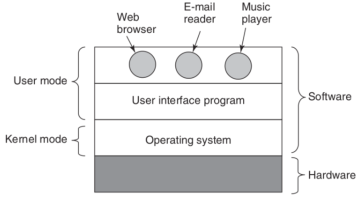
\includegraphics[width=0.85\textwidth]{FIG/1-1.pdf}
		\caption{操作系统所在的位置}\label{fig:fitin}
	\end{figure}

	同时,在许多系统中,一些用户态的程序协助操作系统完成特权功能。例如,经常有一些程序允许用户们修改密码,但是这个程序不是操作系统的一部分也不运行在内核态,但是它执行明显的敏感功能,并且必须以某种方式给予保护。
	在一些系统中,这个想法被执行到了极致,一些传统的被认为是操作系统一部分的程序运行在了用户态。在这些系统中,很难去划分一个界限,运行在内核态的明显是操作系统的一部分,然而运行在内核态之外的程序也有争议地被认为是操作系统的一部分,或者至少与其紧密相关。
	
	操作系统与应用程序的差异不仅仅在于他们所处的位置,特别地,操作系统更加大型,复杂和长期存在。像Linux和Windows这样的操作系统的核心代码都在500万行以上,要理解这个数量的含义,设想一下将500万行代码打印出来,每页50行,每卷1000页,将会需要100卷来打印出整个操作系统,需要一整个书柜来存放。你可以想象一下你获得了一个维护操作系统的工作,第一天你的老板把你带到存放代码的书柜面前,告诉你:学习这些代码吧。而这仅仅是运行在内核态的代码,当必要的共享库被包括进来的时候,Windows将会有将近7000万行代码,可以装满10-20个书柜。而这还不包括基础的应用程序(如窗口浏览器和媒体播放器等)。
	
	至于为什么操作系统的寿命较长,是因为它是非常难写的,一旦写了一个,所有者当然不愿意把它扔掉再重写一个。相反,操作系统会在长时间内进行演化。Windows 95/98/ME基本上是一个操作系统,Windows NT/2000/XP/Vista/Windows 7基本上是另一个操作系统。他们对于用户非常地相似,因为微软在努力使得Windows NT/2000/XP/Vista/Windows 7系统和Windows 98的系统非常相似。无论如何,微软要舍弃Windows 98是有非常好的理由的,我们将在第十一章中详细解释。除了Windows,我们在本书中用到的主要例子是UNIX以及它的变种和克隆版。UNIX当然也演化了很多年,如System V,Solaris和FreeBSD都是从该版本中演化出来的,尽管Linux像依照UNIX模式仿制而成,并且与UNIX高度兼容,但是其具有全新的代码基础。本书将采用来自UNIX的示例,并且在第十章中详细讨论Linux。
	
	在本章中,我们将简要触及操作系统的几个关键方面,包括它们是什么,它们的历史,有哪些分类,一些基本概念和它们的结构等。在后续的章节中,我们将详细介绍这些重要的内容。

\section{什么是操作系统}

	很难去给操作系统下一个明确的定义,操作系统是一个运行在内核态的软件,尽管这种说法并不完全符合事实。部分原因是操作系统扮演着两个完全不相关的功能,提供非应用程序编程人员一个清晰的资源集抽象而不是一堆混乱的硬件,并同时管理好这些硬件资源。取决于谁在谈论这个问题,你可能只会听到其中一个功能或另一个功能,让我们同时谈论这两个功能。
	
\subsection{操作系统作为一台扩展的机器}

	大多数计算机在机器语言级别的架构(指令级、内存组织、IO和总线结构)是原始的和难以编程的,特别是输入/输出。为了更细致地考察这一点,我们以在大多数计算机上使用的现代SATA硬盘位为例,曾有一本书描述早期版本的硬盘接口,一个程序员为了使用硬盘而应该了解的东西,超过了450页。自比2007年起,这个接口被修改了很多次,并且比那时候复杂了许多。很明显,没有任何一个理智的程序员想要在硬件层面和硬盘打交道,相反,他们使用一个叫做磁盘驱动的软件和硬盘打交道,这类软件提供了读写硬盘的接口,而不用去深入细节。操作系统包含了许多类似的控制IO设备的接口和驱动程序。但是即使是在这个层面,对于大多数应用程序而言还是太底层了。因为这个原因,所有的操作系统还提供另外一层使用磁盘的抽象:文件。使用这个抽象,程序可以创建、写和读文件,而不用去和底层硬件实际是如何工作的繁琐细节打交道了。
	抽象是管理这种复杂性的一种关键。良好的抽象可以将一个近乎不可能完成的任务转换为两个可以掌控的任务。第一步是定义和实现这些抽象,第二部是使用这些抽象来解决手头上的问题。一个几乎所有的计算机使用者都理解的抽象是文件,正如上文所提到的。它是一个有用的信息片段,像数字图片,保存的邮件消息,歌曲或者网页等。处理图片,邮件,歌曲和网页比处理SATA接口硬盘的细节要容易得多。操作系统的工作就是创建良好的抽象,并实现和管理它所创建的抽象对象。在本书中,我们将会讨论到许多关于抽象的内容,因为这是理解操作系统的关键。
	
	这点是如此地重要以至于它值得用不同的词语来重复描述。尽管出于对设计Macintosh机器的工程师的尊重,我们还是不得不说,硬件是丑陋的。真实的处理器、内存、磁盘和其他的设备是非常复杂的,对于那些必须使用它们来编写软件的人们而言,呈现出来的接口是困难、可怕、怪异和不一致的接口。有些时候这个是为了向后兼容更老一些的硬件,有的时候是为了节省成本。通常,硬件设计师们并没有意识到他们给软件的设计者们带来了多大的麻烦。操作系统的一个主要任务是隐藏硬件的细节,呈现给程序(和编程者)一个良好、清晰、简洁和一致的抽象。操作系统将丑陋转化为美丽,如图 \ref{fig:uglybeautiful} 所示。
	

	\begin{figure}[ht]\small
		\centering
		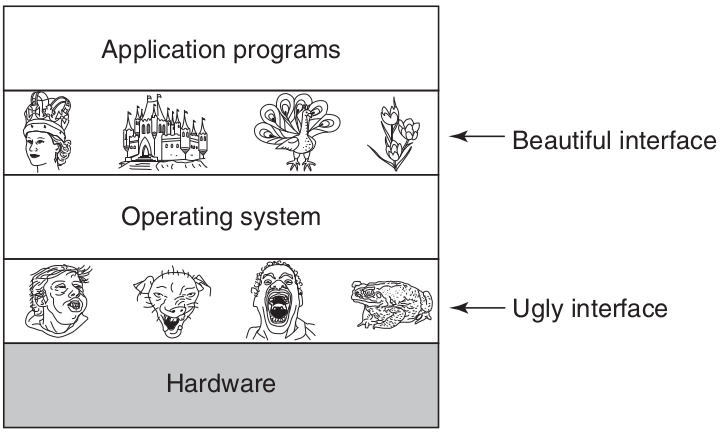
\includegraphics[width=0.75\textwidth]{FIG/1-2.png}
		\caption{操作系统将丑陋的硬件转化为美丽的抽象}\label{fig:uglybeautiful}
	\end{figure}

	值得注意的是,操作系统真正的消费者是应用程序(当然,通过应用程序的编程者),他们直接和操作系统及其抽象打交道。相比较而言,终端用户与应用接口所提供的抽象打交道,或者是命令行shell或者是图形用户界面。而用户接口的抽象可以和操作系统提供的抽象类似,但也不总是这样。为了更清晰地说明这一点,请读者考虑通常的Windows桌面和面向行的命令提示符。两者都运行在Windows操作系统上并且使用Windows提供的抽象,但是他们提供的是非常不同的用户接口。类似地,一个运行Gnome和KDE的Linux的用户和一个直接工作在X Window系统上的Linux用户看到的也是非常不一样的接口,但是两者的底层操作系统抽象是一致的。在本书中,我们将在细节层面讨论提供给应用程序的抽象,但是对于用户接口将讨论不多。尽管用户界面是一个重大且重要的主题,但是它只是与操作系统的外围相关。

\subsection{作为资源管理者的操作系统}

	把操作系统视为向应用程序提供抽象的概念是一种自顶向下的视角。按照另一种自底向上的视角,操作系统是用来管理一个复杂系统的各个部分。现代计算机包括处理器、内存、定时器、磁盘、鼠标、网络接口、打印机以及许多其他设备。在自底向上的视角,操作系统的工作是提供对需要处理器、内存和I/O设备等硬件资源的应用程序提供有序和可控的分配。现代操作系统允许在内存中同时运行多道程序,想象一下如果运行在同一台计算机上的三个程序同时想向打印机打印出它们的输出。第一个回合,我们将研究连续几代的计算机,看看它们的操作系统是什么样的,这种将操作系统的代际映射为计算机代际的做法是粗糙的,但是它确实提供了一种结构,否则就没有这种结构。接下来给出的进程主要是以时间顺序展开的,但是它又是一个颠簸的旅程。每一个发展阶段都不是等着上一个发展阶段完美地结束后才开始的,阶段与阶段之间有很多的交集,更不用说很多错误的开始和死胡同,请把这个作为一个向导,而不是一个定论。
	第一台真正的数字计算机是由英国数学家查尔斯·巴贝奇(1792–1871)设计的,尽管巴贝奇花费了他一生中大多数的时间与财富试图构建他的“分析机”,可是他从没有能够让它正常地工作,因为这个机器是纯机械式的,在当时他所在的年代,还不能制造出能够满足他所需的高精度的轮子、齿轮和轮齿。无需赘言,他的“分析机”也没有一个操作系统。
	作为一个有趣的历史旁白,巴贝奇意识到他的“分析机”可能需要软件,所以他就雇佣了一个叫阿达·洛芙莱斯的年轻女性作为程序员,她就是英国著名诗人拜伦勋爵的女儿,是世界上第一位程序员,编程语言Ada就是以她的名字命名的。
	
\section{操作系统历史}

\subsection{第一代(1945-55)真空管}

	在巴贝奇不成功的努力后,电子计算机的发展直到第二次世界大战之前取得了进步都很小,刺激了活动的爆发。John Atanasoff教授和他的研究生Clifford Berry在爱荷华州立大学建造了第一个功能式的电子计算机,它用了300个真空管。几乎与此同时,柏林的Konrad Zuse用机电继电器制造了Z3计算机。在1944年,一群科学家(包括阿兰图灵)在英格兰的伯克利公园制造和编写了Colossus机器,Howard Aiken在哈佛大学制造了Mark I,William Mauchley和他的研究生J. Presper Eckert在宾夕法尼亚大学制造了ENIAC。这些机器,一些用二极管,一些用真空管,一些是可编程的,但是都非常地原始,即使是进行最简单的计算也要耗用数秒钟的时间。
	在早年,同一小组的人们(通常是工程师们),设计、建造、编程、操作和维护每一台机器。所有的编程都是用绝对的机器语言完成的,更为糟糕的是,需要通过将上千根电缆插到插线板上连接成电路,以便控制机器的基本功能。没有程序设计语言(甚至连汇编语言也没有),操作系统更是从来就没有听说过。那时程序员一般的操作方式是,在墙上的机时表上预约一段时间,然后到机房中将他的插线板接到计算机里,接下来就是在接下来的几个小时里期盼计算机里的两万多个真空管不会被烧坏。那时,所有的问题都只是简单的数学和算术运算,如制作正弦、余弦、对数表或者是计算弹道轨迹等。
	在20世纪50年代,情形有了一定的改善,出现了穿孔卡片,这样就可以将程序写在卡片上,读入计算机而不再使用电路板,然后,其他的过程还是一样的。
	
\subsection{第二代(1955-65)晶体管和批处理系统}

	在上世纪50年代出现的晶体管的发明,极大地改变了这个状况。计算机已经变得很可靠,它们可以被制造、生产和出售给消费者,并且它们可以工作足够长的时间来完成一些有用的工作。就这样,第一次在设计者、制造者、操作者、编程者和维护者之间有了一个明确的分工。
	这些机器,现在叫做大型机,被锁在有专用空调的大机房里,有工作人员和专业操作者来运行他们。只有一些大型的公司,主要的政府机构和大学可以负担数百万美元的价格。为了运行一个任务,程序员需要首先将程序写在纸上(使用FORTRAN或者汇编语言),并把它做成有孔卡片,再将卡片盒带到输入室并把他交给操作人员,接下来就是边喝咖啡边等待输出结果的完成。
	
	当计算机完成了正在进行的任何的工作,操作者都要到打印机前撕下运算结果并把它带到输出室,以便程序员稍后收集、整理。然后,操作员将另一个卡片盒带到输入室并读入另一个任务。如果需要FORTAN的编译器,操作者需要将它从文件柜中取出并读入输入室中。大部分的机器时间在操作员在机器室中走来走去的时候被浪费掉了。

	因为设备具有这么高的成本,因此人们迅速地开始寻找降低所浪费时间的方法也就可以理解了。通常采用的解决方法是批处理系统(Batch System)。
	它背后的想法是将一堆工作收集起来放到输入室中,并用一个不太昂贵的机器例如IBM 1401将它读入磁带中,该机器非常擅长读取卡片,复制磁盘,打印输出结果,但是并不擅长数值计算。而真正擅长数值计算的机器,如IBM 7094,用来执行实际的运算。其情形如图 \ref{fig:batchsystem} 所示。
	
	\begin{figure}[ht]\small
		\centering
		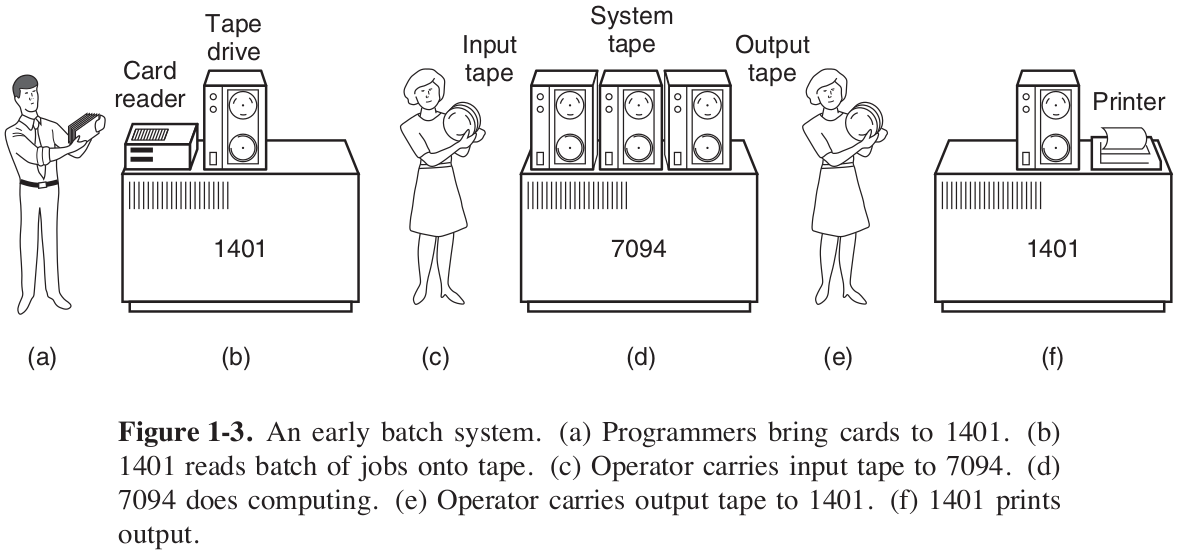
\includegraphics[width=0.75\textwidth]{FIG/1-3.png}
		\caption{一个早期的批处理系统}\label{fig:batchsystem}
	\end{figure}

	当一个完整的批处理过程结束的时候,操作员移除输入和输出的磁带,替换成下一批的输入磁带,并把上一批的输出磁带在一台1401的机器上离线打印出来(而不是连接主计算机)。
	
	一个典型的输入任务的结构如图 \ref{fig:FMS} 所示。它开始于一个\$JOB卡片,以分钟为单位设置好最大的运行时间,计费帐号以及程序员的名字。接着是一个\$FORTRAN卡片,告诉操作系统从系统磁带上加载FORTRAN的编译器,之后就是待编译的源程序,接着是一个\$LOAD卡片,直接地操作系统加载刚刚编译的目标程序。(编译程序通常被写在刮插磁带上并且需要被显式地加载)接下来是\$RUN卡片,告诉操作系统运行程序并使用随后的数据。最后,\$END卡片标志工作的结束。这个原始的控制卡片是现代shell和命令行解释器的先驱。
	
	\begin{figure}[ht]\small
		\centering
		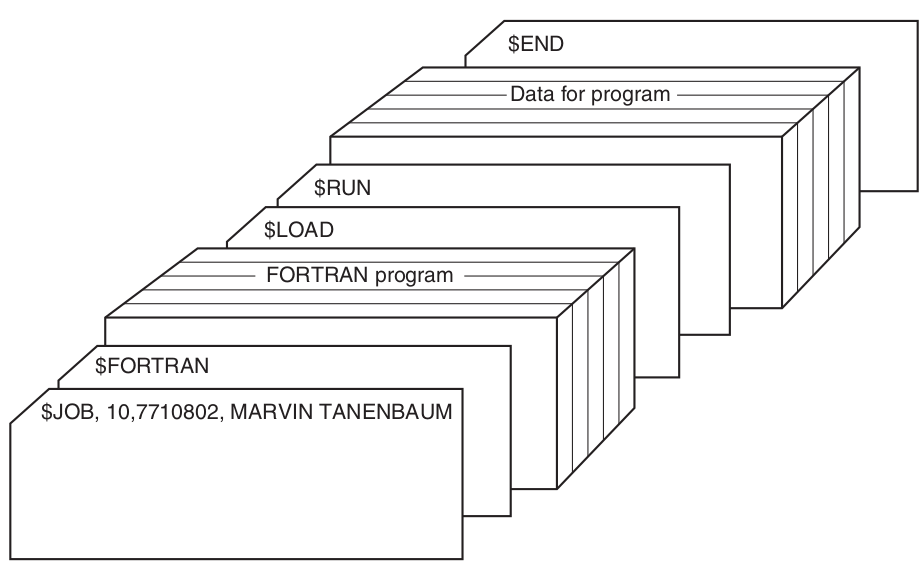
\includegraphics[width=0.75\textwidth]{FIG/1-4.png}
		\caption{一个典型的FMS作业结构}\label{fig:FMS}
	\end{figure}

	第二代大型计算机主要用于科学与工程计算,像在物理和工程中经常出现的解偏微分方程的程序,他们通常是使用FORTRAN和汇编语言编写的。典型的操作系统是FMS(Fortran Monitor System)和IBSYS,IBM的操作系统是7094。
	
\subsection{第三代(1965-1980)集成电路和多道程序设计}

	在上世纪60年代,大多数计算机生成厂商都有两条完全不同的,互不兼容的生产线。一种是是面向文字的,大规模的科学计算机,像7094,常用来在科学和工程领域进行工业级的数值计算。另一种是,面向字符的商用计算机,像1401机器,被银行和保险公司广泛地运用于磁带排序和打印上。
	
	发展和维护两个完全不一样的生产线对于生产厂商而言是一项昂贵的任务。此外,许多新的计算机消费者一开始仅仅需要一个小的机器,但是随着业务量的增长,他们需要一个更大的机器来运行他们的旧程序,但是需要运行地更快一些。
	
	IBM试图通过System/360系统来一举同时解决以上两个问题。360是一系列软件兼容的机器,从与1401机器相当的低端机器到与7094机器相当的高端机器。这些机器只是在性能和价格上(最大内存、处理器速度、允许接入的I/O设备的数量)的差别。因为他们拥有相同的架构和指令集,在一台机器上编写的程序可以在其他的任何机器上运行,至少理论上是。(但是,正像Yogi Berra说的这样,在理论上,理论和实际是一致的,但是在实际上,它们却不是。)因为360机器是被设计用来处理科学和商业计算,那么一个单系列的计算机可以满足所有客户的需求。在随后的几年里,IBM使用现代技术出产了360机器的后续机型,像370,4300,3080和3090。zSeries是这个系列的最新机型,不过它与早期的机型相比变化非常之大。
	
	IBM360机器是第一代采用小规模集成电路的主流机型,因此比采用分立晶体管的第二代的机器具有很高的性价比。360机器很快获得了成功,而且系列兼容机的想法很快被其他计算机制造厂商接受了。这些计算机的后代仍然在大型计算中心中使用,现在他们经常被用来维护大型的数据库系统(例如,航空订票系统)或者作为Web站点的服务器,这些服务器必须每秒处理上千次的请求。
	
	“单系列”想法的最大优点同时也是它的最大弱点。最初的意图是,所有的软件,包括操作系统OS/360原本都打算在所有的机器上运行。从小的能够替代1401机将卡片转换为磁带,到大的机器能够代替7094机器进行天气预报和其他繁重计算任务的计算任务。从只能带很少外部设备的机器到有很多外设的机器,从商业领域到科学领域。总之,它必须适用于所有的这些不同的用途。
	
	IBM无法写出能够同时满足这些相互矛盾的需求的软件,其结果是一个庞大而又复杂的操作系统,大概比FMS系统复杂2-3个数量级。它包括数千名程序员写的数百万行的汇编代码,同时包含数千个bug,这也导致IBM不断地发布新的版本来修正这些错误。每个新版本在修复就的bug的同时也引入了新的bug,因此bug的数量可能随和时间的变化而基本保持不变。
	
	作为OS/360的设计者之一的Fred Brooks,后来写了一本诙谐又尖锐的书籍来描述他对OS/360系统的经验。在这里不可能总结书中的内容,不过它的封面已经充分表达了它的观点,一群史前巨兽陷入了泥潭中不能自拔。Silberschatz书的封面也表达了类似的观点,操作系统像是恐龙一样。
	
	尽管OS/360有着巨大的规模和问题,OS/360和其他厂商开发的第三代操作系统实际满足了消费者大部分的需求。他们同时还使第二代操作系统中缺乏的几项关键技术得到了广泛的应用。其中一个重要的技术是多道程序设计(multi programming)。在7904机上,当当前的工作任务需要暂停来等待一个磁带或者I/O操作结束的时候,CPU仅仅是空闲等待I/O操作的完成。在CPU密集型的科学计算任务中,I/O操作是不频繁的,所以浪费的时间不是很明显。在商业数据处理的工作任务中,I/O等待的时间可能占用全部时间的80\%到90\%,所以必须采取某些措施来避免昂贵的CPU空闲这么久。
	
	所采用的方式是将内存分为几个分区,每一个分区中存放一个不同的作业,如图 所示。当一个作业在等待IO操作完成的时候,另一个作业可以继续使用CPU。如果有足够多的工作任务驻留在内存中,CPU可以保持接近100\%的使用时间。同时在内存中安全地保存数个工作任务,需要专门的硬件来保护每个工作被其他的工作所窥测和损害,360机器和其他的第三代系统都配备了这个意见。
	
	\begin{figure}[ht]\small
		\centering
		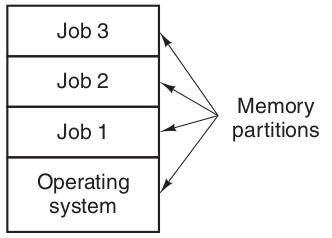
\includegraphics[width=0.65\textwidth]{FIG/1-5.png}
		\caption{一个有三个程序在内存中的多道程序系统}\label{fig:multiprogramming}
	\end{figure}

	第三代操作系统另一个主要的特征是具备了尽快将带到机房的磁带上的作业内容读取到磁盘上。因此,当一个运行中的作业停止的时候,操作系统可以从磁盘中加载一个新的作业到非空的内存区域中并运行它。这个技术叫做SPOOLing(外部设备联机并行操作),该技术也同时用于输出。因为有了SPOOLing技术,1401机器就不再需要了,而且也不需要将磁带搬来搬去了。
	
	尽管第三代操作系统非常适用于大型的科学计算和大部分商业数据的处理,它们基本还是批处理系统。许多编程者很怀念第一代机器的编程模式,那时他们可以单独占用机器好几个小时,从而可以调试自己的程序。在第三代操作系统中,从一个作业任务提交到获取输出结果通常需要好几个小时,因此一个分号的误用都有可能导致编译的失败,而可能浪费了程序员大半天的时间,程序员是非常不喜欢这种情况的。
	
	对快速响应时间的渴望对分时复用铺平了道路,一个多道程序的变化版,每一个用户都有一个联机终端。在一个分时系统中,如果有20个用户登录了系统,而其中有17个用户在思考,在交谈或者在喝咖啡,则CPU可以分配给三个需要服务的作业。因为人们在调试程序的时候经常使用较短的命令(编译一个5页的源文件)而不是较长的命令(对一个有100万件记录的文件进行排序)。计算机可以为一些用户提供快速的,交互的服务,或者在CPU空闲的时在后台同时处理的大型的批处理作业。第一代通用的分时操作系统CTSS,是在MIT基于一台修改的7904机器实现的。然而,分时复用系统没有得到及时的使用直到必要的保护硬件在第三代操作系统中出现。
	
	在CTSS系统成功之后,M.I.T.,贝尔实验室和通用电气(那时还是一个主要的计算机制造商),决定着手开发“计算机实用程序”,支持数百个同时分时用户的机器。他们的模型是电能系统,当你需要电能的时候,你只需要把用电设备插入墙上的插座即可,于是,在合理范围之内,所需要的电能随时可以提供。这个系统的设计者,被称作“MULTICS”系统,着眼于使用一个巨型的机器来为波士顿地区的每一个人提供计算能力。在当时看来,仅仅40年以后,就可以成百万台地卖掉比GE-645机器快1万倍的机器(价格远远低于1000美金),是纯粹的科幻,类似于现在的跨大西洋超音速海底列车的想法。
	
	MULTICS是一个混合的成功。它仅仅被设计在仅仅比基于Intel 386的PC机器强一点的机器上同时支持上百个用户,尽管它具有更高的I/O容量。可是这个想法并不用表面看上去这么荒唐,因为那个时候人们知道如何写小的、有效的程序,这个技能在后来逐渐消失了。MULTICS没有能普及到全世界是有很多原因的,其中一个重要的原因是它是用PL/I编程语言编写的,PL/I编译器的开发延迟了好几年,好不容易完成的编译器又很少能够正常地运行。当时,MULTICS有着很大的野心,就像19世纪查理斯巴贝奇的分析机器一样。
	
	简要地说,MULTICS向计算机文化中传播了许多原创的观念,但是要把它打造成一个严谨的产品和一个主要的商业成功则不那么容易。贝尔实验室放弃了这个计划,而通用电气也一起退出了个人电脑的业务。但是,MIT坚持了下来并让MULTICS最终得到运行。它最终被作为一个商业产品被收购了GE公司计算机业务的Honeywell公司出售,并且被超过80家的公司和大学安装使用了。尽管用户不多,但是MULTICS的用户是极度忠诚的。
	在试图让Honeywell公司更新硬件多年以后,通用汽车,福特,美国国家安全局在上世纪90年代末期才停止运行MULTICS,而这时距离MULTICS的发布已经过去了30多年。
	
	到20世纪末期,服务计算的概念已经被遗弃了,但是现在又以云计算的形式回归了,相对小的机器(包括智能手机、平板电脑)连接到遥远而又巨大的数据中心服务器在那里所有的计算都被完成,而本地计算机仅仅只是处理用户接口程序。这里的动机是多数人不愿意管理日益复杂的计算机系统,而更倾向于让运营、维护数据中心的专业团队去做这些事情。电子商务已经朝这个方向发展,许多公司都在多处理器服务器上运行邮件服务,简单的客户机连接到多处理器的服务器上,非常符合MULTICS的设计思想。
	
	尽管MULTICS没能取得商业上的成功,MULTICS对接下来的操作系统产生了及其重要的影响(特别是UNIX和它的衍生系统,如FreeBSD、Linux、iOS和Android系统)。详情请参考相关文献和书籍。还有一个活跃的网站,网址是www.multicians.org,上面有大量的关于该系统、设计者和用户的信息。
	
	第三代操作系统另一个重大的发展是小型计算机的崛起与快速发展,以1961年DEC的PDP-1机器为起点。PDP-1计算机只有4K个18位的内存,但是每台机器的售价是12万美元(仍不到7094机器的5\%),该机型非常地热销。对于一些特定的非数值型的计算任务,它和7904机器几乎一样快,并且催生了一个产业,并且很快有了其他一系列PDP机型(不像IBM家族,他们都是非兼容的),其顶峰为PDP-11。
	
	贝尔实验室的计算机科学家肯托马森,找到了一个无人在用的PDP-7小型计算机,开发了一个简化的、单用户版本的MULTICS,这个系统后来就发展成了UNIX系统,并且在学术界、政府机关和许多公司得到了广泛的使用。UNIX的历史已经在别处被多次讲述了,这段故事的一部分将在第10章中进行讲述。现在,因为源代码可以到处被得到,不同的组织会发展他们不同的版本,因而导致混乱。两个主要的版本被开发出来了,一个是AT\&T的System V系统,另一个是加州伯克利分校的FreeBSD系统,当然还有一些其他的小的变种。为了能够使编写的程序运行在任意的UNIX系统上,IEEE为UNIX开发了一套标准,该标准被称为POSIX标准,是现有大多数的UNIX支持的版本。POSIX定义了符合UNIX系统必须支持的最小系统调用接口。事实上,其他一些操作系统现在也支持POSIX接口。
	
	值得一提的是,在1987年,本书作者发布了一款UNIX的克隆版本,称为MINIX,用作教育目的。在功能上,MINIX非常类似与UNIX,包括POSIX的接口支持。从那以后,原来的版本已经演化为MINIX3了,它高度模块化,并且专注于非常高的可用性。它具有在不重启和不打扰其他运行程序的情况下,运行时检测和替换错误甚至是崩溃模块的能力,它致力于提高可用性和可靠性。有一本列出内部操作和在附录中列出源代码的书籍现在还有出售。MINIX 3系统是完全免费的,源代码可以在www.minix3.org上获得。
	
	对与MINIX系统自由产品的渴望,促使一位芬兰学生Linus Torvalds来撰写Linux。这个系统被直接受MINIX系统的启发,并且一开始就支持不同的MINIX的特征(例如,MINIX文件系统)。它被许多人在许多地方做了扩展,并且保持了许多与MINIX和UNIX类似的底层结构。对Linux的详细历史和开源运动感兴趣的读者们可能想读Glyn Moody的书,
	%在书中反复提到的是UNIX被应用到System V,MINIX,Linux和其他UNIX系统的克隆版本中去
	本书所包含的许多内容也同样适用于System V,MINIX,Linux以及UNIX的其他版本与克隆。

\subsection{第四代(1980-现在)个人计算机}

	随着大规模集成电路(LSI)的发展,在一平方厘米的硅片芯片上包含上千个晶体管,个人计算机的时代来临了。在架构方面,个人计算机(一开始称为微机)和PDP-11系列的小型计算机相比并没有很大的不同,但是在价格上却差别了很多。小型计算机的出现使得一个大学或公司的部分可以拥有自己的计算机,微处理器芯片的诞生则使得个人拥有自己的计算机称为了可能。
	1974年,Intel推出了8080CPU,第一款8位的通用CPU。它需要一个为8080设计的操作系统,一部分目的是为了对其进行测试。于是,Intel就安排了其顾问Gary Kildall来为8080CPU写操作系统。
	Kildall和他的朋友首先为新发型的Shugart Associates8英寸磁盘设计了一个控制器,并将软件连接到8080CPU,从而生产出第一台带有软盘的微型计算机。Kildall进而编写了一款基于磁盘的操作系统(CP/M (Control Program for Microcomputers))。因为Intel认为基于磁盘的个人计算机可能前途不大,当Kildall要求拥有对CP/M的所有权的时候,Intel答应了他的要求。Kildall进而创建了一个公司,Digital Research,来继续发展和销售CP/M。
	1977年,Digital Research公司重写了CP/M操作系统,使得它可以更好地运行在使用8080,Zilog Z80和其他CPU芯片的微型计算机上。并且基于CP/M编写了许多应用程序,使得CP/M系统主宰了微型计算机领域长达5年的时间。
	在20世纪80年代早期,IBM设计了IBM的PC并且寻找运行在其上面的软件。来自IBM的员工联系了Bill Gates来获得他的BASIC解释器的版权。他们还问他是否有运行在PC上的操作系统,Gates建议他们联系Digital Research公司,当时世界上操作系统的主流公司。作为有史以来最糟糕的商业决定,Kildall拒绝了和IBM的会面,而是让一名下属接待了他。更糟糕的是,他的律师甚至拒绝签署IBM关于对尚未公开的PC的保密协议。接下来,IBM公司只好回来找Gates,问他是否可以提供他们一个操作系统。
	
	当IBM回去的时候,Bill Gates想到一家当地计算机制造商,西雅图计算机产品公司,有一款合适的计算机系统,DOS(磁盘操作系统)。他与他们接洽并提出要购买这个操作系统,据说价格为75000美元,他们立即答应了。于是Gates提供给IBM一个DOS/BASIC的包,IBM接受了。IBM想要进行一些修改,所以Gate雇佣了写作DOS的人蒂姆·帕特森作为Gates的新公司微软的雇员也进行这项工作。被修改的系统被改称为微软DOS系统,并且很快地开始主导IBM的PC机市场。与Kildall试图将CP/M每次卖给一个用户相比(至少一开始是这样)相比,在这里一个关键的因素,后来也被证明是非常明智的决定的是Gates决定将他们的MS-DOS操作系统和计算机公司的的硬件绑定起来一起销售。在这所有的一切烟消云散之后,Kildall突然离开了人世,其原因至今仍没有被完全披露。
	
	IBM PC的继任者IBM PC/AT,在1983年随着Intel 80286CPU一起被开发出来。至此,MS-DOS的地位开始牢固确立,而CP/M只剩下了最后的支撑。MS-DOS后来被广泛使用于80386和80486CPU之上。
	尽管MS-DOS的初始版本非常地原始,后续的版本包含了很多高级的特征,包括许多从UNIX借鉴的特征。(微软对于UNIX是如此地娴熟,以至于在公司的早期还销售过一款叫做XENIX的微型计算机版本)
	
	早期的微型计算机的操作系统,CP/M,MS-DOS和其他的操作系统都是基于用户从键盘输入命令的方式。这种情况被斯坦福研究所的Doug Engelbart在上世纪60年代的研究所最终改变了。道格·恩格尔巴特发明了图形用户界面,有完整的窗口,图标,菜单和鼠标。这些想法被施乐PARC的研究人员采纳,并被融入到他们制造的机器中。
	
	一天,当史蒂夫乔布斯在他的车库中联合创建了苹果电脑公司,访问了PARC,看到了GUI,立即意识到了他的潜在价值,而Xerox管理层恰好没有意识到。这种战略失误的庞大比例,导致了名为《摸索未来》一书的出版。
	乔布斯随后着手设计了带有GUI的苹果计算机,这个工程导致了Lisa的诞生,但是由于价格过于昂贵导致了商业上的失败。乔布斯的第二次尝试,苹果的Macintosh电脑,取得了巨大的成功,不仅是因为它比Lisa便宜很多,而且还因为它是用户友好的。这就意味着它的用户不仅可以对计算机一无所知,而且可以完全没有任何学习的意图。在图片设计,专业数字图片和专业数字视频生产领域,Macintosh获得了广泛的应用,并且这些用户对Macintosh有着极大的热情。1999年,苹果公司采用了一种内核,它来自本是为替换BSD UNIX内核而开发的卡内基梅隆大学的Mach微核。因此,尽管有着完全不同的界面,但是Mac OS X是基于UNIX的操作系统。
	
	当微软决定构建MS-DOS的后继产品时,它受到了Macintosh电脑成功的强烈影响。它构建了一个基于GUI的桌面操作系统,最初是运行在MS-DOS之上的(它更像是一个shell界面而不是一个操作系统)。在接下来将近10年的时间里,从1985年到1995年,Windows都只是基于MS-DOS的一个桌面环境。然后,到了1995年,一个整合了许多操作系统特征的独立的Windows版本Windows95发布了。该系统仅仅将底层的MS-DOS系统用于启动和运行一些老的基于MS-DOS的程序。1998年,这个操作系统的一个稍作修改的版本Windows98发布了。但是,不管是Windows95还是Windows98,还都使用了大量的16位的Intel汇编语言。
	
	另一个Windows的操作系统,Windows NT(NT意味着New Technology),在一定程度上兼容Windows 95,但是其内部是完全重写的,它是一个完全的32位系统。Windows NT的主要设计者是David Cutler,他同时也是VAX/VMS系统的设计者,因此一些来自于VMS的系统也反映在了Window NT中。事实上,如此多的VMS的想法出现在Windows NT中,以至于VMS的所有者DEC公司,起诉了微软公司。法院对该案件的判决结果引出了一大笔需要用多位数字表达的金钱。微软公司期待NT的第一个版本将会打败MS-DOS和其他所有的Windows版本,因为Windows NT是一个巨大的超级系统,但是这个想法失败了。只有Windows NT 4.0踏上了成功之路,特别是在合作网络上。Windows NT 5.0在1999年初改名为Windows 2000。微软期待它成为Windows 98和Windows NT的替代者。
	
	不过这两个版本都不是很成功,微软稍后发布了Windows 98的另外一个版本Windows ME(千年版)。2001年,又发布了Window 2000的一个微升级版,我们称为Windows XP。这个版本运行的时间较长,并且替代了Windows的所有原始版本。
	
	版本的更替还在继续,在Windows 2000之后,微软将Windows家族分割成客户端和服务器端两条线。客户端基于XP和它的继承者,服务器端则包括Windows Server 2003和2008。第三条线,嵌入式系统也在随后出现。Windows的所有版本均已服务包的形式派生出各自的变种,这足以让系统的管理员以及操作系统书籍的作者感到温暖。
	
	2007年1月,微软终于发布了Windows XP的继承者,称为Vista。它有一个全新的界面,改善了安全性和许多新的和升级的用户程序。微软期望它可以完全地取代Windows XP,但是它并没有做到。相反,由于它对系统配置的较高要求,严格的版权条件和支持数据版权管理功能(一种使用户更难复制所保护资料的技术),使得它获得了大量的批评,负面报道不断。
	
	随着一款全新的且并不那么消耗资源的操作系统Windows 7的来临,许多人决定跳过Vista。Window 7并没有引入很多的新功能,但是它相对较小而且更为稳定。在不到3周的时间里,Windows 7就获得了比Vista在
	7个月内获得的更多的市场份额。2012年,Windows发布了Windows 7的继任者,Windows 8,一款针对触摸屏幕,拥有全新界面和感官的操作系统。微软希望这个操作系统会成为许多设备的主流操作系统:台式机,便携式电脑,笔记本电脑,手机,家庭影院电脑等主流的操作系统。然而,到目前为止,它的市场占有率的渗透远远慢于Windows 7。
	
	另一个在个人电脑操作系统市场上的有力竞争者是UNIX(以及它的不同变种)。UNIX在网络和企业服务器上很强,但是也经常出现在台式电脑,笔记本电脑,平板电脑和智能手机上。在基于X86架构的计算机上,Linux正在成为学生和越来越多的企业用户代替Windows的受欢迎的替代者。从一个侧面,贯穿本书我们都将使用术语X86来指代从1970年代开始8086相同指令集架构的现代处理器。
	
	有许多的AMD或者Intel公司生产的处理器,	在引擎盖下它们或许有一些不同,处理器是32位的或者64位的,单核或者多核的,流水线深的或者浅的,不一而足。不管怎么样的,对于编程者而言,它们看起来都是相似的,并且都可以运行35年前的代码。尽管这种不管是很重要的,我们将使用显式模型,并且使用X86-32或者X86-64来指示32位或者64位的变体。
	
	FreeBSD同样也是UNIX的一个流行变体,它来源于伯克利的BSD项目。所有的现代Macintosh的计算机都运行的是FreeBSD的修改版本(OS X)。在使用高性能RISC芯片的工作站上,UNIX也是一个标准配置。
	它的变体广泛应用于移动设备中,像运行iOS 7和Android的设备。许多UNIX用户,特别是有经验的编程人员,比起GUI更加喜欢使用命令行界面。所以,所有的UNIX系统支持一个在MIT生产的叫做X Windows的系统(也被称为X11系统)。这个系统处理基本的桌面管理,允许用户使用鼠标创建、删除、移动和改变窗口的大小。经常一个完整的GUI,像GNOM或者KDE,可以运行在X11之上,使得UNIX给人一种类似于Macintosh或者微软Windows系统的感觉,对于那些想要这样做的UNIX用户而言。
	
	开始发生在上世纪80年代中期的一个有趣的发展是,运行网络操作系统和分布式操作系统的个人计算机网络的增长。在一个网络操作系统中,用户可以感知到多台计算机的存在,并且允许从一台机器向另一台机器复制文件。每一台机器都运行自己的本地文件系统并且有自己的本地用户。
	
	网络操作系统和单处理器的操作系统有着基本的不同。它们显示的需要一个网络接口控制器和一些低级别的软件来运行它,同时,程序获得远程登录和远程文件访问权限,但是这些附属并不改变操作系统的一个本质结构。
	
	一个分布式操作系统,相比较而言,它对用户呈现的还是一个传统的单处理器系统,即使是它实际上是包含多个处理器。用户可能不会感知到他的程序在哪里运行,他的文件存放在哪里,这些都是由操作系统来自动和有效地处理的。
	
	真正的分布式操作系统不仅仅是对单处理器操作系统增添一点代码那么简单,因为真正的分布式系统和集中式系统在一些关键方面有着很大的不同。分布式系统,例如,同时允许应用程序运行在好几个处理器上,因而为了优化并行量需要更多复杂的处理器调度算法。
	
	网络中的通信延迟意味着这些算法必须运行不完全的、过时的甚至是错误的信息。而这在一个单处理器系统中却有根本的不同,因为单处理器系统中操作系统掌握着整个系统状态的全部信息。
	
\subsection{第五代(1990-现在)移动计算机}

	自从迪克特雷西侦探在1940年代的连环画中开始使用“双向无线电腕表”,人们就渴望拥有一台可以随身携带的通讯设备。第一台真正的移动电话出现在1946年,重达40公斤。如果你有一辆汽车的话,你就可以把它带到任何地方。第一台真正的手持移动电话出现在1970年代,重量约1公斤,是绝对的羽量级,它被亲切地称为“砖头”,很快每个人都想拥有一台。今天,移动电话的使用率几乎覆盖了全世界90\%的人口。我们不仅可以使用移动电话和腕表打电话,并且很快可以使用眼镜和其他可穿戴设备打电话了。更多的是,打电话本身并不是很有趣了,我们可以收发邮件、网上冲浪、和朋友聊天、玩游戏和在交通拥堵中导航,甚至不需要想它两遍(一切都是那么地习以为常)。
	
	尽管将电话和计算功能集成到一个像电话一样的设备的想法在1970年代就出现了,第一台真正的智能电话直到1990年代NOKIA发布N9000才出现,它在表现上包含了两个完全独立的设备:移动电话和个人数据助手。在1997年,爱立信公司为它的GS88"Penelope"手机创建了“智能手机”一词。
	
	现在,智能手机已经无处不在了,不同的操作系统之间的竞争也非常地激烈,而且前景比PC世界还要晦暗不明。在编写此书的时候,谷歌的Android系统占有统治地位的操作系统,苹果的iOS系统则稳居次席。但是这种情形并不一定总是这样,并且有可能在几年内又会发生变化。如果在智能手机领域有什么是清楚的话,那就是长期占用山峰的王者地位是不容易的。
	
	大部分的智能手机在头十年中运行的操作系统是Symbian OS。它是一些流行厂商如三星、爱立信、摩托罗拉,特别是诺基亚选择的操作系统。然而,其他的操作系统像RIM的Blackberry OS(在2002年的智能手机中发布)和苹果的iOS(在2007年通过iPhone发布)开始蚕食Symbian OS的市场份额。许多人推测,RIM会占据主流市场,而iOS将会是消费者设备的王者,Symbian的市场份额暴跌。在2011年,诺基亚抛弃了Symbian并且声称将把Windows作为其主要的平台。在一段时间里,苹果和RIM被视为宠儿,尽管它们还没有达到Symbian曾经的流行程度和统治地位。但是这些并没有持续很长时间,谷歌在2008年发布的基于Linux的操作系统Android很快就战胜了它的对手。
	
	对于手机的生产商,Android的优势是它是开源的并且在一个开放的许可证下可以免费获得。因此,他们可以很容易地对系统做一些小的修补并适用于自己的硬件。同时,他还有一个庞大的开发APP的开发者社区,这些APP大部分是用Java语言写的。尽管如此,过去几年的形势表明Android的这种统治地位可能也持续不了,Android的竞争者们急于抢占它的一部分市场份额。我们将在第10.8节详细地介绍Android。
	
\section{计算机硬件概览}

	操作系统是和运行在其上的硬件设备紧密相关的,它扩展了计算机的指令集并管理它的资源。为了让其工作,你必须知道很多关于硬件的知识,至少要知道硬件是如何暴露给编程人员的。因为这个原因,让我们简要地回顾一下现代个人计算机中的硬件。完了以后,我们可以开始探讨操作系统的细节以及它是如何工作的。
	
	概念上讲,一个简单的个人计算机可以被抽象为如图 \ref{fig:components} 所示的类似模型。CPU、内存和I/O设备都通过一个系统总线连接,并通过它与其他部件通信。现代的个人计算机有一个更加复杂的结构,拥有多条总线,我们将在后面陆续讨论到。对于现在的时间点来说,现在的模型是足够了的。在接下来的章节中,我们将简要地介绍这些组件并且探讨一些关乎操作系统设计者的硬件的属性。毋须多言,将有一个非常紧凑的总结,许多书都是关于计算机硬件和计算机组织的,两本最著名的是Tanenbaum和Austin(2012)以及Patterson和Hennessy(2013)编写的两本。
	
	\begin{figure}[ht]\small
		\centering
		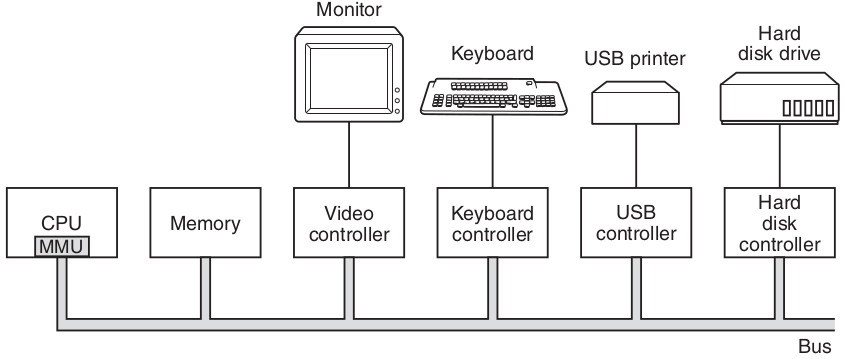
\includegraphics[width=0.65\textwidth]{FIG/1-6.png}
		\caption{一台个人计算机的主要组成部分}\label{fig:components}
	\end{figure}

\subsection{中央处理器}

	计算机的“大脑”是CPU。它从内存中获取指令并且执行它们。CPU的基本循环是从内存中获取第一个指令,解码这条指令来获取它的类型和操作数,执行它,接着再继续获取、解码和执行后续的指令,这个循环周而复始直到程序结束。通过这种方式,程序被执行。
	
	每一个CPU都有一个它可以执行的指令集,所以X86的处理器不能执行ARM的程序,ARM的处理器不能执行X86的程序。因为访问内存获取一条指令和数据比执行一条指令要花费很长的时间,所有的CPU都在内部保留一些寄存器来保存关键变量和中间结果。所以,指令集通常包含从内存中加载一个字段到寄存器的load指令,和将一个字段从寄存器存储到内存的store指令。其他的指令将来自寄存器、内存或者同时来自两者的两个操作数整合起来,像添加两个字段并且将结果存放在寄存器或者内存中。
	
	除了一些通用寄存器来存放变量和中间结果,大多数的计算机有几个对编程人员可见的专用寄存器,其中的一个是程序计数器,其中保存了下一条指令的内存地址。当那条指令被取出后,程序计数器的指针指向下一条指令。
	
	另外一个寄存器是栈指针,指向当前在内存中栈的顶部。栈包含每一个已经进入和尚未退出的程序中的一个页面,一个程序的栈页面保存这些没有存放到寄存器中的输入参数,局部变量和中间变量。
	
	另外一个寄存器是程序状态字(Program Status Word)。这个寄存器保存被比较指令设定的条件码位,CPU的优先权,模式(用户态或内核态),还有其他的各种控制位。用户程序可以读取程序状态字的所有位,但是只能写其中的某几个字段。PSW在系统调用和I/O中间发挥着重要的作用。
	
	操作系统必须对所有的寄存器实现完全的感知。当对CPU进行分时多路复用的时候,操作系统经常会停止目前正在运行的程序去启动或重启另一个程序。每次它运行一个程序,操作系统必须保存所有的寄存器状态,这样可以在后面重新启动被暂停的程序。
	
	为了改善性能,CPU的设计者们早就抛弃了同时取指、解码、执行一条指令的简单模型。许多现代的CPU具有同时执行一条或多条指令的功能。例如,一个CPU可以将取值、解码和执行单元分开,这样当它执行第n条指令的时候,它同时可以解码第n+1条指令和获取第n+2条指令。这样的一个组织称为流水线,在图 \ref{fig:pipeline} 中展示了一个流水线的三个阶段,更长的流水线也是常见的。在大多数流水线的设计中,当一条指令被取到流水线内的时候,它必须被执行,即使是它的前一条指令是一个条件分支。流水线给写编译器和写操作系统的人带来了巨大的麻烦,因为它将底层机器的复杂性暴露给了他们,而且他们还必须处理这些问题。

	\begin{figure}[ht]\small
		\centering
		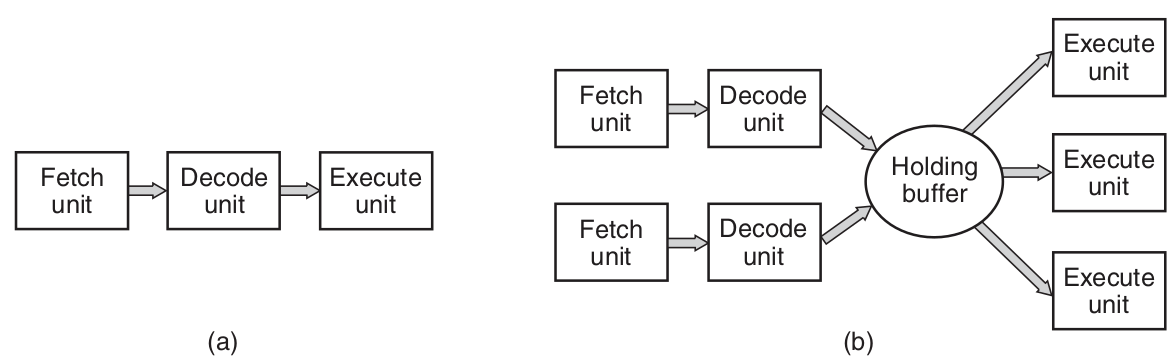
\includegraphics[width=0.75\textwidth]{FIG/1-7.png}
		\caption{一个三阶段的流水线和一个超标量CPU}\label{fig:pipeline}
	\end{figure}
	
	比一个流水线设计更为高级的是超标量CPU,如图 \ref{fig:pipeline}(b)所示。在这个设计中,会有多个执行单元,例如,一个是整数运算,一个是浮点数运算,另一个是布尔数字运算。两条或者更多的指令一次被取出,解码并被装入暂存缓冲区中直到他们被执行。当一个执行单元空闲的时候,它就会检查暂存缓冲区去看是否有它可以执行的指令,如果有的话,它将该指令从缓冲区中移除并执行它。这种设计的含义是程序指令经常是乱序执行的。在多数情况下,是由硬件来保证这种运算的结果和顺序执行指令时的结果相同,但是,仍然有部分令人烦恼的情形被强加给操作系统处理。
	
	大多数的CPU,除了一些用于嵌入式系统中的简单的CPU,大部分前面曾经提到过的两种模式:内核态和用户态。通常由PSW中的一位来控制。当运行在内核态时,CPU可以执行它的指令集中的每一条指令,并且可以访问硬件的每一个特征。在台式机和服务器机器上,操作系统通常运行在内核态,可以完全地访问硬件。在大多数的嵌入式系统中,只有一小段程序运行在内核态,操作系统剩余的部分运行在用户态。
	
	用户程序总是运行在用户态的,它只允许指令集中的一部分指令和硬件的部分特征被访问。通常情况下,所有涉及到I/O操作和内存保护的指令在用户态都是不被允许的。当然,设置PSW的控制位使进入内核态也是不被允许的。
	
	为了从操作系统获取到服务,用户程序必须通过系统调用(System Call)使得程序进入内核态并唤醒操作系统。TRAP指令完成从用户态到内核态的切换,同时启动操作系统。当这个工作完成的时候,控制权在系统调用之后的指令被返回给用户程序。我们将在本章的后续部分详细讨论系统调用的机理。暂时地,我们可以把它理解为一种可以使得操作系统从用户态进入和内核态的一种特殊程序。在排版方面,我们使用小写的Helvetica字体来在后续的文本中表示系统调用,例如:read。
	
	有必要强调的是,计算机使用陷阱而不是一条固定的指令来执行系统调用。大多数的陷阱是由硬件触发来对一些异常的情况发出警告,如除0和浮点数溢出等。在这些情况下,操作系统都得到完全的控制权并决定如何处理这些情况。有的时候,程序必须以一个错误状态终止,有的时候,则可以忽略错误(如对于下界溢出数可以设置为0)。最后,当程序预先声明要处理一些特殊情况时,可以将控制权交还给应用程序让其处理相关情况。
	
	\textbf{多线程和多核芯片}
	
	摩尔定律指出芯片上的晶体管数量每18个月会翻倍,这个定律并不是物理学上的诸如动量守恒之类的定律。而是Intel公司的联合创始人Gordon Moore的一个观察:在半导体公司的处理器工程师们可以以多快的速度缩减晶体管的数量。摩尔定律已经生效了将近30年,而且还有望至少再继续生效10年。到那个时候,每个晶体管的原子数目就会变得非常少,量子力学将会扮演主要的角色,这将限制晶体管数量的进一步缩小。
	
	大量地使用晶体管导致了一个问题,如果处理它们呢?我们看到了一个方法:带有多个功能单元的超标量体系结构。但是随着晶体管的增加,更多的晶体管也是有可能的。一个显然可以做的事情是在CPU芯片上放置更大的Cache,人们肯定会这么做,然后,原先获得的有用效果将最终消失。
	
	一个明显的步骤是不仅只复制功能单元,同时还复制一些控制逻辑。Intel奔腾4处理器中发布了这个属性,称为多线程或超线程,X86处理器以及一些其他的处理器使用了这个属性,如SPARC,Power5,Intel Xeon以及Intel Core系列的。近似地说,多线程是使得CPU保持两种不同的线程状态,并且能在纳秒级的时间内这两个状态之间进行切换。(线程是一种轻量级的进程,或者说是一个运行程序,我们将在第二章进行详细描述。)例如,如果一个进程需要从内存中读取一个字(需要花费多个时钟周期),则一个多线程的CPU就可以切换到另外一个进程,多线程并不提供真正的并行性。在某一个时刻只能有一个进程进行,只不过是线程切换的时间降到了纳秒级别。
	
	多线程对于操作系统而言是有意义的,因为每一个线程对于操作系统而言都像是一个独立的CPU。考虑一下实际有两个CPU的系统,每个系统有两个线程,操作系统将把它视为4个线程。
	
	除了多线程,许多的CPU芯片拥有四个、八个甚至更多的处理器和核心。图 \ref{fig:quadcores} 所示的多核芯片有效地搭载了四个子芯片,每一个子芯片都有自己独立的CPU(关于cahce后面再讨论)。有一些处理器,像Intel Xeon Phi和Tilera TilePro,已经可以在一个芯片上支持60多个核心了。为了充分利用这些多核芯片最终需要一个面向多处理器的操作系统。
	
	顺便说一句,就绝对数量而言,没有什么可以和现代GPU(图形处理器)相比,GPU是一种带有成千上万个微核的处理器,它们擅长处理大量的并发的简单计算,比如在图像应用中渲染多边形,它们不太擅长串行的工作,而且很难编程。尽管GPU对操作系统来说是有用的(加密或者处理网络拥塞),但是并不意味着操作系统本身可以运行在GPU上。
	
	\begin{figure}[ht]\small
		\centering
		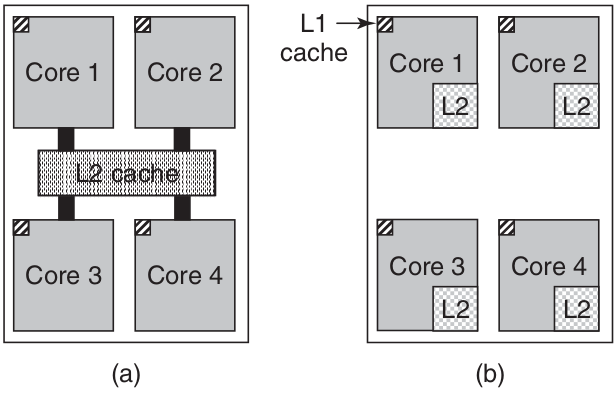
\includegraphics[width=0.75\textwidth]{FIG/1-8.png}
		\caption{一个四核的芯片共享一个L2缓存,一个四核的芯片每核带有独立的L2缓存}\label{fig:quadcores}
	\end{figure}
	
\subsection{内存}

	对于任何计算机而言第二重要的部件是内存。理想情况下,内存应该非常快(甚至比执行一条指令还快,这样CPU就不会被内存掣肘了),非常大而且非常便宜。现有的技术还不能满足以上这些目标,因此采取了另一个方法。内存系统是分层构造的,如图 \ref{fig:memoryhierarchy} 所示。上面的层次拥有比下面层次更快的速度,更小的容量和每字节更贵的价格,其差别往往是十亿数量级甚至更多。
	
	顶层是由在CPU内部的寄存器组成的,他们和CPU相同的材料组成,因此和CPU的速度一样地快。因而,CPU访问它们就不会有什么延迟,他们,它们的典型的存储容量配置是,对于32位的CPU是32 $\times$ 32位,对于64位的CPU是64 $\times$ 64位,都是小于1KB的。程序必须以软件的形式管理这些寄存器(决定把什么东西放进来)。接下来就是缓存内存,几乎是被硬件控制的。主内存被分割为缓存线,典型的是64字节,在缓存线0中的地址是0到63,在缓存线1中的地址是64到127,以此类推。最经常用到的缓存线会被存放到一个高速缓存区,其在CPU的内部或者离CPU非常近的地方。当程序需要读取一个内存字的时候,缓存硬件将会检查所需要的缓存线是否在缓存中。如果在,则称为缓存命中,请求直接在缓存区中得到满足,而不需要通过总线向主内存中发送内存请求。缓存命中通常会占用两个时钟周期,缓存没有命中则必须要到主存中请求数据,将会有巨大的时间代价。缓存的大小通常是受限制的,因为它的成本很高。有一些机器会有两层甚至三层的缓存,每一层都会比上一层空间更大,速度更慢。
	
	\begin{figure}[ht]\small
		\centering
		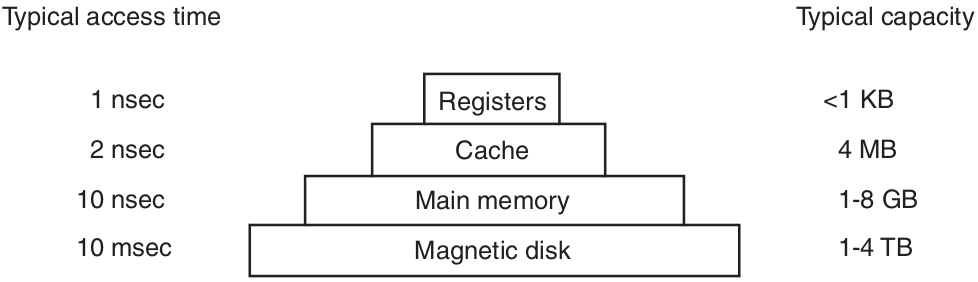
\includegraphics[width=0.75\textwidth]{FIG/1-9.png}
		\caption{一个典型的存储器层级,其中的数据均为粗略值}\label{fig:memoryhierarchy}
	\end{figure}

	缓存在计算机科学的许多领域中发挥着重要的作用,而并不仅仅是RAM的缓存。只要一种资源可以被分成许多的片,其中的一些比另外的一些使用地更加频繁,缓存都经常被用来改善性能。操作系统总是无时无刻不在使用缓存。例如,大多数的操作系统将经常使用的文件存放在主存中以避免经常重复从磁盘中读取这些文件。相似地,将类似「/home/ast/projects/minix3/src/kernel/clock.c」的长路经名转化为文件的磁盘地址可以被缓存下来,以避免重复地查找。最后,当一个网页的地址被转换为网络地址(IP地址),结果就可以被缓存起来供日后使用,还有很多其他应用实例。在任何缓存系统中,一个问题都是很快将会面临到的,包括:
	1. 什么时候向缓存中放入一个新的项目。 
	2. 新的项目放到哪一个缓存行中。
	3. 当需要一个空槽的时候,将哪一个项目移除缓存行。
	4. 将一个刚刚从缓存中移除的项目放到更大内存的什么位置。
	
	并不是每一个问题都会和每一个缓存情形相关。对于在CPU缓存中的主内存缓存行,通常在每次缓存未命中的时候都会进入一个新的缓存行。被使用的缓存线通常是通过被引用内存的高位来计算的。例如,对于64字节的4096缓存行以及32位地址,从第6位到第17位用来标识缓存行,第0位到第5位是在缓存行内部的。在这种情况下,要移除的缓存行可能和新的数据项一样,但是在其他系统中可能不是这样。
	最后,当一个缓存行被写到主内存中的时候(如果它在被缓存后有被修改过),被重写到内存中的地址则是由具体问题中的地址决定的。
	
	缓存是一个如此好的方法以至于现代的CPU都有两个缓存。第一层的缓存或者称为L1 Cache总是在CPU内部,总是解码指令到CPU的执行引擎中。大部分芯片对经常使用的数据字是有一个二级的L1 Cache,大部分的L1 Cache的大小是16KB。除此之外,还有一个经常使用的二级缓存,我们称为L2 Cache,在最近使用的内存字上通常有几MB的内容。L1缓存和L2缓存的区别之处是他们的时间。访问L1缓存是立即无延时的,访问L2级缓存则要延迟1-2个时钟周期。
	
	在一个多核的芯片中,设计者必须自己决定在那里放置缓存。在图 \ref{fig:quadcores} 中, 一个L2缓存是被所有的核心共享的。这个方法应用在Intel的多核芯片中。对比之下,图 \ref{fig:quadcores} 中显示的,每一个核心都有自己的L2缓存,AMD采用了这种方法。每一个策略都有自己的优点和缺点。例如,Intel共享L2级缓存需要一个更为复杂的缓存控制器,AMD采用的方法使得维持L2缓存的一致性更加地困难。
	
	在图 \ref{fig:memoryhierarchy} 中所示的层级结构中,接下来的一级是主存,这是内存系统的主力。主存通常又称为随机访问内存。过去又称为磁芯存储器,因为在20世纪50到60年代,使用小的可磁化的铁磁体来制造主存。它们已经绝迹了很多年,但是名字保留下来了。现在,内存的容量通常是几百MB到几个GB,而且还在快速地增长。所有的CPU的请求,如果缓存中不能得到满足的话,则将会访问内存。
	
	除了主内存外,许多电脑还有少量的非易失性随机访问内存。和RAM不一样的是,非易失性即使是在电源切断的情况下也不会丧失内容。ROM(只读存储器)是在工厂中加工好的,以后就不能再做更改,它速度快而且价格便宜。在一些计算机上,用于启动计算机的引导记载模块就存放在ROM中。而且,还有一些I/O卡采用ROM处理底层设备控制。
	
	EEPROM(Electrically Erasable PROM,电可擦除可编程ROM)和闪存(flash Memory)也是非易失性的,但是和ROM想反,它是可以重复擦写的。但是,擦写它们比写RAM要多花费几个数量级的时间,所以它们和ROM的使用方法一样,而其与众不同的特点是它们可以通过字段重写的方式纠正程序中的错误。
	
	闪存也便携式电子设备中也被广泛地应用。闪存被用于数码相机中的胶卷和便携式音乐播放器中的磁盘,这仅仅是闪存用途中的两项。闪存的速度介于磁盘和RAM之间,但是和磁盘不同的是,如果它被擦写多次的话,它会被写穿。
	
	另外一种类型的内存是CMOS,它是易失性的。许多计算机使用CMOS来保存现在的时间和日期。CMOS内存和增长时间的时钟电路是由一块小电池驱动的,因此,即使是计算机在没有上电运行的情况下,时间也可以被正确地被更新。CMOS内存同时还可以配置参数,如从哪一块磁盘中启动它们。CMOS被使用是因为它耗电很少,即使是使用出厂配置的电池也可以支持好几年的时间。但是,当电池被耗尽的时候,计算机开始呈现出阿兹海默氏症,开始遗忘持续数年的事情,如该从哪个磁盘启动等。
	
	\subsection{磁盘}
	
	在层次图中的下一个层级是磁盘。磁盘存储与内存存储相比,每一位要便宜两个数量级。同时,容量也要大两个数量级。唯一的问题是,它的随机访问数据的速度比内存要慢三个数量级。原因是,磁盘是一个机械设备,其结构如图 \ref{fig:disk} 所示。
	
	\begin{figure}[ht]\small
		\centering
		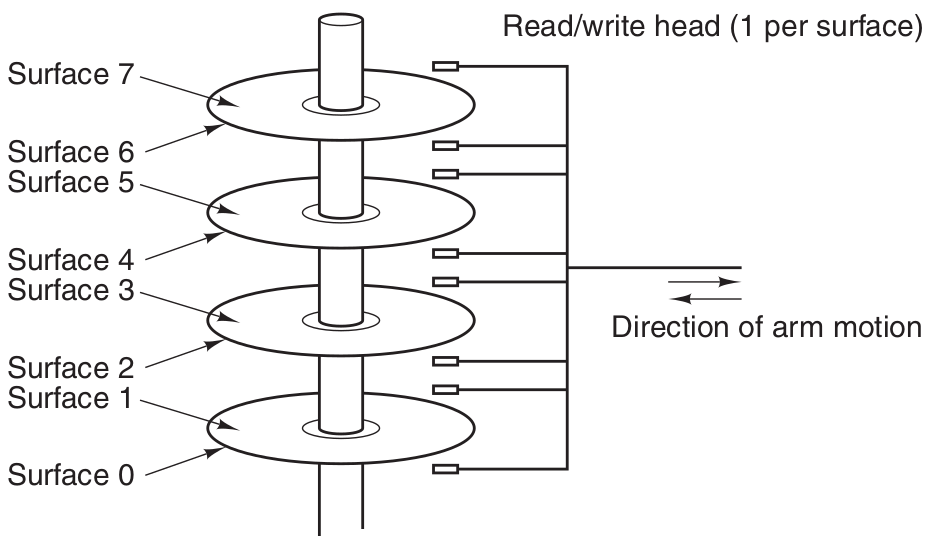
\includegraphics[width=0.75\textwidth]{FIG/1-10.png}
		\caption{一个磁盘驱动器的结构}\label{fig:disk}
	\end{figure}

	一个磁盘是由一个或多个每秒钟旋转5400转,7200转或者10800转的金属盘片组成的。一个机械臂从角落旋转到碟片上,类似于播放塑料唱片的老式33转/分留声机上的拾音器臂。
	
	信息被写道磁盘一系列的同心圆上,对于任意给定的磁盘位置,每一个磁头都可以读取一段环形区域,称为磁道(track)。把一个给定臂位置的所有磁道合并起来,组成一个柱面(cylinder)。
	
	每个磁道被分为若干个扇区,每一个扇区的典型大小是512字节。在现代磁盘中,外部的柱面比内部的柱面包含更多的扇区。将机械臂从一个柱面移动到另一个相邻的柱面大约需要1毫秒的时间,移动到一个随机的柱面大约需要5到10毫秒的时间,具体的时间取决于具体的磁盘驱动器。当扇区移动到相应的磁头下时,则开始读写,低速磁盘的速度为50MB/s,高速磁盘的速度为160MB/s。
	
	有时,你将会听到有人谈论实际上不是磁盘的磁盘,比如固态硬盘(SSD)。固态硬盘并没有可以移动的部分,也不包括像磁盘一样的盘片,它们是把数据存放到闪存中的。与磁盘的唯一相似之处是它们也存储了即使是关闭电源也仍然会保存的大量的数据。
	
	许多计算机支持一种称为虚拟内存(Virtual Memory)的机制,我们将在第三章中使用一定的篇幅介绍它。这种方法使得通过将它们放到磁盘上并且使用内存将最近经常使用到的部分缓存起来的方法来运行比主内存大的应用程序成为了可能。该方案需要动态地重新映射内存地址,将程序生成的地址转换为RAM中字所在的物理地址,这种映射是由CPU的一部分MMU部件完成的。
	
	缓存和MMU的出现会对性能产生很大的影响。在一个多道程序系统中,从一个程序切换到另一个程序称为上下文切换,这个过程需要刷新缓存中所有的被修改块和改变MMU中的映射寄存器。这两个操作的代价都很昂贵,程序员们非常努力地去避免他们。我们稍后将看到他们的战术的一些含义。
	
	\subsection{I/O设备}

	CPU和内存并不仅仅是操作系统所必须管理的资源。I/O设备也和操作系统有着很频繁的交互。就像图 \ref{fig:components} 所示的那样。I/O设备通常包含两个部分:控制器以及设备本身。控制器是一个或者一组物理性的控制设备的芯片。它从操作系统接收命令,例如,从设备中读取数据以及把它们取出。
	
	在大多数情况下,对于设备实际的控制是复杂的和充满细节的,因此控制器的工作是向操作系统提供一个更加简单的接口(事实上,仍然很复杂)。例如,一个磁盘控制器可能会收到一个从磁盘2读取11206扇区的命令。控制器必须将这个线性的扇区数转化为一个具体的柱面、扇区和磁头。这种转化可能会因为下面的情况而变得复杂:外部的柱面比内部的柱面拥有更多的扇区,一些坏的扇区必须被映射到其他的柱面上去。接着控制器必须决定悬臂放在哪一个柱面上,并且给它移入或者移出必须的柱面数的一个命令。它必须等到合适的扇区在磁头下旋转,然后开始读取和存储从驱动器上下来的位,去掉前导码并计算校验和。最后,它们必须将输入的比特组合成单词并把它们存放到内存中。为了完成这些工作,控制器经常包含一些小型的计算机来编程完成它们的工作。
	
	另外一部分是设备本身。设备拥有非常简单的接口,即是因为它们不能做太多的事情同时也是因为要将它们标准化。后者是十分重要的,这样所有的SATA磁盘控制器都可以处理SATA的磁盘。例如,SATA代表串行的ATA,而且ATA则是代表高级技术附件。如果你对AT代表什么表示好奇,它是IBM公司的"第二代个人电脑先进技术",它是1984年基于当时非常强大的6MHZ 80286处理器制造的。从中我们可以看出,计算机有着不断地用新的前缀和后缀来扩展首字母缩写词的习惯。我们还能看出,像“高级”这样的形容词应该谨慎使用,不然30年以后会显得非常可笑。
	
	SATA目前是许多计算机上的标准磁盘类型。因为真正的设备接口隐藏在控制器背后,所有的操作系统可见的是控制器的接口,这个接口可能和设备接口有着很大的区别。
	
	因为控制器的每一个类型都是不同的,每一个都需要不同的软件来进行控制。和控制器交互的软件,给控制器命令并且接收反应,称为一个设备控制器。每一个控制器厂商必须提供一个它所支持的操作系统的驱动。因此,一个扫描仪可能有OS X,Windows 7,Windows 8和Linux等不同的驱动。
	
	为了可以被使用,驱动程序必须被放到操作系统内部,这样他可以运行在内核态。驱动也可以运行在内核外部,像当前的类似Windows和Linux的操作系统也会提供一些类似的支持。绝大多数的驱动程序仍然运行在内核边界以下,只有很少的操作系统MINIX3,则在用户态运行所有的程序。运行在用户态的驱动程序必须被允许以一种受控的方式访问硬件,这种方式是不直接的。
	
	驱动程序被放入内核中可以有三种方式。第一种方式是将新的驱动程序重新连接到系统上并重启计算机,许多旧的UNIX系统是这样工作的。 第二种方法是在操作系统文件中输入一个条目,告诉它需要驱动程序,然后重新启动系统。在启动的时候,操作系统发现它所需要的驱动程序并加载它们,Windows就是通过这种方式工作的。第三种方法是让操作系统在运行时接受新的驱动程序,并且在不需要重新的情况下动态地安装他们。这种方式过去很少见,但是现在已经很普遍了。热插拔的设备,像USB和IEEE 1394设备,也同样需要动态地加载驱动。
	
	每一个控制器都有一小组与之交互的寄存器。例如,一个mini的磁盘控制器应该有识别磁盘地址、内存地址、扇区数、方向的寄存器。为了激活控制器,驱动程序从操作系统中获取一条命令,然后将其转换成适当的值写入设备寄存器。所有设备寄存器的集合构成了I/O端口空间,我们将在第5章中讨论这个主题。 

	在一些计算机中,设备寄存器被映射到操作系统的地址空间中去了,所以它们可以像普通的内存字一样进行读和写。在这些计算机上,无需特殊的I/O指令,用户程序可通过不将这些内存地址放在其可及范围内而远离硬件(通过使用基寄存器和限位寄存器)。 
	
	在其他的计算机上,设备寄存器都被放到一个特殊的I/O端口空间,每一个寄存器有一个端口地址。在这些机器中,提供在内核态使用的专门的IN和OUT指令,供设备驱动程序读写这些寄存器使用。
	前一种方法消除了对特殊指令的需要,但是很占用一些空间,后一种方法不使用地址空间,但是需要一些特殊的指令。两个系统目前都被广泛地使用着。
	
	实际输入和输出的方式有三种。在最简单的方式中,一个用户程序发起一个系统调用,内核将他们翻译成一个驱动设备程序的过程调用。然后,驱动程序启动I/O,并在一个紧密的循环中不断地轮询设备,看它是否完成了(通常有一些位表示设备仍在忙)。然后操作系统将控制权返回给调用者,这种方法被称为忙等待,它的缺点是占用了CPU的轮寻设备直到它完成。当I/O操作完成的时候,驱动程序将数据放置到它们需要的地方并返回。
	接着操作系统将控制权返回给调用者。这个方法被称为忙等待,其缺点是要占据CPU,CPU一直轮询设备直到对应的I/O操作完成。
	
	第二种方法是让驱动程序启动设备,并在完成的时候发出一个中断。设备驱动程序在这个时刻返回。操作系统紧接着阻止调用者并寻找其他工作来做。当控制器检测到传输结束时,它生成一个中断信号来完成。
	
	中断对于操作系统而言非常地重要,因此让我们多探讨一下它。图 给出了一个三步处理I/O的过程。在步骤1中,驱动程序告诉控制器
	接着控制器将启动该设备。当控制器已经结束要它传输的字节数的读或者写,在步骤2中,它使用某些总线线路向中断控制器芯片发送信号。
	如果中断控制器准备好接受中断(如果它正忙于处理一个高优先级的中断,则可能不是这样),则在步骤3中,它断言CPU芯片上的一个pin告诉它。
	在步骤4中,将设备的编号放在总线上,这样CPU可以读取它并知道哪个设备刚刚完成(许多设备可能同时运行)。 
	
	\begin{figure}[ht]\small
	 	\centering
	 	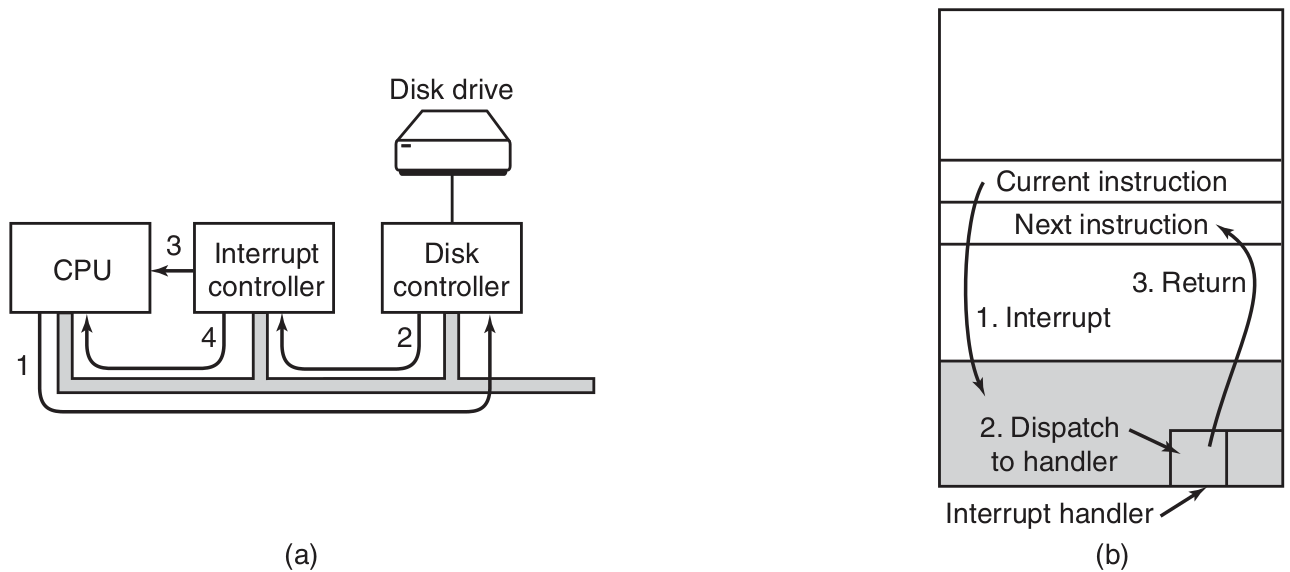
\includegraphics[width=0.75\textwidth]{FIG/1-11.png}
	 	\caption{a. 开启一个I/O设备并获得一个中断,b. 中断处理包括接受中断、运行中断处理程序并返回到用户程序。}\label{fig:interrupt}
	\end{figure}

	当CPU决定处理中断的时候,程序计数器和程序状态字通常会被压入到现在的堆栈中并且CPU被切换到内核模式。设备号可用作内存部分的索引来查找此设备的中断处理程序的地址。这部分的内存被称为中断向量。当中断处理程序(中断设备的部分处理程序)启动后,它移除堆栈程序计数器和PSW并保存他们,接着查询设备获得它的状态。当处理程序全部完成时,它返回到先前运行的用户程序,返回到尚未执行的第一条指令,步骤如图\ref{} 所示。
	
	第三种进行I/O的方法将采用特殊的硬件:一个DMA(Direct Memory Access)的芯片,它可以在不引起CPU干预的情况下控制内存和控制器之间的比特流。CPU安装这个DMA芯片,告诉它传输多少个字节,关联到的设备和内存地址,传输方向等,并且让他离开。当DMA芯片完成后,它将导致一个中断,按上述方法处理。DMA和I/O硬件将在第五章中详细讨论到。因此,CPU有一种方法可以禁用中断,然后在以后重新启用它们。当中断被禁用时,任何完成的设备都会继续断言它们的中断信号,但是直到中断被再次启用,CPU才被中断。如果多个设备在中断被禁用的时候完成,中断控制器决定先让哪一个设备先通过,经常是基于分配给每个设备的静态优先权决定的。拥有最高优先权的设备胜出并且第一个被服务到,其他的设备则必须等待。
	
	\subsection{总线}
	
	图 \ref{fig:components} 所示的组织结构在小型计算机以及最初的IBM PC上被使用了好多年。然而,随着处理器和内存变得越来越快,单个总线处理处理所有流量的能力达到了极限,必须要采取一些措施了。结果,额外的总线被增加了,同时对I/O设备和CPU对内存的速度都更快。这种演化的结果是,一个大型的X86系统看上去像现在图 \ref{fig:x86} 的样子。

	\begin{figure}[ht]\small
		\centering
		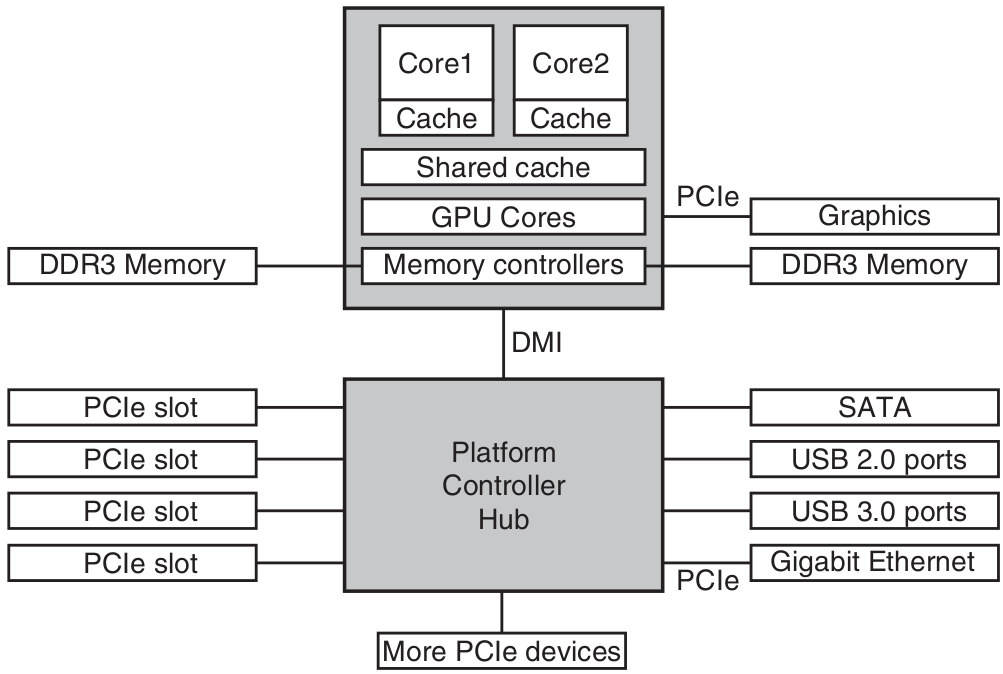
\includegraphics[width=0.75\textwidth]{FIG/1-12.png}
		\caption{一个大型X86系统的架构}\label{fig:x86}
	\end{figure}

	这个系统拥有很多的总线(像cache,memory,PCIe,PCI,USB,SATA和DMI),每一个都有不同的传输速率和功能。操作系统必须对它们进行配置和管理,主要的总线是PCIe(Peripheral Component Interconnect Express)总线。
	
	PCIe总线是Intel发明的作为更旧的PCI总线的一个后继者。PCI总线则是为了取代原来的ISA总线。每秒钟可以传输数十Gb的数据,PCIe比其前代的总线要快很多。它们在本质上也有很多的不同。直到发明PCIe总线的2004年,大多数的总线是并行和共享的,一个共享的总线架构意味着多个设备使用一条线来传输数据。因此,当多个设备都需要传输数据时,你需要一个仲裁者来决定谁可以使用总线。PCIe则恰好相反,它使用分离的,端到端的连接。例如,在通常的PCI总线上,一个32位的数字是通过32个并行的线传输的。和这个不同的是,PCIe使用串行总线架构并且通过一条被称为数据通路的链路传递集合了所有位的一条消息,这非常像网络包。这就简单了很多,因为你就不需要保证32位的数据在几乎相同的时间到达目的地。通过多个数据通路并行起来,并行性仍可以有效利用。例如,我们可以使用32个数据通路并行传输32条消息。随着像网卡和图形适配器等外部设备的速度快速地增加,PCIe的标准每3-5年就会更新一次。例如,PCIe 2.0规格的16个数据通道提供每秒64Gb/s的速度,升级到PCIe 3.0后速度会提升一倍,升级到PCIe 4.0后速度又会提升一倍。
	同时,我们还有很多符合老的PCI标准的旧设备。就像我们在图 \ref{fig:x86} 看到的一样,这些设备被连接到一个独立的集成处理器上。未来,当我们认为PCI不仅仅是“陈旧”,而且是“古老”的时候,很可能所有的设备将连接到另一个集成中心,这些中心再连接到主集成中心,从而形成一个总线树。
	在这种配置下,CPU通过一个快速的DDR3总线与内存进行交互,通过PCIe连接到外部图形设备,通过DMI(直接媒体接口)总线通过集线器连接到所有其他设备。集线器再连接到其他所有的设备,使用统一串行总线连接其他的USB设备,SATA总线连接磁盘和DVD设备,通过PCIe传输以太网络帧。我们已经提到了使用传统PCI总线的PCI设备。不仅如此,每一个核都有自己独享的一个缓存和一个更大的共享的缓存,每一个缓存都会引入一个总线。
	USB总线被发明用来将所有的低速的外部设备与计算机连接,像键盘和鼠标。然而,以5Gb/s运行的设备被认为很慢,这对于伴随第一代以8-Mbps的ISA总线为主要总线的IBM PC机长大的人们来说似乎并不自然。USB使用一个有4到11根线的连接器,有一些线是向USB设备提供电源的或者是地线。USB是一种集中式的总线,其根设备每1ms轮询一次所有的I/O设备看是否有信息收发。USB1.0可以处理总计12Mb/s的负载,USB2.0可以提速到480Mb/s,USB3.0则可以达到不小于5Gbps的速率。任何的USB设备都可以连接到计算机并且不需要重启计算机就可以立即工作,而不像之前的其他设备一样需要重启,这让一批沮丧的用户感到非常惊讶。
	SCIS(Small Computer System Interface)总线是专门为快速磁盘,扫描仪以及其他需要相当带宽的设备所设计的高性能总线。现在,我们经常可以在服务器和工作站中发现它们的身影,它们的速度可以达到640MB/s。
	要想在图 \ref{fig:x86} 所示的环境中工作,操作系统必须知道有哪些外部设备连接到了计算机并且对它们进行配置。这种需求导致了Intel和微软设计了一种即插即用的计算机系统,基于第一次在苹果的Macintosh上实现的一个类似概念。在即插即用之前,每一个外部设备有一个固定的中断请求级别和用于其I/O寄存器的固定地址。例如,键盘的中断请求级别是1,并使用0x60到0x64的I/O地址。软盘控制器的中断等级是6并使用0x3F0到0x3F7的地址,打印机的中断等级是7并使用0x378到0x37A的I/O地址,等等。
	到目前为止,一切正常。但是,当用户买了一块声卡和一块调制解调器,并且都使用中断4的时候,就会产生冲突而不能在一起工作,这个时候问题就产生了。解决方案是像每一个I/O卡上添加DIP开关和调节器,并且指导用户在系统中设定并选择一个不与其他设备冲突的中断等级和I/O设备地址。那些热衷于复杂PC硬件的十几岁的青少年可以不出差错地进行这项工作,而其他人则不能避免出错,这就导致了混乱。即插即用所做的工作是让系统自动地收集I/O设备的信息,集中地分配中断等级和I/O地址,并告诉每一块卡它的号码。这个工作和计算机启动的过程密切相关,所以接下来我们要探讨一下这个过程,这可不是一件轻松的工作。
	
	\subsection{启动电脑}
	
	简单地说,启动过程类似以下过程。每台计算机都有一个双亲板(在政治因素影响到计算机产业之前又叫母板),在双亲板上是一个叫做BIOS的系统程序。BIOS包含低级的I/O软件,包括读取键盘、写屏幕、做磁盘I/O以及一些其他事情的程序。现在,它被保存在一块非易失的Flash RAM中,但是可以在发现bug的时候通过操作系统来修改它。当计算机启动的时候,BIOS就开始工作了。它首先检查计算机中配备了多少内存,并检查像键盘以及一些其他的一些基本的I/O设备是否能够正常地反应。它通过扫描PCIe和PCI总线来开始检查所有与之连接的设备。如果当前的设备和上次系统启动时不一样,则被当作新设备配置。BIOS系统接着通过尝试存储在CMOS内存中的设备列表来决定启动设备。用户可以通过输入一个BIOS的配置程序而在重启之后立即改变这个列表。通常情况下会尝试从CD-ROM或者是USB设备进行启动,如果有一个是可行的话。如果失败了,BIOS则会从硬盘启动。启动设备的第一个扇区会被载入内存并被执行,这个扇区包含一段能够正常检测位于启动扇区尾部的分区表,来决定哪一个设备是活动的,接着从那个分区中读取二级启动加载器,这个加载器从活动分区中读取操作系统并启动它。接着,操作系统将需要BIOS来获取配置信息。对于每一个设备,它检查是否有设备驱动器。如果没有,它将让用户插入一个包含驱动器的CD-ROM(由设备制造厂商提供),或者从网上下载。当它具有所有的设备驱动时,操作系统将它们加载进内核。接着它将初始化表格,创建任何需要的后台线程,启动登录程序或者GUI界面。
	
	\section{操作系统大观园}
	
	操作系统已经存在了半个多世纪。在这段时间里,各种变种都被开发了出来,但是并不是所有的操作系统都很出名。在本节中,我们将讨论它们中的九个。在本书的后面,我们还将回顾一下几种不同的系统类型。
	
	\subsection{大型机操作系统}
	
	操作系统的高端是用于大型机的操作系统,它们是有房间大小的计算机仍然可以在大型公司的数据中心中看到。这些计算机不同于个人计算机在于它们的I/O容量。一个拥有1000块磁盘和数百万GB数据的大型机器是不罕见的,但是如果一台个人计算机拥有这个配置则会让朋友们很羡慕。大型机也在一些高端的网络服务器,大型电子商务网站的服务器,以及B2B业务中有一定的卷土重来。大型机的操作系统主要面向一次性处理很多工作的场景,他们多数都需要巨大的I/O能力。它们通常提供三种典型的服务:批处理、事务处理和分时。一个批处理系统是一个没有和现有用户交互的循环作业的过程。保险公司的索赔处理和连锁店的销售报告通常采用批处理的方式进行。事务处理系统处理大量的小的请求,例如,银行的支票处理和航班预订。每一个工作都很小,但是系统必须每秒种处理成百上千个这样的请求。分时系统允许多个远程系统同时在计算机上作业,如查询一个大型的数据库。这些功能是密切相关的,大型机操作系统通常完成所有这些功能。一个大机操作系统的例子是OS/390,是OS/360系统的后继版本。但是,大型机操作系统逐渐被诸如Linux的这类UNIX的变体所代替。
	
	\subsection{服务器操作系统}
	
	下一个层次是服务器操作系统。它们在服务器上运行,服务器可以是大型的个人机、工作站甚至是大型机。它们通过网络服务多个用户,并且允许用户共享硬件和软件资源。服务器可以提供打印服务,文件服务,Web服务等。Internet提供者运行很多的服务器机器来为消费者服务,网站使用服务器来存储它们的网页并处理来到的请求。典型的服务器操作系统有Solaris,FreeBSD,Linux和Windows Server 201x。
	
	\subsection{多处理器操作系统}
	
	目前获得大量联合计算能力的主要方式是将多个CPU连接到一个系统中。取决于他们是如何连接的以及共享了什么,这些系统被称为并行计算机,多计算机以及多处理器。他们需要专门的操作系统,但是经常是服务器操作系统的变种,配有通信、连接和一致性等专门功能。
	随着个人计算机多核芯片的出现,即使是传统的台式机或者笔记本都开始需要处理小规模的多处理器,而且核心数随着时间的增加而不断增加。幸运的是,由于先年的研究,已经具备了多处理器操作系统很多的知识,因此在多核系统中使用这些知识不是难事,难的是应用程序能够充分地利用这些计算能力。许多流行的操作系统,像Windows和Linux,都是运行在多核上的。
	
	\subsection{个人计算机操作系统}
	
	接下来的类别是个人计算机操作系统。现代的个人操作系统都支持多道程序,经常在启动的时候就有几十个程序开始运行了。它们的工作是对单个用户提供良好的支持。它们被广泛地应用于字节处理、电子表格、游戏及访问因特网等。通常的例子是Linux、FreeBSD、Windows 7、Windows 8和Apple的OS-X。个人计算机的操作系统是如此广为人知,因而不需要怎么介绍。事实上,许多人们甚至都感觉不到其他操作系统的存在。

	\subsection{手持计算机操作系统}
	
	接下来是越来越小的系统,我们来到平板电脑,智能手机以及一些其他的个人电脑。一个手持电脑,以往叫做PDA(个人数字助手),是一个可以在你手中操作的小型计算机。智能手机和平板电脑就是最好的例子。像我们已经看到的这样,现在的市场是由Google的Android和苹果的iOS占据了,但是它们也有很多的竞争者。大部分的这些设备有多核的CPU、GPS、照相机、其他的传感器、大量的内存以及复杂的操作系统。不仅如此,它们都有第三方的应用你可以摇一摇地下载它。	
	
	\subsection{嵌入式操作系统}
	
	嵌入式系统运行的计算机控制那些不被认为是计算机的设备,这些设备不接受用户安装的软件。典型的例子是微波炉、电视、汽车、DVD编码器、传统的电话以及MP3播放器。区别嵌入式系统和手持设备的一个主要特征是,嵌入式系统上不会运行不受信任的软件。你不能为你的微波炉安装一个新的应用程序,因为所有的程序都存放在ROM中。这就意味着操作系统不需要对应用程序进行保护,这就可以带来设计上的简化。系统像嵌入式的Linux、QNX和VxWorks都在这个领域比较流行。
	
	\subsection{传感器-节点操作系统}
	
	小型传感器网络被部署用于很多的目的。这些节点是小型的计算机,他们通过一个基站使用无线网络进行通信。传感器网络被用来保护建筑的外围,保卫国防边境线,检测森林火灾,测量温度和预报降水量,收集战场的敌人移动信息等。传感器是一种内置有无线电的电池驱动的小型计算机。它们的电能很有限,并且需要长时间在野外工作,而且通常是在环境恶劣的条件下。网络必须足够健壮以容忍单个节点的失败。随着电池的逐渐耗尽,这种节点会开始增加。每一个传感器电脑都是一个真实的计算机,有CPU、RAM、ROM以及一个或多个环境传感器。它运行一个小的,真实的操作系统,通常是一个事件驱动的,响应外部事件或者基于一个内部时钟进行周期性地测量。它的操作系统要求小和简单,因为节点的内存很小,电池寿命是一个重要的问题。同时,对于嵌入式系统,所有的程序都会被事先加载,用户不会突然启动他们从网上下载的应用程序,这样就使设计变得非常简单。TinyOS是一个广为人知的用于传感器的操作系统。
	
	\subsection{实时操作系统}
	
	另外一种类型的操作系统是实时操作系统,这些系统的特征是将时间作为关键参数。例如,在工业控制系统中,实时计算机需要收集生产过程相关的数据,并控制在工厂中的机器。通常,系统还必须满足严格的最终时限。例如,如果一辆汽车正在装配线上移动,必须在限定的时间内进行规定的操作。例如,如果焊接机器人焊接地过早或者过晚,都会损害汽车。如果动作需要在一个特定的时间(或者特定的时间段)出现,我们就需要硬实时系统(Hard Real-time System)。其中许多在工业过程控制、航空电子、军事等领域都有,以及类似的应用领域。这些系统必须提供绝对的保证,保证在某个特定的时间内会发生某个动作。
	
	一个软实时系统,是一个偶尔错过最后期限的系统,不可取,可接受,且不会造成任何永久性损坏。数字音频和多媒体系统属于这一个类别,智能手机属于软实时系统。有时候,操作系统仅仅是和应用程序相连接的一个库,各个部分必须紧密耦合而且部分与部分之间没有保护,这一类的实时系统是eCos。
	
	掌上,嵌入式系统以及实时系统的分类在一定程度上不少是互相重叠的。几乎所有的系统都具有软实时系统方面的特征。嵌入式系统和实时系统只运行系统设计者放入的软件,用户不能添加他们自己的软件,这样令保护变得更加简单。手持系统和嵌入式系统是专门为消费者设计的,而实时系统更多的是工业应用。不管如何,他们在一定程度上有相通之处。
	
	\subsection{智能卡操作系统}
	
	最小的操作系统运行在智能卡上,它们是一个信用卡大小的带CPU的芯片。它有非常严格的处理能耗和存储空间的限制。其中,有些是由插入读卡器的触点供电,但是非接触式的卡片是感应供电的,这大大限制了它们可以做的事。其中有些智能卡只能处理一个功能,像电子支付,而其他的卡片可以处理多个功能,它们有专用的操作系统。
	一些智能卡是面向Java的,这意味着在智能卡上的ROM有一个JVM的解释器。Java的小程序被下载到卡片上,并且被卡片上的JVM解释器执行。这些卡可以同时处理多个应用程序,从而导致多道程序并且需要去调度他们。当两个或更多的小程序运行的时候,资源的管理和保护也将会变成一个问题,这些问题都应该由卡片上的操作系统来处理。
	
	\section{操作系统概念}
	
	大多数的操作系统提供基本的概念和抽象,像进程、地址空间、文件等,它们是需要理解的核心内容。在接下来的章节中,我们将简单地考察这些基本概念中的一部分,在本书后面的章节,我们还将对其进行详细的讨论。为了解释这些概念,我们会时不时地使用例子,这些例子主要来源于UNIX。相似的例子同样会存在于其他的系统,我们后续会学习他们中间的一部分。
	
	\subsection{进程}
	
	所有的操作系统一个关键的概念是进程。进程就是一个在正执行的程序。伴随每一个进程的是它的地址空间,是一个从0到某一个最大值的内存位置的列表,可以供进程读和写。地址空间包含可执行的程序,程序的数据以及它的堆栈。同时,伴随每一个进程还有一组资源,通常包括寄存器(程序计数器和栈指针),打开文件的列表,突出的警报,相关进程的列表,以及运行程序所需要的其他信息。一个进程就是为了运行一个程序所包含的所有信息的容器。
	
	我们将在第二章中详细讨论进程的概念。不过,对进程建立起直观观念的一个最便利的方法是分析一个多道程序设计系统。用户可能打开了一个视频编辑程序并发出命令要把它转化为某种格式的一小时视频文件(这个过程可能要花费几个小时),接着他就去上网去了。于此同时,一个周期性的检查到来邮件的后台线程也开始运行了。这样,我们就至少有三个活动的线程:视频编辑器、网络浏览器以及邮件接收器。周期性地,操作系统决定停止运行一个进程而开始运行另外一个进程,那大概是因为在过去的一、两秒中,进程已经使用完了分配给它的时间片。
	
	当一个进程暂时被挂起,它在稍后必须将以停止前的状态被重启。这就意味着关于进程的所有信息在进程挂起的时候必须被显式地保存在某个地方。例如,进程可能会同时打开好几个用于读取的文件,同时还有每个文件当前位置的指针(字节数或者下一个将被读取的记录)。当一个进程被暂时挂起的时候,所有的这些指针必须被保存,这样在执行read系统调用重启进程的时候能够读取到正确的数据。在许多操作系统中,关于每一个进程的所有信息,除了它自己的地址空间的内容,都被保存到一个叫做进程表的操作系统表中,是一个结构的数组,每一个元素代表当前存在的一个进程。
	
	所以,一个挂起的进程包括它的地址空间,通常称为核心镜像(为了纪念以前用到的磁芯存储器),以及它的进程表项,包含了它的寄存器的内容,还有一些稍后重启进程时所必须的一些其他选项。
	
	与进程管理相关的关键的进程管理系统调用是那些创建和终止进程的系统调用。我们来考虑一个典型的例子,有一个叫做命令解释器或者shell的进程从终端读取命令。用户仅仅键入了一个要求编译一段程序的命令,shell必须创建一个运行编译器的新的进程。当这个进程完成编译的时候,它再执行一个系统调用终止自己。
	
	如果一个进程可以创建一个或多个其他进程(称为子进程),这些进程可以创建自己的子进程,我们很快就可以建立起类似图 \ref{fig:processtree} 所示的进程树。
	
	\begin{figure}[ht]\small
		\centering
		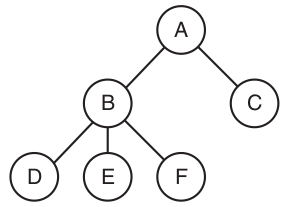
\includegraphics[width=0.75\textwidth]{FIG/1-13.png}
		\caption{一个进程树,进程A创建了两个子进程B和C,进程B创建了三个子进程,D,E和F。}\label{fig:processtree}
	\end{figure}

	相关的进程合作完成一个工作,经常需要和其他进程进行通信并同步它们的行为。这种通信称为进程间通信,我们将在第二章中详细描述。
	其他的进程系统调用可以要求更多的内存(释放没有被使用的内存),等待一个子进程结束,用一个程序覆盖另一个程序。
	
	有时,需要将信息传递给一个正在运行的进程,而该进程并不在等待此信息。例如,一个进程通过计算机网络向另一个远程进程发送消息,通过这种方式和另一台计算机上的进程进行通信。为了防止发送的消息或者它的回复丢失,发送者可能会要求它的操作系统在指定的若干秒后发一个通知,这样如果它还没有收到通知的话就可以重新传送。设置好这个定时器后,程序就可以做其他的工作了。
	
	当指定的若干秒过去后,操作系统向进程发送一个警报信号。这个信号将会导致进程挂起,不管这个进程现在正在做什么,保存它的寄存器在堆栈上,并且开始运行一个特定的信号处理程序。例如,重新传输可能丢失的进程。当信号处理结束的时候,正在运行的进程将会重新从信号之前的状态执行。信号是硬件中断的软件模拟,它可以因为各种原因而产生,除了定时器到期之外。许多陷阱是硬件检测出来的,如执行一个非法的指令或者使用一个非法的地址,也被转换成该信号并转交给这个进程。
	
	每一个使用系统的用户都会被系统管理者分配一个用户ID(UID)。每一个进程都有启动它的用户的UID,子进程和父进程拥有相同的UID。用户可以是组的成员,每个组都有一个组的ID(Group IDentification)。

	有一个UID,称为超级用户(UNIX)或者管理员(Windows),拥有特殊的权力,并且可以违背一些保护规则。在一些大型的安装中,仅仅只有系统管理者只要可以成为超级用户的密码,但是,许多的普通用户(特别是学生),投入了相当多的努力在寻找系统的漏洞上面,从而使他们不用管理员密码也可以称为超级用户。
	
	我们将在第二章讲述进程以及进程间通信。
	
	\subsection{地址空间}
	
	每一台计算机都有一些装载其正在运行程序的主内存。在一个非常简单的操作系统中,在某个时刻只有一个程序在内存中。为了运行第二个程序,第一个程序必须被移除,而把第二个程序放置到内存中。
	
	更多的复杂的操作系统允许多个程序同时驻留在内存中。为了防止他们互相干扰,需要一些保护机制。虽然这个机制是硬件形式的,但是它是被操作系统控制的。
	
	上述管理涉及对计算机主存的管理和保护。一个不同的,但是同等重要的与内存相关的主题是进程地址空间的管理。通常,每一个进程都有一套它可以使用的地址,通常是从0到一个最大值。在最简单的情形下,一个进程地址空间的最大值比主存的大小要小。这样,一个进程就可以填充它的地址空间并且有足够存放它的内存空间。
	
	然而,许多计算机的地址空间是32位或者64位的,地址空间大小分别是2$^{32}$到2$^{64}$字节。如果一个进程有比计算机主存更大的地址空间以及进程想全部使用这些内存的时候该怎么办呢?在早期的计算机中,这样的进程就没那么幸运了。现在,一个被称为虚拟内存的技术存在了,像前面提到的那样,操作系统将地址空间的一部分存放到内存中,一部分放到磁盘中,并且根据需要在它们之间来回穿梭。本质上说,操作系统建立了一个地址空间的抽象,作为进程可以引用的地址集。地址空间从机器的物理内存中被分离出来,并且不是比内存大就是比内存小。对地址空间和内存的管理形成操作系统一个重要的组成部分,我们将在第3章中谈论这个主题。
	
	\subsection{文件}
	
	被所有的操作系统支持的另一个重要的概念是文件系统。像前面提到的一样,操作系统的一个主要功能是隐藏磁盘和其他I/O设备的怪异性,并且呈现给编程者一个友好的、干净的、独立于设备的抽象模型。很明显,创建、删除、读取、写文件都需要系统调用。在读取一个文件之前,必须将它在磁盘上定位并打开,读取完毕之后则需要关闭它,这些都是系统调用做的事情。
	
	为了提供一个放置文件的场所,大多数的PC操作系统都有目录的概念用于将文件组合在一起。一个学生,例如,可能会有一个他正在上的课的目录,一个电子邮件的目录,一个存放万维网主页的目录。系统调用就需要创建和删除目录。系统调用还提供将一个文件放入目录和从一个目录中删除一个文件。目录项可以是文件也可以是其他的目录。这个模型也产生了层次结构-文件系统,像图 所示的那样。
	
	\begin{figure}[ht]\small
		\centering
		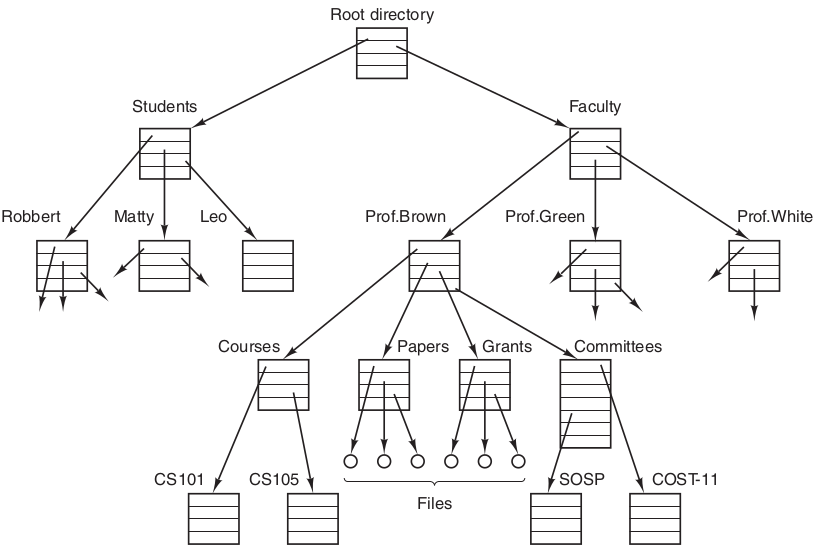
\includegraphics[width=0.75\textwidth]{FIG/1-14.png}
		\caption{一个文件系统的层次结构}\label{fig:fshierarcy}
	\end{figure}
	
	进程和文件层次都是按照树的结构来组织的,但是又有很大地不同。进程树通常不会很深(深过3层就不太正常了),然而文件层次却经常有4级,5级甚至更深。进程的层次通常是短暂存在的,通常最多只有几分钟,而目录层次却可以存在数年之久。进程和文件的所有者和保护机制也有很大不同。典型地,仅仅是一个父进程可以控制和访问一个子进程,但是对于文件和目录而言却需要允许所有者之外的其他很多用户来访问。
	
	目录层次结构中的每个文件都可以通过指定其路径来指定目录层次结构顶部的名称,根目录。这个绝对的路径名包含目录的列表,必须从根目录开始访问来获取这个文件,用斜线分离每一个组件。如图 \ref{fig:fshierarcy} 所示,文件CS101的路径是/Faculty/Prof.Brown/Courses/CS101。最前面的斜线说明该路径是绝对路径,是从根目录开始的绝对路径。顺便提及,由于历史原因,在Windows中,使用反斜线($\backslash$ )来代替正斜线作为分隔符。所以上述的文件路径在Windows下应该是$\backslash$Faculty$\backslash$ Prof.Brown$\backslash$ Courses$\backslash$ CS101。在本书中,我们通常采用UNIX的传统来代表路径。

	在每一个时刻,每一个进程都有一个工作目录,在其中查找不以斜杠开头的路径名。例如,图 \ref{fig:fshierarcy} 中,如果$\backslash$Faculty$\backslash$ Prof.Brown是当前的工作目录,使用路径Courses/CS101将生成与上面给出的绝对路径名相同的文件。进程可以通过发出指定新工作目录的系统调用来更改其工作目录。在一个文件被读和写之前,它必须先被打开,在此时将会检查权限。如果访问被允许了,系统返回一个称为文件描述符的小整数,用于后续操作。如果禁止访问,则返回错误代码。另外在UNIX中的一个重要的概念是挂载文件系统。大部分桌面台式机会有一个或者多个光驱可以插入CR-ROMs,DVDs和镭射光盘。它们也通常有USB接口,可以用来插入USB内存棒(实际上是固态硬盘),还有一些计算机有软盘和外置硬盘。为了提供一个处理这些可移动设备的优雅方法,UNIX允许这些在光盘上的文件系统可以被添加到主目录树上。考虑图 \ref{fig:mounting}(a) 的情形。
	
	\begin{figure}[ht]\small
		\centering
		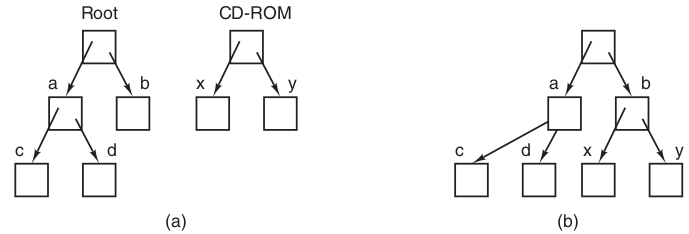
\includegraphics[width=0.75\textwidth]{FIG/1-15.png}
		\caption{(a)在挂载之前,CD-ROM上的文件是不可访问的,(b)挂载之后,它们称为文件目录的一部分。}\label{fig:mounting}
	\end{figure}

	在mount系统调用之前,在硬盘上的根文件系统,以及在CD-ROM上的二级文件系统,是独立的和不相关的。但是,无法使用CD-ROM上的文件系统,因为无法在其上指定路径名。UNIX不允许以设备名称或者设备号为开头作为前缀,这正是操作系统应该消除的对设备的依赖。
	相反,\texttt{mount}系统调用允许CD-ROM上的文件系统在程序想要的任何地方添加到根文件系统。图 \ref{fig:mounting}(b) 中,CD-ROM已经被挂载到目录b中,因此允许访问文件/b/x和/b/y。如果目录b
	包含有任何不能访问的文件而CD-ROM被挂载上了,/b指代的是CD-ROM的根目录。(无法访问这些文件并不像最初看起来那么严重:文件系统几乎总是安装在空目录上。)如果一个系统包括多个硬盘,它们也都可以被映射到一个目录树上。
	在UNIX中,另外一个重要的概念是特殊文件(Special File)。提供特殊文件是为了让I/O设备看起来像文件一样。这样,它们就可以使用同样的系统调用进行读和写,就像读和写文件一样。有两种特殊文件存在:	块特殊文件和字符特殊文件。块特殊文件用于对由随机寻址块(如磁盘)组成的设备进行建模。通过打开一个块特殊文件并且读取它们,例如,块4,程序可以直接访问到块特殊文件的块4,而不需要关心包含它的文件系统的结构。相似地,字符特殊文件用来模拟打印机、调制解调器、以及其他可以接收或输出字节流的设备。通常而言,特殊文件保存在/dev目录下。例如,/dev/lp可能是打印机(曾经称为行式打印机)。
	
	我们在概述中讨论的最后一个特征是同时和进程与文件相关:管道。管道是一种可以用来连接两个进程的伪文件,像图 \ref{fig:pipe} 所示的那样。如果进程A和B想通过管道进行对话,则它们必须事先安装好管道。当进程A想向进程B发送数据的时候,它把数据写在管道上,仿佛管道是一个输出文件。事实上,管道的实现也非常像是一个文件。进程B可以从管道中读取数据就好像读取一个文件一样。因此,UNIX中的进程间通信就非常类似于普通文件的读和写。更强大的是,进程发现它正在写入的输出文件不是一个真正的文件而是一个管道的唯一的方法是使用一个特殊的系统调用。文件系统非常重要,我们将在第四章、第十章和第十一章中详细讨论。

	\begin{figure}[ht]\small
		\centering
		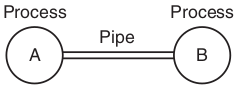
\includegraphics[width=0.75\textwidth]{FIG/1-16.png}
		\caption{连接两个进程的管道}\label{fig:pipe}
	\end{figure}

	\subsection{输入/输出}
	
	所有的计算机都有需要输入和产生输出的物理设备。毕竟,如果用户不能告诉它要做什么以及在做完之后不能得到工作的结果的话,那么计算机又有什么用呢。有许多种输入输出设备的存在,包括键盘、显示器、打印机等等。这取决于操作系统如何管理这些设备。所以,每一个操作系统都有管理其I/O设备的I/O子系统。一些I/O软件是设备独立的,即这些I/O软件部分可以同样应用于许多或者所有的I/O设备上。其他的部分,像设备驱动器,是专门为特定的I/O设备设计的。在第五章中,我们将讨论IO软件。
	
	\subsection{保护}
	
	计算机中包含大量的用户想要保护和设置为隐私的信息。这些信息包括邮件、商业计划、退税等诸多内容。管理系统的安全性完全取决于操作系统,例如,仅对授权用户访问。作为一个简单的例子,考虑一下安全是怎样工作的,请参考UNIX。UNIX中的通过分配给每一个文件9位的二进制保护码来保护文件。保护码包括三个三位的字段,一个用于所有者,一个用于与所有者同组的其他人员,另一个用于其他用户。每一个字段中有一个用于读访问,一个用于写访问,一个用于执行访问。这三个位就是所谓的rwx位。例如,保护码\texttt{rwxr-x--x}意味着所有者可以读、写和执行,同组内的其他成员可以读和执行该文件(但是不能写),而其他用户则只能执行该文件(不能读和写)。对于一个目录,x意味着检索权限,横线表示相应的权限是缺失的,没有的该当权限。除了文件保护之外,还有许多其他的安全问题。保护系统不受不合法的用户,包括人类和非人类(如病毒)的入侵,则是其中之一,我们将在第9章中讨论不同的安全问题。
	
	\subsection{Shell}
	
	操作系统就是一堆执行系统调用的代码。编辑器、编译器、汇编程序、连接程序、功能程序以及命令解释行等尽管它们非常重要,但是它们不是操作系统的一部分。冒着将事物弄得稍微有些复杂的危险,我们在本节中简单地介绍一下UNIX的命令行解释器,Shell。尽管它不是操作系统的一部分,但是它体现了操作系统许多重要的特性,并且很好地说明了系统调用的具体用法。Shell同时也是终端用户和操作系统之间的接口,除非用户正在使用图形用户界面。Shell有很多种,包括sh,csh,ksh和bash。所有的它们都支持下方描述的功能,这些功能可以追溯到早期的shell(即sh)。
	当任何一个用户登录的时候,一个shell程序就启动了。Shell程序有标准输入和标准输出的终端。它首先显示提示符(prompt),一个像美元符号的标识,告诉用户shell现在正在等待接收命令。如果这时候用户键入一个\texttt{Date}命令,shell就会创建一个子进程并且运行date程序。在子进程运行的时候,shell等待它终止。当子进程结束的时候,shell重新输出提示符,并且试图读取下一行。用户还可以将标准的输出重新定位到一个文件,例如:date > file。同样,标准的输入也可以重定向,像sort < file1 > file2,将会启动sort程序,从file1中读取输入,将结果输出到file2中。通过管道,可以将一个程序的输出变成另外一个程序的输入。像cat file1 file2 file3 | sort > /dev/lp,它将file1,file2,file3进行连接,并且将输出发送给sort程序,按照字符顺序对所有的行进行排序。sort程序的输出结果重新定位到文件/dev/lp上,通常是一个打印机。如果用户在命令后加上和号,shell不会等待它完成。相反,它只是立即给出提示符。结果,cat file1 file2 file3 | sort > /dev/lp \& 将会启动sort作为后台程序继续执行,这样将允许用户继续工作而sort程序也可以继续进行。shell还有一些其他很有趣的特征,我们在这里就不一一讨论了。有许多UNIX的书籍详细地讨论了shell(像Kernighan and Pike, 1984; Quigley, 2004; Robbins,2005)。今天,大部分的个人计算机都使用GUI,GUI实际上只是运行在操作系统之上的一个程序,像一个shell。在Linux系统中,这个事实更加明显,因为用户可以在两个GUI程序之间选择一个:Gnome和KDE,或者两个都不选(只是用一个X11的终端窗口)。在Windows中,也可以通过修改注册表中的一些值将标准的Windows桌面(Windows Explorer)改成另外的一个程序,尽管很少有人这么做。
	
	\subsection{胚胎重演律}
	
	在达尔文的《 物种起源 》一书出版以后,德国动物学家恩斯特·海克尔(Ernst Haeckel)说:“个体发育概括了系统发育。” 他这样说是意味着胚胎(个体发育)的发展重复着种群(系统发育)的演化。换句话说,在受孕以后,一个人类的胚胎在变成一个人体之前,经历了鱼,猪等发展阶段。现代的生物学家认为这是一种总体的简化,但是还是包含了内在的真相。在计算机工业也发生了类似的相似性,每一个新的物种(大型机、小型计算机、个人电脑、手持电脑、嵌入式电脑、智能卡)等,都经历了像他的祖先一样的发展历程,不管是硬件方面还是软件方面。我们经常忘记在计算机领域所发生的事情以及其他的很多领域都是技术驱动的。古罗马缺少汽车的原因并不是他们有多么地喜欢走路。而是因为他们不知道如何去建造汽车。个人计算机的存在不是因为数以百万计的人们压抑了数世纪之久的对计算机的渴望,而是因为现在可以很廉价地制造它们了。我们已经忘记了技术对我们的系统的视角影响有多大,这一点值得我们时不时地进行反思。特别的是,技术的改变常常会导致这个想法过时了,很快就消失了。然而,另外一个技术上的变化又可以让他重新复苏。这一点是绝对真实的,当需要对系统不同部分的相对性能而作出改变的时候。例如,当cpu比内存快很多的时候,缓存就变得非常重要来加速"较慢"的内存。如果有一天新的内存技术使得内存比CPU快很多的时候,缓存就会消失了。而如果一个新的CPU技术又比内存快很多的时候,缓存就会再次出现。在生物学中,灭绝是永恒的,但是在计算机技术而言,这些在短短数年之内就有可能发生。因为这种无常性,我们将在本书内经常提到一些"过时"的概念,一些对现有的技术不是最佳的想法。然而,技术上的变化又会使得一些"过时的概念"重新回到人们的视野。因为这个原因,弄清楚技术为什么会过时以及环境中的什么变化中会使得它再次复活就显得非常重要。
	为了更加明晰这一点,让我们考虑一个简单的例子。早期的计算机拥有无法改变的指令集,这些指令直接被硬件执行而且不能被更改。接着就产生了微程序(最初在IBM360机器上大规模引用的),一个底层的解释器用软件的形式解释"硬件指令"。硬连线执行就变得过时了,因为其不够灵活。接下来又发明了RISC计算机,这样微程序又过时了,因为硬件直接执行起来更快。现在我们看到解释执行正在以被发送到网络上在到达的时候解释执行的Java Applet小程序的形式复兴了。执行速度不总是最关键的因为网络延迟如此之大以至于他们往往占据着主导地位。因此,天平已经在直接执行和解释执行之间摇摆了好几个周期,而且未来还有可能会再次摆动。
	
	\textbf{大型内存}
	
	让我们来回顾一下硬件的发展历程以及它是如何影响软件的发展的。第一代的大型机拥有很有限的内存,一个完全配置的IBM 7090或者7094机器,从1959年末到1964年占据了山峰之上王者地位的机器,仅仅只有
	128KB的内存。它主要使用汇编语言编程,它的操作系统主要是使用汇编语言编写的以节约宝贵的内存资源。随着时间的推移,像FORTRAN和COBOL等语言的编译器变得足够好了,以至于汇编语言死亡了。但是,当第一代的商业小型机(PDP-1)发布的时候,它只有4096 18位字节的内存,汇编语言惊奇地杀了回来。最后,小型计算机需要更多的内存,高层次语言又变得流行起来了。
	
	当小型计算机在1980年代问世时,第一代计算机拥有4KB的内存,汇编语言又起死回生了。嵌入式计算机最初也使用和微型计算机一样的CPU芯片(8080s,Z80s和后来的8086s),最初也是在编译器中编程。现在,他们的继承者个人计算机,拥有更多的内存并且使用C,C++,Java和一些其他的高级编程语言进行编程。智能卡也正经历一个类似的发展过程,尽管超过了一定的规模,智能卡通常会有一个Java解释器并且解释性地执行Java程序,而不是让Java被编译成智能卡的机器语言。
	
	\textbf{受保护的硬件}
	
	早期的大型机器,像IBM的7090/7094机器一样,没有受保护的硬件,所以他们只是在一个时间运行一个程序。一个有bug的程序很可能会毁掉操作系统,并且使得整个机器崩溃。随着IBM360机器的问世,提供了保护硬件的原型。这些机器可以同时在内存中保存多个程序,并且让他们轮流执行(多道程序),单道程序就被认为是过时了。至少是到了第一个小型计算机出现时- 还没有保护硬件-这样多道程序就不可能的。尽管PDP-1和PDP-8没有保护硬件,而最终PDP-11有了,这个特征最终导致了多道程序和UNIX的诞生。当第一代微型计算机建造的时候,它们使用Intel的8080CPU芯片,其没有硬件保护,所以我们就回到了单程序编程,在内存中一次运行一个程序。直到Intel 80286硬件芯片,多道程序设计才成为了可能。直到今天,许多嵌入式系统还没有硬件保护而仅仅只是运行一个程序。
	现在我们来看一下操作系统。第一代大型机最初没有硬件保护也不支持多道程序编程,所以他们运行简单的操作系统,一次只能处理一个手动加载的程序。后来,他们获得了硬件和操作系统的支持,可以同时处理多个程序,这样他们一次就只可以手动加载一个程序。接着,他们就要求硬件和操作系统一次性支持和处理多个程序,然后是完全的分时能力。
	
	当小型机器第一次出现的时候,他们也没有保护的硬件,尽管那时多道程序设计在大型机领域已经很成熟了。逐渐地,他们要求硬件保护以及一次性运行两个或多个程序的能力。第一代的微型计算机的出现也可以在一次只运行一个程序,但是后来也要求运行多道程序。手持计算机和智能卡遵循同样的发展道路。
	
	在所有的情形下,软件的发展都是由技术决定的。第一代的微型计算机,大部分有4KB的内存和没有硬件保护。高级语言和多道程序对于这么小的一个系统而言就显得太多了。随着微型计算机演化为现代个人计算机,拥有了必要的硬件,接着开始要求软件开始处理一些高级的特征。这种发展很可能会持续数年。其他领域也可能有这种转世轮回,但在计算机行业似乎转得更快。
	
	\textbf{磁盘}
	
	早期的大型机器主要是基于磁带的。他们将会从磁带中读取程序,编译程序,运行程序并将结果写回到另一个磁带上。那时没有磁盘也没有文件系统的概念。这一切开始改变当IBM在1956年发布了它的第一款硬盘-RAMAC以后。它占据了差不多4平方米的地板面积可以存储500万7位的字符,这足够存储一张中等分辨率的图片。但是年度租金就高达35000美元,比存储占据同样空间数量的胶卷还要贵。不过磁盘的价格最终还是下降了,
	并开始出现了原始的文件系统。这些新开发的典型产品是CDC6600,它于1964年推出,多年来一直是世界上速度最快的计算机。用户可以创建所谓的“永久文件”,方法是给文件命名,并希望没有其他用户也认为“数据”是一个合适的文件名,这是一个单级目录。最终,大型机开发了复杂的分层文件系统,可能最终形成了MULTICS文件系统。
	随着小型计算机开始被使用,它们最终也有了硬盘。PDP-11在它1970年代被发布的时候,搭载的标准硬盘是RK05硬盘,大小为2.5MB,大约为IBM RAMAC硬盘的一半,不过其直径大约为40厘米,高度为
	5厘米。但是一开始也都是一个单层的目录。当微型机器开始出现的时候,CP/M是主流的操作系统,但是也只是在磁盘上支持一个目录。
	
	\textbf{虚拟内存}
	
	虚拟内存机制使得计算机可以运行比实际物理内存大的程序,通过在磁盘与内存之间快速地移动信息块的方式。它经历了一个类似的发展过程,一开始出现在大型机上,后来出现在小型机和微型机上。虚拟内存还允许程序在运行的时候使用动态链接库,而不是做内置编译。MULTICS是第一个这样做的系统。最终,这一思想传播开来并广泛应用于大部分的UNIX和Windows系统中。
	在这些发展中,我们会看到,在一个背景下被发明的东西,在另外一个背景下可能会过时(如汇编语言编程,单道编程,单层目录等),但是在下一个十年后可能又会重新出现。出于这个原因,在本书中,我们有时会看到一些想法和算法,这些想法和算法可能在今天的千兆个人电脑上过时,但很快就会在嵌入式计算机和智能卡上出现。 
	
	\section{系统调用}
	
	我们可以看到,操作系统有两个主要的功能,提供应用程序的抽象和管理计算机的资源。在大多数情况下,应用程序和操作系统之间的交互主要处理前者,例如,创建,写入,读取和删除文件。对于用户而言,资源管理部分主要是透明和自动完成的。所以,用户程序和操作系统之间的接口主要就是处理这些抽象。为了想真正了解操作系统干什么的,我们必须非常仔细地分析这个接口。接口中可用的系统调用因操作系统而异(尽管底层的概念是非常相似的)。我们需要在做出一个选择:(1) 模糊的一般性("操作系统有读取文件的系统调用")和(2) 一些特别的系统("UNIX有一个带有三个参数的系统调用:一个是识别文件,一个是告诉数据放到那里,另一个是读取多少个字节,另一个告诉读取多少个字节。") 我们选择采用后一种方法。尽管这个讨论特指POSIX(国际标准9945-1),以及UNIX,System V,BSD,Linux和MINIX3等,但是多数操作系统都有实现相同功能的系统调用,尽管他们实现的细节有很大不同。由于引发系统调用的机器是非常依赖于机器的,而且必须要以汇编代码表达,所以通过提供过程库使得C程序中可以实现系统调用,当然也包括其他的语言。
	
	记住下列事项是非常有益的。任何一个单CPU的计算机一次都只能执行一条指令。如果一个进程在用户态运行一个用户程序而需要一个系统服务,向从一个文件中读取数据,它需要执行一个trap指令向操作系统转移控制权。然后操作系统通过调查参数来判断进程想要什么。然后它执行系统调用并把控制权返回给系统调用后的指令。在某种程度上,执行系统调用就像是执行一个过程调用,区别仅仅在于系统调用进入内核而过程调用不进入内核。
	为了更加弄清楚系统调用的机制,我们来快速地看一下read系统调用。像前面提到的那样,它有三个参数:第一个参数指定文件,第二个参数指向缓冲区,第三个参数确定要读取的字节数。和所有的系统调用一样,它的调用由C程序通过调用一个同名的库过程read来完成。一个由C程序进行的调用,形式如下:count = read(fd, buffer, nbytes);
	系统调用(和库过程)以数字的形式返回实际读取的字节数,这个值通常和nbytes一样,但是也有可能会小一些,例如,在读取文件的时候遇到了文件的末尾。
	如果系统调用因为无效的参数或者磁盘错误不能被执行,counts的值将被设置为-1,错误号码将会放到一个全局变量中,errno。程序应该检查系统调用的结果,以了解是否出现了错误。
	系统调用是通过好几个步骤来执行的,为了将概念弄得更清楚一些,让我们看一下上面讲到的read系统调用。在准备调用实际启动系统调用的read库过程之前,调用程序首先将参数压栈,如图 \ref{fig:read11steps} 所示。
	
	\begin{figure}[ht]\small
		\centering
		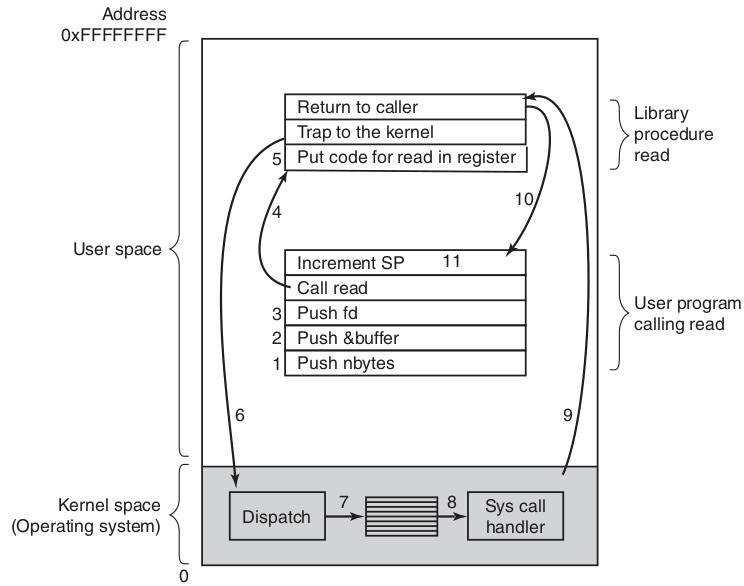
\includegraphics[width=0.75\textwidth]{FIG/1-17.png}
		\caption{调用read系统调用的11个步骤}\label{fig:read11steps}
	\end{figure}
	
	C和C++的编译器由于历史原因将参数以逆序的形式压栈(必须把第一个参数赋给printf(格式字符串),放在堆栈的顶部),第一个和第三个参数是通过值调用的,而第二个参数则是通过引用传递的,意味着缓冲区的地址(由\&指明)传递出去了,而不是缓冲区本身。接下来是真正地调用库过程(步骤4)。此指令是用于调用所有过程的正常过程调用指令。库过程,通常是用汇编语言写的,通常是将系统调用号放到操作系统所期望的一个地方,比如,寄存器中(步骤5)。接着它执行一个TRAP指令,从用户态切换到内核态,并从内核的一个固定地址开始执行(步骤6)。TRAP指令实际上和过程调用指令非常地相似,因为它后面的指令来源于一个遥远的位置,返回地址保存在堆栈上以备以后使用。不管如何,TRAP指令在两点上和过程调用指令不同。首先,是一个副作用,它将切换到内核态。而过程调用指令不改变这种模式。其次,不像给定过程所在的相对和绝对地址那样,TRAP指令不能跳到任意的地址上。根据机器的体系结构,或者跳转到单个固定地址上或者指令中有一个8位长的字段,它给定了内存中一张表格的索引,这张表格中含有跳转地址。
	跟随在TRAP指令后面的内核代码开始检查系统调用编号,并把它分配到正确的系统调用处理器,通常是通过一张由系统调用编号所引用的,指向系统调用处理器的指针表来完成(步骤7)。此时,系统调用处理器开始工作(步骤8)。一旦系统调用处理器完成了其工作,控制可以在TRAP指令之后的指令处返回给用户空间库过程(步骤9)。然后,此过程返回到中的用户程序通常的方法是调用return(步骤10)。为了完成这项工作,用户程序必须清理堆栈,就像它之后做的那样任何过程调用(步骤11)。假设堆栈是往下增长的,它通常情况下确实也是这样的,编译后的代码将堆栈指针的增量精确到足以删除在调用读取之前推送的参数。
	程序现在可以做它任何想做的事情了。
	在上面的9步中,我们提到:"控制可能会返回给用户空间库过程",这是有原因的。例如,如果它试图从键盘读入数据而没有得到任何的输入,那么调用者就必须被阻塞。在这种情况下,操作系统将会看一下有没有其他的进程可以运行。稍后,如果进程获取了想要的输入,进程将会获得操作系统的注意,并开始执行步骤9-11。
	在接下来的章节中,我们将会探讨经常会使用的POSIX系统调用,或者更具体地说,考察这些系统调用的库过程。POSIX大约有100个过程调用,图 列出了其中最重要的一些,为了方便我们把它们分为四类。接下来我们将简要地介绍一下每一个过程调用,以及它们是做什么的。在很大程度上,这些系统调用提供的服务决定了操作系统必须做什么事情,由于个人计算机上的资源管理功能是比较简单的(至少与多用户的大型机相比是这样)。所包含的服务包括创建和终止进程,创建,删除,读取,写入文件,目录管理以及完成输入/输出。值得指出的是,POSIX过程调用和系统调用并不是一对一的。POSIX标准指定了一个符合规范的系统必须提供的许多过程,但是它没有指定它们是系统调用、库调用还是其他什么。如果一个过程可以不执行系统调用而被执行(即可以不陷入内核态),它通常会因为性能原因在用户态执行。而然,大部分的POSIX过程将触发系统调用,经常是一个过程映射到一个系统调用上去。在一些情况下,特别是当几个过程之间只是很细小的区别时,通常是几个过程共同执行一个系统调用。
	
	\subsection{进程管理系统调用}
	
	\begin{figure}[ht]\small
		\centering
		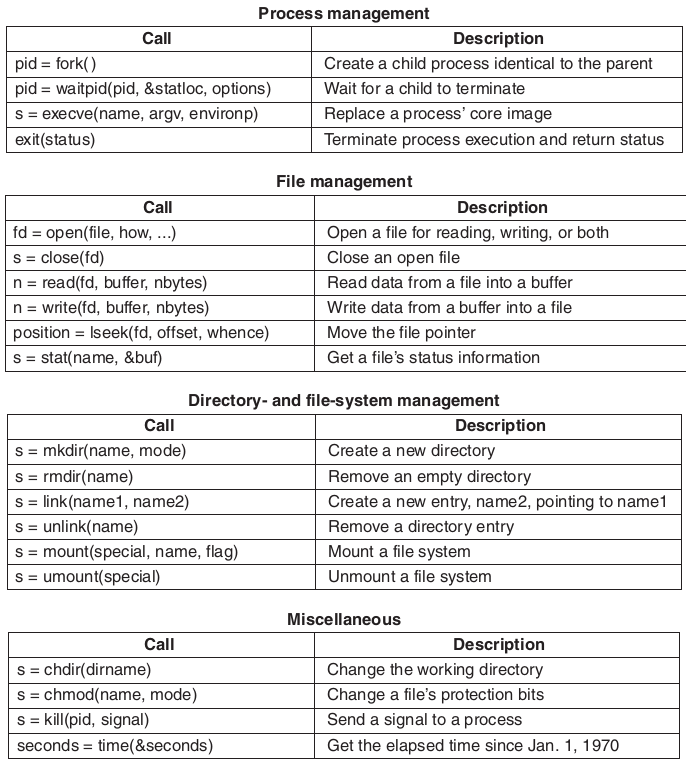
\includegraphics[width=0.75\textwidth]{FIG/1-18.png}
		\caption{一些主要的POSIX系统调用}\label{fig:systemcalls}
	\end{figure}
	
	在图 \ref{fig:systemcalls} 中的系统调用处理进程管理。Fork是一个可以开始讨论的好地方,Fork是POSIX中唯一一个创建新进程的方法。它创建了一个原始进程的精确副本,包括所有的文件描述符,寄存器等一切事物。在Fork之后,原始进程和副本进程各自走自己的路。所有的变量在fork的时候拥有相同的值,但是在父进程的数据完全被复制给子进程后,他们各自的后续变化将不再影响另一个(程序文本,是不可更改的,在父进程与子进程中共享)。Fork系统调用返回一个值,在子进程中是0,在父进程中是PID(Parent IDentifier),使用返回的PID,可以分别出哪一个是父进程,哪一个是子进程。
	在大多数情况下,在fork之后,子进程需要执行和父进程不同的代码,考虑一下shell的情况。它从终端处读取一条指令,派生子进程,等待子进程执行命令,当子进程结束的时候读取下一个指令。为了等待子进程结束,父进程执行一个\texttt{waitpid}系统调用,该系统调用只是等待子进程结束。\texttt{Waitpid}可以等待一个特殊的子进程,或者是任意一个旧的子进程,通过把第一个参数设置为-1。当\texttt{Waitpid}完成后,被第二个参数指向的地址,statloc,将被设置为子进程的退出状态(正常,异常退出和退出值)。通过第三个参数也可以有不同的选项,例如,如果没有子进程退出的话则立即返回。
	现在考虑shell是如何使用fork的,当一个命令被键入的时候,shell调用fork执行一个新的进程,这个子进程必须执行用户指令。通过使用execve系统调用来实现这一点,这将导致整个核心镜像被其第一个参数命名的文件所替换。(事实上,系统调用本身是exec,但是有几个库过程通过不同的参数和不同的名字。我们将在这里处理这些系统调用。) 图 \ref{fig:simpleshell} 是一个高度简化的shell阐述了fork,waitpid和execve是如何工作的。
	
	\begin{figure}[ht]\small
		\centering
		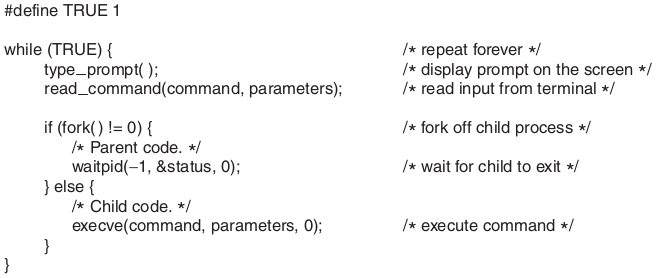
\includegraphics[width=0.75\textwidth]{FIG/1-19.png}
		\caption{一个精简的shell。贯穿全书,TRUE总是被定义为1。}\label{fig:simpleshell}
	\end{figure}

	在大多数的通常情况下,execve有三个参数:被执行文件的文件名,参数数组指针,环境数组指针,这些将会被很快地描述到。各种库过程,包括execl,execv,execle,execve,允许略掉参数或者以各种不同的方式指定。在本书中,我们在所有涉及的地方使用exec描述系统调用。让我们考虑一下向这样的命令:\texttt{cp file1 file2},是用来将file1复制到file2。在shell创建进程之后,该子进程定位和执行文件cp,并将源文件名和目标文件名传递给它。cp主程序(以及多数其他C程序的主程序)包括以下的声明:main(argc,argv,envp)。其中argc是命令行上的项目数的计数,包括程序名。对于上面的示例,argc是3。第二个参数argv是指向数组的指针。该数组的元素i是指向命令行上第i个字符串的指针。在我们的示例中,argv[0]将指向字符串“cp”,argv[1]将指向字符串“file1”,argv[2]将指向字符串“file2”。 
	%main函数的第三个参数,envp,是一个环境指针,是一个字符串数组,
	这些是程序可以获取环境变量的库过程,通常用于自定义用户希望如何执行某些任务(例如,要使用的默认打印机)。在图 \ref{fig:simpleshell} 中,没有环境变量被传递给子进程,因此exevc的第三个参数为0。
	如果exec显得过于复杂,不要绝望;它是最复杂的系统调用。其他的任何系统调用都更加简单。作为一个简单例子的系统调用,例如exit,完成执行时应该使用哪些进程。它有一个参数,退出状态(0到255),它通过\texttt{waitpid}系统调用中的\texttt{statloc}返回给父级。
	UNIX中的进程将内存分为三个段:文本段(程序代码),数据段(变量)和栈段。数据段向上增长,栈段向下增长,像图 \ref{fig:threesegments} 所示的那样。在它们之间是一段没有被使用的地址空间,堆栈会根据需要自动增长到间隙中,但数据段的扩展是通过使用系统调用brk显式完成的,brk指定数据段要结束的新地址。
	 
	\begin{figure}[ht]\small
		\centering
		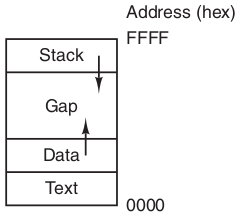
\includegraphics[width=0.75\textwidth]{FIG/1-20.png}
		\caption{一个进程有三个段:文本,数据和栈。}\label{fig:threesegments}
	\end{figure}
	
	数据段的扩展是显示通过一个系统调用brk实现的,它确定了数据段结束的新的地址。然而这个系统调用是没有被POSIX标准定义的,因为程序员被鼓励使用\texttt{malloc}库过程来动态分配内存,而\texttt{malloc}的底层实现则不是一个适合标准化的主题,因为几乎没有程序员直接使用它。我们甚至会注意到brk是不在系统调用之中的。
	
	\subsection{文件管理的系统调用}
	
	许多系统调用与文件系统相关。在本节中我们将看一下操作单个文件的系统调用。我们将在下一下涉及到目录或整个文件系统。为了读取和写一个文件,文件首先要先被打开。这个调用确定被打开的文件名,这个调用通过指定一个绝对的路径名和一个相对的工作目录名来指定要打开的文件名称,如代码O\_RDONLY,O\_WRONLY或者O\_RDWR意味着只读,只写和读写均可以。为了创建一个新的文件,会使用O\_CREAT参数。返回的文件描述符可以读或者写,接着,可以通过\texttt{close}系统调用关闭文件,它可以使文件描述符在后续的open中被再次使用。最经常被使用到的系统调用无疑是read和write。我们先看read系统调用,write系统调用拥有相同的参数。
	
	尽管大部分的程序是按照顺序访问文件的,但是一些应用程序需要能够随机访问文件的一部分。与每一个文件相关联的是一个指向文件当前位置的指针。当顺序地读或者写的时候,它经常会指向下一个被读/被写的字节。lseek系统调用改变了指针的位置,这样后续的read和write系统调用就可以在文件的任何位置停止。
	
	\texttt{lseek}有三个参数:第一个是文件描述符,第二个是一个文件位置,第三个是说明该文件位置是相对于文件起始位置,当前位置还是文件的末尾。lseek的返回值是改变指针后在文件中的绝对位置。
	
	对于每一个文件,UNIX跟踪文件模式(常规文件,特殊文件,目录等),大小,最后修改时间和一些其他的信息。程序可以通过调用stat系统调用看到这些信息。第一个参数指定了要被检查的文件,第二个参数指向一个指针,该指针指向存放这些信息的结构。对于一个打开的文件而言,fstat系统调用起到相同的作用。
	
	\subsection{目录管理的系统调用}
	
	在本节中,我们将讨论与目录和整个文件系统有关的系统调用,而不是上节中与某个文件有关的系统调用。mkdir和rmdir分别用于创建和删除目录,分别创建和移除空的目录。下一个调用是link,它的作用是允许一个文件以两个或多个名称出现,经常在不同的目录中。一个典型的应用是允许处在同一个编程小组的成员使用一个共同的文件,使得这个文件出现在他们每一个人的文件夹中,可能名字不同。共享一个文件并不等于给每一个成员一个私人副本,共享文件意味着任何成员所做的修改立即为其他成员所见--只有一个文件存在。而在复制了一个文件的多个副本之后,对其中一个副本所做的修改并不影响到其他的副本。
	
	为了看link是如何工作的,考虑一下图 \ref{fig:link} 所示的情形。这里有两个用户,ast和jim。每一个用户的目录下都有一些文件的。若ast现在执行一个包含系统调用的程序:link("/usr/jim/memo", "/usr/ast/note"),这个是将memo目录下的jim文件进入ast目录下的note文件。因此,/usr/jim/memo和/usr/ast/note指代的相同的文件。
	
	\begin{figure}[ht]\small
		\centering
		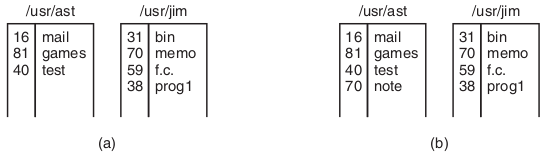
\includegraphics[width=0.75\textwidth]{FIG/1-21.png}
		\caption{a). 将/usr/jim/memo链接到ast目录之前的两个目录; b).链接后的两个目录}\label{fig:link}
	\end{figure}
	
	另外,用户目录是否保存在/usr、/user、/home或其他地方,这只是由本地系统管理员决定的。了解link是如何工作的可能会让它更清楚它的作用。UNIX中的每个文件都有一个唯一的编号,即标识它的i-节点号。这个i-节点号是i节点表的索引,每个文件一个,告诉谁拥有该文件,它的磁盘块在哪里等等。目录就是一个包含了对集合的文件。在第一个UNIX的版本中,每一个目录项是16字节,2字节的i节点号,14字节的文件名。现在,一个更复杂的结构用来支持更长的文件名。但是从概念上说,目录仍然是一个包含了若干文件的集合的文件。link所做的工作只是利用某个文件的i节点号,创建一个新的目录项。在图 \ref{fig:link}(b) 中,两个目录项拥有相同的i节点号,因为指向同一个文件。如果其中的任何一个稍后被删除了,如使用unlink系统调用,剩下的一个还在。如果两个都被移除了,UNIX看到尚且存在的文件没有目录项(i节点中的一个域记录着指向该文件的目录项),就会把该文件从磁盘中移去。
	就像我们之前提及的那样,\texttt{mount}允许将两个文件系统合并成一个文件系统。一个通常的情况是拥有根文件系统,包括经常使用命令的二进制(可执行)版本和其他一些经常使用的文件。在一个硬盘(子)分区上,用户文件在另一个(子)分区上。此外,然后用户可以插入一个包含要读取的文件的U盘。通过执行mount系统调用,USB文件系统可以被挂载到根文件系统上,像图  所示。
	一个典型的C语句完成mount操作的是:mount("/dev/sdb0", "/mnt", 0)。
	其中,第一个参数是USB设备的块特殊文件名,第二个参数是被挂载到目录树上的位置,第三个参数是告诉根文件系统被挂载的文件系统是读写的还是只读的。
	
	\begin{figure}[ht]\small
		\centering
		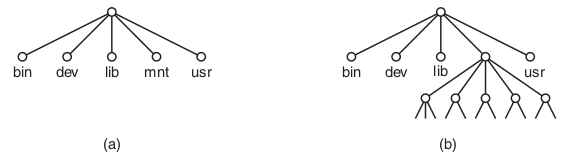
\includegraphics[width=0.75\textwidth]{FIG/1-22.png}
		\caption{a). 挂载前的目录树; b).挂载后的目录树}\label{fig:mount}
	\end{figure}

	在mount系统调用之后,一个在设备0上的文件可以使用从根目录或者工作目录的路径进行访问,而不用管文件在哪个设备上。事实上,还可以在这个树上挂载第二个,第三个,第四个设备。mount调用可以将可移动媒体集成到单个集成的文件层次结构,不必担心文件在哪个设备上。尽管这个例子讲述的是CD-ROM,但是可以用同样的方法挂载硬盘或硬盘的一部分,不管是外部的硬盘还是USB盘一样。当不再需要一个文件系统的时候,可以执行\texttt{umount}系统调用卸载文件系统。
	
	\subsection{各种系统调用}
	
	同样也存在着其他的系统调用。我们在这里只看他们其中的四个。\texttt{chdir}系统调用改变当前的工作目录,经过系统调用之后:
	chdir("/usr/ast/test"),将会打开一个xyz文件,/usr/ast/test/xyz,工作目录的概念消除了总是需要键入较长的路径名的需要。
	
	在UNIX中每一个文件都有一个用于保护的模式。这个模式包括针对所有者,组,其他拥有者的读-写-执行标志位。chmod系统调用可以改变文件的模式。例如,如果想改变某一个文件除了所有者之外为只读的,可以执行系统调用:chmod("file", 0644)。
	
	\texttt{kill}系统调用是用户和用户进程发送信号的方式。如果一个进程准备好了接收某一个信号,当它到达的时候,将会运行信号处理器。如果该进程没有准备好,那么信号的到来将会杀掉此进程(此调用名称的由来)。
	
	POSIX定义了一些处理时间的系统调用,如\texttt{time}系统调用,是以秒为单位返回当前时间,0对应着从1970年1月1日0时(从此时开始,没有结束)。在一台32位的计算机中,time的最大值是2$^{32}$-1秒(假设使用无符号整数)。这个值比136年稍大一些。因此在2106年,32位的UNIX系统就会变得发狂,与2000年对世界计算机造成严重破坏的Y2K问题是类似的。如果你现在有的是32位的UNIX系统,最好2106年之前换成64位的。
	
	\subsection{Windows Win32 API}
	
	到目前为止我们主要讨论UNIX,是时候讨论一下Windows了。Windows和UNIX的一个基本区别是他们的编程模型不同。UNIX系统包括各种处理事情的代码,使用系统调用执行特定的服务。与此相比,Windows通常是基于事件驱动的。主程序等待某一个事件的发生,然后调用一个程序去处理它。典型的事件有键盘被敲击,鼠标移动,鼠标按键按下或者插入了一个USB驱动。处理器将被调用来处理这些事件,更新屏幕和更新终端程序状态。所有的这些,都将会造成和UNIX不太一样的编程风格,但是由于本书的主题是讨论操作系统的功能和结构,我们将不会在关注这些编程模型的不同。
	
	当然,Windows也有系统调用。在UNIX中,系统调用和系统调用所使用的库过程几乎是一一对应的关系。换句话说,对于每一个系统调用,几乎都有一个触发它的库过程,像图 \ref{fig:read11steps} 所示中的那样。此外,POSIX有大约在100个过程调用。
	
	对于Windows,情况就大不相同了。首先,库调用和实际的系统调用是高度解偶的。微软定义了一组称为Win 32 API的过程调用供编程者使用获得操作系统的服务。这些接口支持所有的Windows 95以来的Windows操作系统版本。通过将API接口和实际的系统调用解偶,微软保持了在不改变现有程序的情况下随时改变系统调用的能力(甚至在每一个发行版本中进行改变)。
	
	是什么构成了Windows系统还是模糊不清的,因为最近版本的Windows有许多之前的版本所不包含的系统调用。在本节中,Win32意味着被所有版本的Windows支持的版本。Win32在Windows操作系统之间提供兼容性。
	
	Win 32 API的数量非常巨大,有上千个。此外,尽管它们中的许多触发系统调用,还是有大量的API完全是在用户态执行的。结果是在Windows无法分别哪个是系统调用(由内核执行),哪个是简单的用户空间库调用。事实上,在一个Windows版本中的系统调用可能在另一个版本中完全在用户态执行,反之亦然。当我们在本书中讨论Windows系统调用的时候,我们使用Win32过程,因为微软保障了随着时间的流逝,Win32过程将保持稳定。但是,值得记住的是并不是所有的它们都是系统调用(陷入到内核态)。
	
    Win 32 API有大量的系统调用,用来管理视窗,地理图标,文本,字体,滚动条,对话框,菜单以及GUI的其他特征。为了使得图形子系统运行在内核中(确实出现在某些版本的Windows中但不是所有的版本),需要系统调用,否则只有库调用。那么我们应该不应该在本书中讨论系统调用呢?由于它们和操作系统的功能并不相关,我们决定不讨论它们,尽管它们也是运行在内核中。对Win 32 API感兴趣的读者应该参考一些书籍中的相关内容(e.g., Hart, 1997; Rector and Newcomer, 1997; and Simon, 1997)。
    
   	尽管在这里介绍所有的Win32 API超出了问题的范围,所以我们只是将和UNIX系统调用功能大致相同的系统调用列出来在图 \ref{fig:win32APIs} 中。
   	
   	\begin{figure}[ht]\small
   		\centering
   		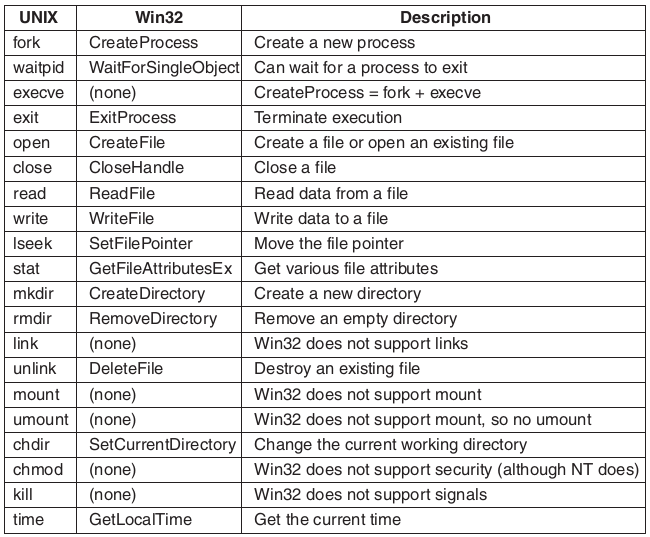
\includegraphics[width=0.75\textwidth]{FIG/1-23.png}
   		\caption{与UNIX大致对应的Win32 API} \label{fig:win32APIs}
   	\end{figure}
   
   现在让我们来简要看看图 \ref{fig:win32APIs} 中的内容。CreateProcess用于创建一个新的进程,它做的是UNIX中Fork加上execve的工作。它有许多的参数来指定新创建进程的性质。Windows不像UNIX那样具有进程层次结构,因为它不像UNIX一样具有父进程和子进程的概念。在一个进程创建后,创建者和被创建者是平等的。WaitForSingleObject被用来等待一个事件,可以等待许多可能的事件。如果有参数指定这个进程,调用者等待特定进程退出,通过调用ExitProcess完成。
   接下来操作文件的6个系统调用和UNIX的对应调用在功能上是类似的,尽管它们在参数和细节上有很多的不同。和UNIX中一样,文件可以被打开,关闭,读和写。SetFilePointer和GetFileAttributesEx调用用于设置文件位置和获取文件属性。
   Windows中有目录,它们使用创建目录CreateDirectory和删除目录RemoveDirectory API系统调用。也有对当前目录的标记,通过SetCurrentDirectory系统调用实现。使用GetLocalTime来获取当前的时间。
   
   Win32的接口不包括文件链接,挂载文件系统,安全,信号,所以对应与UNIX的这些调用就不存在了。当然,Win32也有大量的UNIX中没有的调用,特别是管理GUI的系统调用。Windows Vista有了一个精心设计的安全系统同时支持文件链接。Windows 7和8增加了更多的特征和系统调用。
   也许有必要对Win32做一下最后的说明,Win32并不是一个完全统一和一致的接口,最主要的原因是现有的32位Windows系统需要向后兼容16位的Windows 3.x系统。
   
   \section{操作系统结构}
   
   我们已经看到了操作系统从外面看是一种什么样的结构,现在是时候从里面看一下它的结构了。为了对各种可能的方式有所了解,我们将考察已经尝试过的6种不同的结构设计,这样并没有涵盖各种结构方式,但是至少给出了在实践中已经试验过的一些设计思想。我们将讨论的6种结构是:单体结构,分层结构,微内核,客户端-服务器模式,虚拟机和外核等。
   
   \subsection{单体系统}
   
   到目前为止最通常的组织形式,在单核系统方法中,整个操作系统在内核态以单一程序的形式运行。操作系统被写成是一堆过程调用的集合,互相链接起来称为一个大的可执行的二进制程序。当使用这个技术的时候,系统中的每一个过程可以自由地调用其他的过程,如果后者能够提供前者需要的y有用的计算的话。可以调用任何你想要的过程是非常高效的,但是有上千个可以互相调用,没有限制的过程也会导致一个系统笨拙且难以理解。
   同时,任何一个模块的崩溃都将会使整个操作系统陷入瘫痪。
   
   当使用这种方法来构建一个真正的操作系统目标程序的时候,首先编译所有的单个过程(或者是包含过程的文件),然后使用系统链接器将他们绑定成一个大的单个可执行文件。在信息隐藏方面,基本上没有-每一个过程都会其他的过程可见(相反,结构中有模块和包,大部分的信息都隐藏在包里面,而且只能通过正式设计的入口点实现模块的外部调用)。
   
   即使是在单体系统中,也是有一些结构存在的。操作系统所提供服务(系统调用)的参数被要求放在一个特定的位置(栈中)然后执行一个trap指令这个指令将机器从用户态切换到核心态,并且将控制权转交给操作系统,就像图 \ref{fig:read11steps} 中的第6步那样。
   操作系统接着就取出参数决定执行哪一个系统调用,接着它查询一个索引表将表中第k个槽位中存放着指向系统调用k过程的指针(图 \ref{fig:read11steps} 中的第7步)。
   
   对于这种类型的操作系统的结构,有着如下结构上的建议:
   1) 需要一个主程序来调用所要求的服务过程;
   2) 需要一套服务过程,用来执行系统调用;
   3) 需要一套实用过程,用来辅助服务过程。
   在这个模型中,每一个系统调用都有一个服务过程为其工作并执行它。要有一组实用程序来完成服务过程所需要用到的功能,如从用户程序中取出数据等。可以将过程分成一个三层的模型,如图 \ref{fig:monolithic} 所示。
   
   \begin{figure}[ht]\small
	   \centering
	   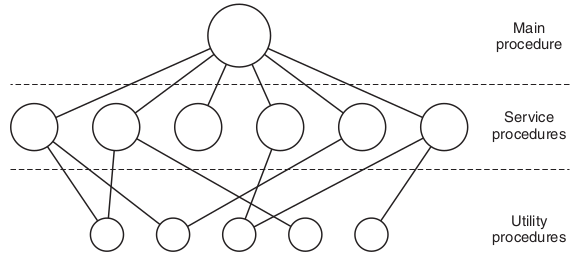
\includegraphics[width=0.75\textwidth]{FIG/1-24.png}
	   \caption{简单的单体系统结构模型} \label{fig:monolithic}
   \end{figure}
   	
   除了在计算机启动的时候加载核心操作系统之外,许多操作系统支持可加载的扩展模块,像I/O设备驱动和文件系统,这些组件是按需加载的。在UNIX中它们被称为共享库(shared library),在Windows中它们被称为动态链接库(Dynamic Link Library,DDL)。它们的文件扩展名为ddl,在\texttt{C:$\backslash$Windows$\backslash$system32}目录下有1000多个系统调用。
   
   \subsection{分层系统}
   
   把图 \ref{fig:monolithic} 中的结构进一步通用化,就形成了一个层次式结构的操作系统,它的上层软件都是基于下一层软件的基础之上构建的。E. W. Dijkstra (1968)和他的学生在荷兰的Eindhoven技术学院所开发的THE系统是第一个按照此结构构建的操作系统。THE系统是为一种荷兰的计算机Electrologica X8设计的一种简单的批处理系统,其内存只有32K个字,每个字有27位(那时二进制位是非常昂贵的)。
   
   如图 \ref{fig:layered} 所示,这个系统分为6层。第0层进行处理器分配,在中断发生或计时器过期时在进程之间切换。在第0层之上,系统由一些连续的进程组成,每一个进程都可以被编程而不用担心多个进程运行在一个处理器上的事实。也就是说,第0层提供了基本的CPU多道程序设计功能。
	
   \begin{figure}[ht]\small
		\centering
		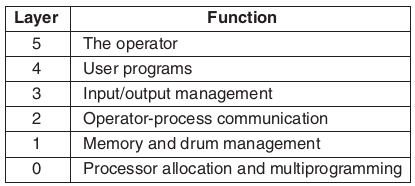
\includegraphics[width=0.75\textwidth]{FIG/1-25.png}
		\caption{THE操作系统的结构} \label{fig:layered}
   \end{figure}

	第一层是内存管理。它在主存中为进程分配内存,当内存用完时在一个512字节的磁鼓上保留进程的一部分页面。在第一层之上,不需要担心进程是在内存中还是在磁鼓上运行,第一层的软件保证一旦需要某一个页面,该页面必定已在内存中,并在页面不需要的时候将其移出。第2层处理进程和操作员控制台(即用户)之间的通信。第3层负责管理I/O设备,并对进出它们的信息流进行缓冲。第4层是用户程序层,他们不需要担心进程,内存,控制台或者I/O管理。系统操作员进程位于第5层中。在MULTICS中采用了更进一步的通用层次化概念,与分层不同的是,MULTICS被描述为一组同心圆,内部的圆比外部的圆拥有更高的优先权限(他们实际上是一样的)。当一个外环的过程调用内环的过程的时候,它必须执行一条等价于TRAP的指令,在执行该指令前,要进行严格的参数合法性检查。在MULTICS中,虽然整个操作系统是每个用户进程地址空间的一部分,但硬件使得能够指定单个过程(实际上是内存段)以防读、写或执行。尽管THE的分层方案只是一个设计上的辅助,因为在MULTICS中所有的部分都链接成一个可执行的程序,环机制在运行时非常常见并且由硬件强制执行。环形机制的好处是它可以轻易地扩展成用户子程序。例如,一个教授可以在第n环中设计给学生的考试程序并打分,而学生程序运行在第n+1环,这样的话他们就不可以改变他们的分数。
	
	\subsection{微内核}
	
	在分层的方法中,设计者有一个选择在哪里甚至内核态与用户态的边界。传统地说,所有的层次是运行在内核中的,但是它不是必须的。事实上,一个强有力的理由是尽可能少地使用内核模式,因为内核中的一个错误可以使得程序立即崩溃。相反的是,可以将用户进程设置为较小的权限,这样某个错误的后果也将不是致命的。不同的研究者已经研究了每1000行代码中bug的数量(e.g., Basilli and Perricone, 1984; and Ostrand and Weyuker, 2002)。Bug的密度取决于模块大小,模块的使用年限,对于商用工业系统而言,一个大约的数字是每1000行代码中有2-10个bug。
	这就意味着一个有着500万行代码的单体操作系统中,大约会有10000-50000个内核错误。当然,并不是所有的错误都是致命的。比如给出了不正确的故障错误信息等错误,实际上是很少发生的。不管怎么样,计算机是充满着大量的错误的,所以计算机的制造商设置了复位按钮(通常是在面板的前面)。而电视机,立体音箱和汽车的制造商却不这么做,尽管这些装置中也包含着大量的软件。
	微内核设计的一个基本想法是通过将操作系统分割成为小的,良好定义的模块来实现高可用性,只有其中的一个模块-微内核-运行在内核态,其余的模块由于功能相对弱一些,则作为普通用户程序运行。特别地,通过运行每一个设备驱动和文件系统作为一个独立的用户进程,如果一个bug出现,会导致这个组件失败,但是不会导致整个系统的崩溃。因此,音频驱动器中的一个bug将会导致声音断续或停止,但是不会使得电脑崩溃。相反,在单体系统中,所有的设备驱动都是在内核态中的,一个有bug的音频驱动程序很容易地引发对无效地址的引用,从而造成恼人的系统立即停机。
	许多微内核系统已经被实现和应用了数十年(Haertig et al., 1997; Heiser et al., 2006; Herder et al., 2006; Hildebrand, 1992; Kirsch et	al., 2005; Liedtke, 1993, 1995, 1996; Pike et al., 1992; and Zuberi et al., 1999)。除了基于Mach微内核的OS X之外,通常的桌面操作系统并不使用微内核。然而,它们在实时系统,工业系统,航空系统和军事应用中用地却非常广泛,这些领域都是关键任务,有很高的可靠性要求。知名的微内核有Integrity,K42,L4,PikeOS,QNX,Symbian,和
	MINIX 3。我们在这里简要地介绍一下MINIX 3,该操作系统把模块化的思想推向了极致,它将大部分的操作系统分解成许多独立的用户态进程。
	MINIX 3是一个POSIX兼容的,完全开源的操作系统,并且可以在www.minix3.org获得免费的开源源代码(Giuffrida et al., 2012; Giuffrida et al., 2013; Herder et al., 2006; Herder et al., 2009; and Hruby et al., 2013)。
	MINIX3微内核大约只有12000行C代码和1400行用于底层功能实现的汇编代码,如获取中断,切换进程等。C代码管理和调度进程,处理进程间通信(通过在进程间进行消息传递),提供大约40个内核调用,它们使得操作系统的其他部分可以完成其工作。这些调用完成诸如连接中断句柄,在地址空间中移动数据以及为新创建的进程安装新的内存镜像等功能。MINIX3的进程结构如图 \ref{fig:minix3} 所示,其内核调用句柄用\texttt{Sys}表示。时钟设备驱动也在内核中,因为这个驱动和调度器交互密切。所有的其他设备驱动都做为单独的用户进程进行。
	
    \begin{figure}[ht]\small
		\centering
		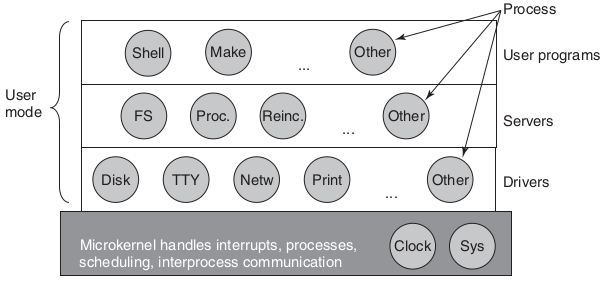
\includegraphics[width=0.75\textwidth]{FIG/1-26.png}
		\caption{MINIX3操作系统的结构} \label{fig:minix3}
	\end{figure}
	
	在内核的外部,系统的构造有三层进程,他们都在用户态运行。最底层包括设备驱动,因为它们运行在用户态,他们没有对I/O端口空间的物理地址,不能够直接执行I/O指令。相反地,为了编程一个I/O设备,驱动器构建一个结构,告诉向哪个I/O接口中设置什么值,并进行一个内核调用告诉内核去写。这种方法意味着内核可以检查驱动程序是否正在从它被授权使用的I/O中写入(或读取)。因此(与单片设计不同的是),一个有缺陷的音频驱动程序不会意外地写磁盘。在驱动层之上是另一个包含服务的用户模式层,它承担了操作系统大部分的工作。一个或多个文件服务器管理文件系统,进程管理器创建,销毁和管理进程。用户程序通过向服务器发送短消息请求POSIX系统调用来获得操作系统服务。例如,需要进行读取的进程向其中一个文件服务器发送一条消息,告诉它要读取什么。一个有趣的服务器是再生服务器(reincarnation server)。它的工作是检查其他的服务器和驱动是否在正确地工作。在这个过程中,如果发现一个有错误的,它将会被自动地被替换,而无须任何用户的参与。这种方式使得系统具有自修复能力,并且获得了较高的可靠性。系统有很多的方法来限制进程的权限。像前面提到的,驱动程序只能触及授权的I/O端口,对内核调用的访问也是按照单个进程控制的。这是考虑到进程具有向其他多个进程发送消息的能力。进程还可以授予其他进程有限的权限内核访问它们的地址空间。
	例如,一个文件系统可以给磁盘驱动器有限的许可,让内核在文件系统地址空间的固定位置进行对盘块的读入工作。总体来说,所有的这些限制都是为了让每一个驱动程序和服务器只拥有完成其工作的权限,这就大大限制了故障部件可能造成的危害。
	一个与小内核相关联的思想是内核中机制与策略相分离的原则。为了更清晰地明白这一点,让我们考虑一下进程调度。一个相对简单的调度算法是给每一个进程赋予一个数字优先权,内核运行拥有最高权限的进程。在这里,机制(在内核中)就是找到最高优先权的进程并运行之。而策略,给每一个进程分配优先级,则可以在用户态进行。在这种方式下,策略和机制可以分离,进而可以使得内核更小。
	
	\subsection{客户端-服务器模式}
	
	一个微内核思想的略微变体是将进程分为两类,一类是提供服务的进程,称为服务器,一类是使用这些服务的进程,称为客户端。这个模式就是所谓的服务器-客户端模式。通常最底层是一个微内核,但是不是必须的,其本质是存在服务器进程和客户端进程。客户端进程和服务器进程之间的通信主要通过消息传递。为了获取一个服务,一个客户端进程构建一个它想要什么的消息并把它发给合适的服务。服务接着进行具体的工作并将结果返回。如果客户端和服务器正好是运行在同一台机器上,可以进行一定的优化,但是概念上说,这里讨论的还是消息传递。
	这个思想一个显然的普遍模式是,客户端和服务器运行在不同的计算机上,他们通过局域网或者广域网连接,像图 \ref{fig:client-server} 所示的那样。
	
    \begin{figure}[ht]\small
		\centering
		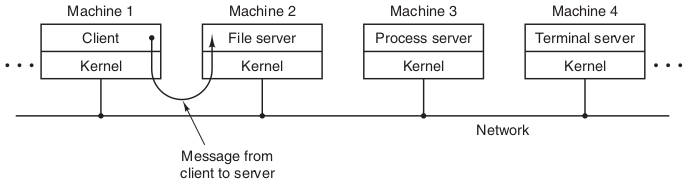
\includegraphics[width=0.75\textwidth]{FIG/1-27.png}
		\caption{一个位于网络上的客户端-服务器模式} \label{fig:client-server}
	\end{figure}

	因为客户端是通过发送消息和服务器进行通信的,所以客户端其实并不需要知道消息是否在它所在的本地机器进行处理或者是通过网络发送给一个远程的机器。对于客户端而言,这两种请求是一样的:都是发送请求并得到回应。所以,客户端-服务器模式是一种可以应用在单个机器或者一组网络机器的抽象。许多系统,包括用户家里的PC,都成为客户端,在别处运行的大型机器为服务器。事实上,许多Web就是以这个方式运行的。一台PC像一台服务器发送一个网页的请求,服务器返回网页请求。这是一个网络中客户端-服务器模式的典型应用方式。

	\subsection{虚拟机}
	
	OS/360系统最初是一个严格的批处理系统。许多360的用户希望能够在终端上交互工作,所以不同的组,包括IBM内部和外部的,决定为360写一个分时复用系统。后来推出了正式的IBM分时系统TSS/360,但是它非常庞大,运行缓慢,在花费了近5000万美元的研发费用之后还是被弃用了。但是在麻省剑桥的IBM科学研究中心的小组,开发了另一个完全不同的系统,该系统最终被IBM接受为产品。它的直接后代,称为z/VM,目前被IBM广泛地应用于大型机上,例如,zSeries在大型企业数据中心中被大量使用,例如,作为电子商务服务器,每秒处理数百或数千个事务,并使用大小达数百万GB的数据库。
	
	\textbf{VM370}
	
	这个系统,一开始叫做CP/CMS,后来重新命名为VM/370。它是源于一个机敏的观察,即分时系统应该提供这些功能:(1)多道程序 (2) 一个比裸设备带有更方便接口的扩展机器。VM/370的实质是分离这两个功能。系统的核心,被称为虚拟机监视器(VMM),运行在裸设备之上并且进行多道程序设计,向上层提供不是一个而是若干台虚拟机,像图 \ref{fig:vm370} 所示的一样。
	
    \begin{figure}[ht]\small
		\centering
		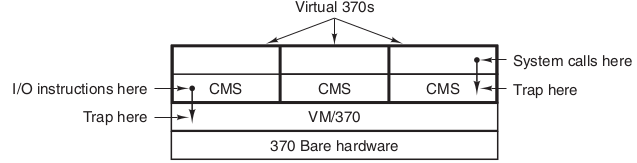
\includegraphics[width=0.75\textwidth]{FIG/1-28.png}
		\caption{配有CMS的VM370结构} \label{fig:vm370}
	\end{figure}

	然而,和其他操作系统不同的是,这些虚拟机并不是具有文件以及其他特征的扩展的机器,与之相反,它们是裸机硬件的完美复制品,包括内核态/用户态,I/O,中断以及一些其他硬件所具备的所有其他功能。因为每一个虚拟机和真实的硬件是类似的,每一个都可以运行直接在裸露机器上运行的任何操作系统。不同的虚拟机可以运行不同的操作系统,而且往往就是如此。在原始的IBM VM/370系统上,一些运行OS/360系统或者其他大型批处理和事务处理操作系统,其他运行单用户,交互式系统供分时用户使用,这个系统称为会话监控系统(Conversational Monitor System),后者在程序员中很流行。当一个CMS程序执行系统调用的时候,系统调用陷入到虚拟机自己的操作系统中,而不是VM/370系统上。好像它运行在一个真实的机器上而不是虚拟机上。CMS接着发出普通的硬件I/O指令读取它的虚拟磁盘或者它需要的任何其他东西来执行系统调用。这些I/O指令被VM/370陷入,然后,作为对实际硬件模拟的一部分,VM/370完成指令。通过完全分离多道程序功能和提供机器两者的完全分离,每个部分都变得更加地简单,更加地灵活和易于维护。虚拟机的现代化身z/VM通常是运行多个完整的操作系统而不是运行简化成像CMS那样的单用户系统。例如,zSeries有能力和IBM的操作系统一起,运行一个或多个Linux操作系统。
	
	\section{虚拟机的再次发现}
	
	IBM拥有虚拟机产品已经有40年了,一些其他的公司,包括Oracle,HP公司,在它们的高端服务器产品中增加了虚拟机的支持,而在PC上,虚拟机的思想直到最近以前一直被忽视了。但是在过去的一些年中,新的需求,新的软件,新的技术使得虚拟机又成为一个热点。首先是需求。许多公司将他们的邮件服务器,Web服务器,FTP服务器以及一些其他的服务器放在不同的计算机上,有时候使用不同的操作系统。他们把虚拟机看作是将这些服务放在同一台机器上而不用担心其中的一个服务崩溃影响到其他的服务。虚拟化在Web托管世界里也很流行。没有虚拟化,Web托管客户端只能在共享托管(这只是给他们一个在Web服务器上的登录账户,而对服务器的软件没有控制权)和直接托管(给它们自己的机器,这个方法非常地灵活,但是对于小型和中型的网站而言,成本效益比不高)之间进行选择。当Web托管公司提供租用的虚拟机时,一台物理机器就可以运行好多台虚拟机,而每一台虚拟机都可以看做是一个独立的机器。租用虚拟机的客户可以运行他们想要运行的任何操作系统和软件,但是只需要支付独占一台机器几分之一的费用(因为一台物理机器可以同时支持多台虚拟机)。虚拟化的另一个作用是给那些想在一台机器上运行一个或多个操作系统的终端用户使用,像Windows和Linux,因为他们最喜欢的程序包有的运行在这个操作系统上有的运行在那个操作系统上。这种情形就像图 \ref{fig:hypervisor} (a)所示的那样,在这里
	术语"虚拟机监视器"已经被重新命名为第一类虚拟机管理程序(type 1 hypervisor),这个名称现在更常用因为"Virtual  Machine Monitor"已经超出了人们可以承受的最大按键次数。但是请注意,许多作者可以互换使用这些术语。
	
    \begin{figure}[ht]\small
		\centering
		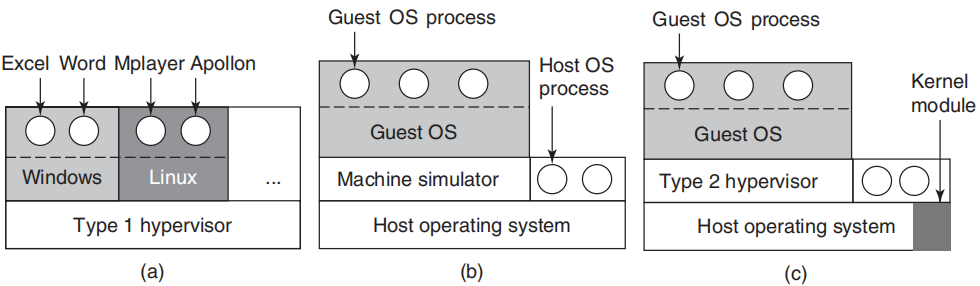
\includegraphics[width=0.75\textwidth]{FIG/1-29.png}
		\caption{a).第一类虚拟机管理程序 b).理论上的第二类虚拟机管理程序 c).实际上的第二类虚拟机管理程序} \label{fig:hypervisor}
	\end{figure}
	
	尽管没有人怀疑虚拟机的吸引力,但是问题是如何实现。为了能在一台计算机上运行虚拟机,它的CPU必须可以虚拟化。简而言之,问题就在这里。当一个运行在虚拟机上的操作系统执行一个优先权指令的时候,像修改PSW和执行I/O。必须将硬件陷阱设置到虚拟机监视器上,这样才能在软件中模拟指令。在一些CPU上(特别是Pentinum和它的后继者及克隆版中)试图在用户态执行特权指令时,会被忽略掉。这种属性使得在这个硬件上无法使用虚拟机,这也解释了PC世界对虚拟机不感兴趣的原因所在。但是也有一些Pentinum的解释器,比如Bochs,但是这种解释器会带来1-2个数量级上的性能损失,在一些要求高的工作场合失去了实际的应用价值。然而,这种情况在上世纪90年代末和本世纪初期因为一些学术研究工程的开展而改变,特别是斯坦福的Disco,剑桥大学的Xen,这些研究论文导致了一些商业产品的诞生(VMWare Work Station和Xen)和对虚拟机研究兴趣的重新滋生。除了VMWare和Xen,现在流行的虚拟机还有KVM(为Linux内核而建的),Virtual Box(由Oracle开发)和Hyper-V(由Microsoft开发)。
	这些早期的研究工程通过在线翻译代码块改善了类似Bochs之类的解释器的性能,并把它们保存在内部的Cache中,并在它们执行的时候重新使用它们。这在一定程度上改善了性能,也导致了我们称为机器模拟器的诞生,像图 \ref{fig:hypervisor}(b) 所示的那样。尽管这项被称为二进制翻译的技术对改善性能起到了一定的作用,其结果也足够优秀在学术会议上发表论文,但是这在十分重视性能的商业环境中还是远远不够的。
	下一个改善性能的步骤是加入一个添加分担重担的内核模块,像图 \ref{fig:hypervisor}(c) 所示的那样。在现实中,所有的商用的虚拟机,像VMWare Work Station,使用混合策略(当然也有许多其他的改进)。它们被称为类型2虚拟机,所以我们将在本书中沿用此称谓,甚至我们更倾向于称它类型1.7虚拟机来反映其并不完全是用户态程序的事实。在第7章中,我们将具体地描述VMWare Work Station是如何工作的,以及各部分的作用。
	实际上,类型1虚拟机和类型2虚拟机的真正区别是,类型2使用一个宿主操作系统以及它的文件系统来创建进程,存储文件等。而类型1虚拟机没有类似的底层支持,必须自己做这些功能。当类型2的虚拟机启动后,它读取客户操作系统所安装的CD-ROM(或者CD-ROM镜像文件),并将客户操作系统安装在一个虚拟磁盘上,它只是宿主操作系统的文件系统中一个巨大的文件。类型1虚拟机不能做这个是因为它没有宿主操作系统来存储文件
	。它们必须在一个原始的磁盘分区上自己做存储管理。当客户机操作系统被启动后,它做的事情和在真实的硬件上做的事情是一样的,典型的动作是启动一些后台进程进而启动GUI图形用户界面。对于用户,客户机操作系统表现地像它做裸金属设备上表现得一样,尽管实际是已经不是那么回事了。处理控制指令的另外一个方法是修改操作系统并移除它们,这个方法不是真正的虚拟化,而是半虚拟化。我们将在第7章中详细讨论虚拟化。
	
	\textbf{Java虚拟机}
	
	虚拟机使用的另外一个领域,但是又有所不同的是用于Java程序。当SUN公司发明了Java编程语言,它也发明了一个叫做Java虚拟机(Java Virtual Machine)的虚拟机(一种计算机体系结构)。Java编译器为JVM产生代码,这些代码接着被Java解释器的软件执行。这个方法的好处是JVM的代码可以通过网络传递到任何一台有Java解释器的机器上并在那里执行。如果编译器产生了SPARC或者X86的二进制程序,他们就不能随便被传播到哪里并运行了(当然,SUN公司也生产了一个产生SPARC二进制程序的编译器和一个分布式的SPARC解释器,但是JVM是一个简单很多的解释器架构)。使用JVM的另外一个好处是,如果解释器被正确地实现(当然这可不是一件小事),还要对JVM程序进行安全性检查,并在一个受保护的环境中执行,这样程序就不能盗取数据和做其他有害的操作了。
	
	\subsection{外核}
	
	和虚拟机克隆真实的机器不同,另一个策略是对其进行分区,换句话说,给每一个用户一个资源的子集。这个一个虚拟机可能会获得第0到1023个磁盘块,第二个虚拟机获取第1024到2047个磁盘块,以此类推。
	在底层,运行在内核态的,是一个被称为外核的应用程序。它的工作是为每一个虚拟机分配资源,并检查使用这些资源的企图,以确保没有别的虚拟机想要用其他虚拟机的资源。每一个用户级的虚拟机都可以运行它自己的操作系统,如VM/360和虚拟的奔腾8086,除非每一个已经被严格限制了只能使用为他分配的,他自己的资源。外核机制的另外一个好处是它节省了一层映射层。在其他的设计中,每一个虚拟机只考虑它自己的磁盘,数据块从0到一个最大值,所以虚拟机监控器必须维持一个重新映射磁盘地址的表格。而外核方案,就不需要这样。外核仅仅只需要记录哪一个虚拟机被分配到哪一个资源上了。这个方法仍然有可以分离多道程序(在外核中)和用户操作系统代码(在用户态)的好处,但是代价更小,外核所做仅仅是保证各个虚拟机不发生冲突。
	
	\section{依靠C语言的世界}
	
	操作系统通常是一个由很多编程者共同开发和很多模块的大型C(或者C++)程序。开发操作系统的环境和写Java小程序的环境是非常不同的。这个小节试图给有时候编写Java和Python程序的编程者介绍一下编写操作系统的环境。
	
	\subsection{C语言}

	这不是一个C语言的说明文档,而是介绍C语言和类似Python,特别是Java语言的一些关键不同之处。Java是基于C语言的,所以这两者有非常多的相似之处。为了方便起见,我们聚焦于Java。Java,Python和C都是命令式语言,有数据类型,变量和控制语句,例如,C语言中原始的数据类型是整型(包括长整型和短整型),字符型和浮点数。复合的数据结构可以使用数组,结构体和联合体。C语言中的控制语言和Java中的也非常类似,包括if,switch,for,while语句等。两种语言的函数和参数形式基本相同。C语言有的但是Java和Python没有的特征是显式指针。指针是指向变量(包括地址)或者数据结构的变量。考虑一下下面的语句:
	char c1, c2, * p;
	c1 = ’c’;
	p = \&c1;
	c2 = * p;
	以上语句声明了c1,c2两个字符变量,和一个指向字符变量的指针,第一个赋值语句将字符'c'的ASCII码存放在变量c1中,第二条语句将c1的地址赋值给指针变量p,第三条语句是将指向指针p的变量内容赋值给变量c2,所以这些语句执行以后,c2也包含了'c'的ASCII码。理论上,指针是类型化的,因此不应该将浮点数的地址分配给字符指针,但是实际的编译器接受这样的赋值,尽管有时候会发出警告。指针是一种非常强大的结构,但是如果使用不当,会是很多错误发生的根源。
	C语言没有的一些特征,包括内联字符串,线程,包,类,对象,类型安全和垃圾回收。最后一个是操作系统的"淋浴器塞子"。C语言中的存储都是编程人员静态或者显式分配和回收的,通常使用库函数\texttt{malloc}和\texttt{free}。正是由于后面的特性,由程序员完全操作内存-通过显式的指针,使得C语言对编写操作系统而言非常具有吸引力。操作系统在一定程度上是实时的系统,即使通用的操作系统也是这样。当中断发生的时候,操作系统通常只有若干微秒去处理发生的情况,否则就会有关键信息丢失,而且在任意时刻启动垃圾回收功能是不可接受的。
	
	\subsection{头文件}
	
	一个操作系统工程通常包括一定数量的目录,每一个都包含许多的c文件,这些文件存有系统某些部分的源代码,还有一些.h的头文件,包含被一个或多个源文件使用的声明和定义。头文件还可以包含一些简单的宏定义,像:\#define BUFFER\_SIZE 4096。
	允许编程者定义声明一些常量,所以当在代码中使用BUFFER\_SIZE变量的时候,它在编译的时候会被替换成数字4096。好的C语言编程习惯是对除了0,-1和1之外的变量进行命名,有时候甚至对0,-1和1进行命名。宏还可以带参数,例如: \#define max(a, b) (a > b ? a : b),允许编程者写i = max(j, k+1)和i = (j > k+1 ? j : k+1)来在i中存储j和k+1之间较大的一个。头文件还可以包含条件编译:
	\\\indent \#ifdef X86 
	\\\indent\indent  intel\_int\_ack(); 
	\\\indent \#endif
	\par 将会编译函数intel\_int\_ack()如果X86宏被定义的话,如果没有被定义的话则不编译。条件编译经常用来分离体系架构相关的代码,这样只有系统在X86体系结构上编译时才可以插入特定的代码,而其他的一些代码只有在SPARC架构下编译的时候才会被编译,等等。一个C文件,可以在头部使用\#include指令包含0个头文件和更多的头文件。也有很多和普通的c文件一样的头文件被存放在特定的目录下。
	
	\subsection{大型编程项目}
	
	为了构建操作系统,每一个c文件都被编译器编译成一个.o文件。后缀名为.o的目标文件包含着目标机器的二进制指令。它们稍后将会直接被CPU执行,在C语言的世界里,没有像Java和Python一样的字节码。C编译器的第一道是C预处理器。它读取每一个.c文件,每次遇到\#include指令的时候,它就将相应的头文件取来,并进行处理,扩展宏,处理条件编译(以及其他的事务),并且把结果传递给编译器的下一道,好像它们原先就包含这些头文件似的。因为操作系统非常地庞大(通常500万行代码是很正常的),当每次改变一个文件就需要对所有的东西进行重新编译是不可以接受的。另外一方面,改变一个被上千个其他文件包含的关键的头文件则确实需要重新编译这些文件。跟踪哪一个文件依赖于哪一个头文件在没有帮助的情况下是完全不可行的。幸运的是,计算机非常善于处理事物的分类。在UNIX系统中,有一个称为make的程序(还有一些其他的变种,如gmake,pmake等)来读取Makefile,告诉哪些文件依赖于哪些其他的文件。make要做的事情是检查为了构建操作系统二进制程序需要哪些目标文件,并且检查这些所依赖的文件(源代码和目标文件)是否在上一次被编译后被修改后,如果是,目标文件将需要被重新编译。当make程序需要决定重新编译哪一个c文件的时候,它就会触发c编译器来重新编译它们,进而将需要重新编译的文件降低到最少。在一些大型的工程中,创建makefile是一件非常容易出错的事情,但是现在已经有工具可以自动地做这件事了。当所有的.o文件都准备好了以后,它们被传递到一个叫做连接器的程序,来将它们组合成一个单个的可执行二进制文件。此时还包括调用的任何库函数,解析函数间引用,并根据需要重新定位主机地址。当连接器结束的时候,结果是一个可执行的程序,在UNIX系统中通常称为a.out程序。图 \ref{fig:compile} 给出了一个程序进程的不同组成部分,包括3个C程序和2个头文件。尽管我们在这里是讨论操作系统的开发,这些也都可以应用于任何一个大型的程序。
		
	\begin{figure}[ht]\small
		\centering
		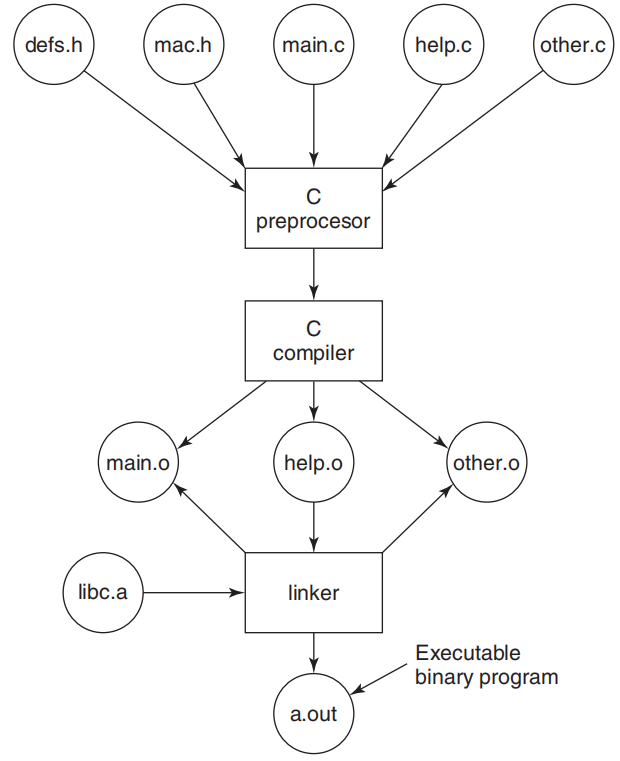
\includegraphics[width=0.75\textwidth]{FIG/1-30.png}
		\caption{编译一个C程序和头文件使得其可以运行的过程} \label{fig:compile}
	\end{figure}
	
	\subsection{运行时模型}
	
	当操作系统的二进制文件被链接的时候,计算机可以重启而且新的操作系统可以启动了。一旦运行,它可以动态地加载没有被静态地加载进来的操作系统部分,像设备驱动和文件系统。在运行时操作系统可以包括多个片段,像代码段,数据段和栈。代码段通常是不可改变的,在执行中不被改变。数据段从一定的大小开始,并用一些值进行初始化,但是它可以根据需要进行改变。栈一开始是空的,但是随着函数的调用和返回,栈开始增长和收缩。通常代码段被放置在接近内存的底部,数据段紧跟着在其之上,并且可以向上增长。栈段在高的虚拟地址,并且可以向下增长,但是不同的系统工作起来也不相同。在所有的情况下,操作系统的代码都是被硬件直接执行的,没有解释器和实时编译,这一点和Java很不相同。
	
	\section{操作系统的研究}
	
	计算机科学是一个高速发展的领域,很难预言它将会朝什么方向发展。在大学和工业界研究性质的实验室里的研究者们不断地想出新的想法,这些想法有一些变得不知所踪,而有一些则成为未来产品的基石,并且对工业界和用户产生了重要的影响。事后告诉哪些会怎样哪些会怎样总是比实时地告诉更加容易一些。而且分离小麦和麸糠是特别困难的因为它通常要花费20-30年才能将一个想法变为现实并且产生影响。例如,当美国总统埃森豪威尔在1958年设立国防部高级研究计划署的时候,他试图通过五角大楼的国防预算来试图阻止陆军对海军和空军的削弱,他不是试图发明互联网。但是APRA做的其中一件事情是资助一些大学研究研究在当时看来很荒诞的概念-包交换,这导致了第一个实验性包交换网络的诞生-ARPANET。它在1969年启用了。不久,APRA资助的其他网络和ARPANET也连接到了一起,于是因特网诞生了。于是因特网被学术研究者很高兴地用来收发邮件长达20年之久。在1990年代早期,蒂姆·伯纳斯·李在日内瓦的CERN的研究中心实验室发明了万维网,马克·安德森在伊利诺伊大学为其写了一个图形化的浏览器。突然之间,互联网上充满了年轻人的聊天,埃森豪威尔总统可能在他的坟墓里翻身了。操作系统的研究同样会导致实际的系统发生很大的变化。正如我们之前提到的那样,第一代的商用计算机系统都是批处理系统,直到M.I.T在1960年代发明了通用的分时系统。计算机在道格·恩格尔巴特发明鼠标之前都是基于文本的,在1960年代末期,斯坦福的研究机构发明了图形用户界面。在本节以及本书中可比较的其他章节中,我们将简要地回顾一下过去的5到10年之间操作系统领域的一些研究,这是为了让读者了解可能会发生什么。这个介绍当然不是综合性的,主要是基于在操作系统领域的顶级研究会议上发表的论文,因为这些论文能够发表肯定是经历了非常严谨的同行评审。要注意到在计算机领域-和其他的研究领域有所不同的是-大部分的好的研究成果是发表在会议上的,而不是期刊上的。大部分在研究章节被引用的论文都是发表在ACM,IEEE和USENIX上的,并且通过网络向它的用户(包括学生用户)开放。要获得这些组织机构和它们的图书馆更多的信息,可以通过以下网站:	
	\\\indent ACM http://www.acm.org

	IEEE Computer Society http://www.computer.org

	USENIX http://www.usenix.org
	事实上,所有的操作系统研究者们意识到当前的操作系统是庞大的,复杂的,不可靠的,不安全的,充满了错误,并且某一个操作系统比其他操作系统有着更多的错误(在这里略去名字以免承担责任)。结果,就出现了大量的研究工作来探讨如果构建一个更好的操作系统。近年来的研究工作有以下一些:关于错误和调试(Renzelmann et al., 2012; Zhou et
al., 2012),故障恢复(Correia et al., 2012; Ma et al., 2013; Ongaro et al.,2011; Yeh Cheng, 2012),电源管理(Pathak et al., 2012; Petrucci Loques, 2012; Shen et al., 2013),文件和存储系统(Elnably, Wang, 2012; Nightingale et al., 2012; Zhang et al., 2013a),高性能I/O(De Bruijn et al., 2011; Li et al., 2013a; Rizzo, 2012),超线程和多线程(Liu et al., 2011),动态更新(Giuffrida et al., 2013),GPU管理(Rossbach et al., 2011),内存管理(Jantz et al., 2013;
Jeong et al., 2013),多核操作系统(Baumann et al., 2009; Kapritsos, 2012; Lachaize et al., 2012; Wentzlaff et al., 2012),操作系统正确性(Elphinstone et al., 2007; Yang et al., 2006; Klein et al., 2009),操作系统可靠性(Hruby et al., 2012; Ryzhyk et al., 2009, 2011 Zheng et al., 2012),隐私与安全(Dunn et al., 2012; Giuffrida et al., 2012; Li et al.,
2013b; Lorch et al., 2013; Ortolani Crispo, 2012; Slowinska et al., 2012; Ur et al., 2012),用户和性能监控(Harter et. al, 2012; Ravindranath et al., 2012)和虚拟化(Agesen et al., 2012; Ben-Yehuda et al.,
2010; Colp et al., 2011; Dai et al., 2013; Tarasov et al., 2013; Williams et al.,2012)以及一些其他的许多主题。
	
	\section{本书剩余部分的结构}
	
	我们已经介绍了操作系统并且对操作系统形成了一个总体的概览。现在是时候开始深入到细节了。像已经提到的那样,从编程者的角度看,操作系统的主要目的是提供一些关键的抽象,其中最重要的是进程和线程,地址空间和文件。接下来的三章会集中讨论这些关键部分。
	
	第二章是关于进程和线程,讨论它们的属性以及它们之间是如何通信的,也给出了几个进程间通信是如何工作和如何避免陷阱的详细例子。
	第三章我们将详细学习地址空间和它的附属物:内存管理。将会讨论到虚拟内存这个重要的主题,以及一些紧密相关的概念,分页和分段等。
	第四章我们将讨论对所有都很重要的主题:文件系统。在相当的程度上,大部分情况下用户看到的是文件系统。我们将同时关注文件系统的接口和文件系统的实现。
	第五章是输入/输出系统。设备独立性和设备依赖性的概念将会被关注。一些重要的设备,包括磁盘,键盘,显示器等,将会被作为例子使用到。
	第六章是关于死锁。我们将在本章简要地展示什么是死锁,还有一些其他的更多内容,比如如何避免和预防死锁等。
	到了这里,我们将完成一个单CPU操作系统基本原则的学习。但是还有更多的内容需要讨论,特别是一些高级的主题。在第7章中,我们将讨论虚拟化。我们将同时讨论虚拟化的原则以及一些现有的虚拟化解决方案的例子。因为虚拟化在云计算中使用地很多,我们还将关注现有的云。另外一个高级主题是多处理器系统,包括多核,并行计算机和分布式系统。这些主题将在第8章中覆盖到。
	操作系统中一个非常重要的主题是安全,将在第9章中讨论。在该章将被讨论到的主题是:威胁(病毒和蠕虫),保护机制和安全模型。
	接下来我们将学习一些实际的操作系统按列,包括UNIX,Linux,Android(第10章)和Windows 8(第11章)。我们将在第12章介绍一些操作系统设计方面的智慧与思想。
	
	\section{公制单位}
	
	为了避免任何的混乱,值得我们在本书中显式地声明,为了计算机科学的通用性,使用公制单位代替传统的英制单位(the furlong-stone-fortnight system)使用。图 \ref{fig:metric-prefixes} 给出了主要公制前缀。前缀主要是缩写成它的首字母。凡是单位大于1的首字母都大写。这样,1TB的数据库占据$10^{2}$字节的存储,100 psec(100 ps)时钟每$10^{-10}$秒滴答一次。因为\texttt{milli}和\texttt{micro}都是字母'm'开头,所以必须要对这两者作出区分。通常用'm'表示\texttt{milli},用 \textmu(希腊字母)表示\texttt{micro}。
		
	\begin{figure}[ht]\small
		\centering
		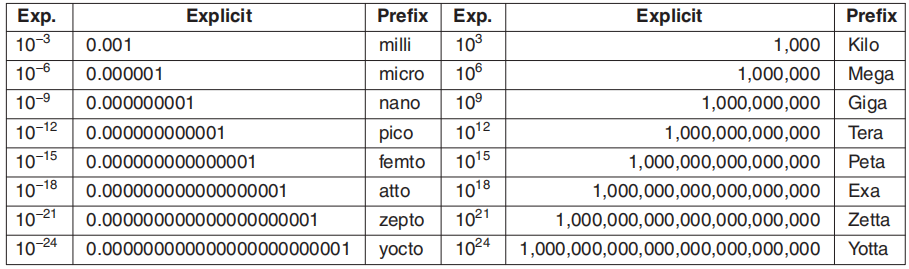
\includegraphics[width=0.85\textwidth]{FIG/1-31.png}
		\caption{主要的公制前缀}\label{fig:metric-prefixes}
	\end{figure}

	同时值得指出的是,在通常的工业实践中,测量存储容量大小的单位略微有所不同。如Kilo表示的$2^{10}$(1024)而不是1000,因为存储容量总是2的幂次方。因此1KB内存包含1024个字节,而不是1000个字节。相似地,1MB内存包含$2^{20}$(1,048,576)字节,1GB内存包含$2^{30}$(1,073,741,824)字节。但是,一条1-Kbps的通信线每秒传输1000比特,一个10-Mbps的局域网以每秒10,000,000位的速度运行,因为速度不是2的整数次幂。不幸的是,许多人会把这两个系统弄混淆,特别是磁盘的大小。为了避免混淆,我们在本书中使用KB,MB,GB表示$2^{10}$,$2^{20}$,$2^{30}$字节,而使用Kbps,Mbps和Gbps分别表示$10^{3}$,$10^{6}$和$10^{9}$bits每秒。
	
	\section{总结}
	
	操作系统可以从两个视角进行审视:资源管理者和扩展的机器。从资源管理者的角度,操作系统的工作是将系统的不同部分有效地管理起来。在扩展机器视角,操作系统的工作是提供用户比真实机器更加方便的抽象。这些包括进程,地址空间和文件。操作系统有很长的历史,从它们开始取代操作子开始,到现代的多道程序系统。亮点包括早期的批处理系统,多道程序系统和个人计算机系统。
	因为操作系统和硬件有很强的关联性,具备一些计算机硬件的知识将会有助于帮助理解它们。计算机是由处理器,内存和I/O设备组成的。这些部件通过总线连接。操作系统的基本概念就是基于进程,内存管理,文件系统,I/O管理和安全构成的。每一个部分都会在接下来的章节中依次讨论到。
	操作系统的核心是它可以处理的系统调用,这些将告诉操作系统真正如何使用。对于UNIX,我们看了四组系统调用,第一组系统调用是关于进程的创建和终止,第二组的是关于读写文件,第三组是关于目录管理,第四组则包括一些其他的系统调用。操作系统可以用多种方式进行组织,最常见的是单体系统,分层系统,微内核,客户机-服务器,虚拟机和外核。
	
	
	
	
	
	
	
	
	
	
	
	
	
	
	
	
	
	
	
	
	
	
	
	
	
	
	
	
	
	
	

	
	
	
	
	
	
	
	
	
	
	
	
	
	
	
	
	
	
	
	
	

%\setlength{\fboxrule}{0pt}\setlength{\fboxsep}{0cm}
%\noindent\shadowbox{
%\begin{tcolorbox}[arc=0mm,colback=lightblue,colframe=darkblue,title=学习目标与要求]
%\kai\textcolor{darkblue}{1.~~了解科学计算的一般过程.}\\
%\kai\textcolor{darkblue}{2.~~了解数值计算方法的研究内容和特点.}\\
%\kai\textcolor{darkblue}{3.~~理解数值计算误差的有关概念.}\\
%\kai\textcolor{darkblue}{4.~~掌握数值计算误差的控制方法.}
%\end{tcolorbox}}
%\setlength{\fboxrule}{1pt}\setlength{\fboxsep}{4pt}
%
%
%\section{Colored boxes}
%
%\begin{tcolorbox}[colback=red!5,colframe=red!75!black]
%  My box.
%\end{tcolorbox}
%
%\begin{tcolorbox}[colback=blue!5,colframe=blue!75!black,title=My title]
%  My box with my title.
%\end{tcolorbox}
%
%\begin{tcolorbox}[colback=green!5,colframe=green!75!black]
%  Upper part of my box.
%  \tcblower
%  Lower part of my box.
%\end{tcolorbox}
%
%\begin{tcolorbox}[colback=yellow!5,colframe=yellow!75!black,title=My title]
%  I can do this also with a title.
%  \tcblower
%  Lower part of my box.
%\end{tcolorbox}
%
%\begin{tcolorbox}[colback=yellow!10,colframe=red!75!black,lowerbox=invisible,
%  savelowerto=\jobname_ex.tex]
%  Now, we play hide and seek. Where is the lower part?
%  \tcblower
%  I'm invisible until you find me.
%\end{tcolorbox}
%
%\begin{tcolorbox}[colback=yellow!10,colframe=red!75!black,title=Here I am]
%  \input{\jobname_ex.tex}
%\end{tcolorbox}
%
%
%\begin{tcolorbox}[colback=blue!50,colframe=blue!25!black,coltext=yellow,
%    fontupper=\Large\bfseries,arc=6mm,boxrule=2mm,boxsep=5mm]
%  ofFunny settings.
%\end{tcolorbox}
%
%\subsection{\LaTeX-Table}
%
%\begin{table}[h]\begin{center}\color{darkblue}\caption{计算结果}\color{black}\label{tab1-2}
%{\footnotesize
%\begin{tabular}{r|r||r|r||r|r||r|r}\arrayrulecolor{darkblue}\hline\rowcolor{lightblue}
%  $n$&$I_n$&$n$&$I_n$&$n$&$I_n$&$n$&$I_n$\\\hline
%  19&0.008\ 3&14&0.011\ 2&9&0.016\ 9&4&0.034\ 3\\
%  18&0.008\ 9&13&0.012\ 0&8&0.018\ 8&3&0.043\ 1\\
%  17&0.009\ 3&12&0.013\ 0&7&0.021\ 2&2&0.058\ 0\\
%  16&0.009\ 9&11&0.014\ 1&6&0.024\ 3&1&0.088\ 4\\
%  15&0.010\ 5&10&0.015\ 4&5&0.028\ 5&0&0.182\ 3\\\hline
% \end{tabular}}\end{center}\end{table}
%
%
%\section{\LaTeX-Examples}
%
%\begin{tcblisting}{colback=red!5,colframe=red!75!black}
%This is a \LaTeX\ example:
%$\displaystyle\sum\limits_{i=1}^n i = \frac{n(n+1)}{2}$.
%\end{tcblisting}
%
%
%\section{Theorems}
%
%\begin{defi}{Summation of Numbers}{defi1.1}
%  For all natural number $n$ it holds:\\[2mm]
%  $\displaystyle\sum\limits_{i=1}^n i = \frac{n(n+1)}{2}$.
%\end{defi}
%
%\begin{theo}{Summation of Numbers}{theo1.1}
%  For all natural number $n$ it holds:\\[2mm]
%  $\displaystyle\sum\limits_{i=1}^n i = \frac{n(n+1)}{2}$.
%\end{theo}
%
%\begin{coro}{Summation of Numbers}{coro1.1}
%  For all natural number $n$ it holds:\\[2mm]
%  $\displaystyle\sum\limits_{i=1}^n i = \frac{n(n+1)}{2}$.
%\end{coro}
%We have given Theorem \ref{Theorem:theo1.1} on page \pageref{Theorem:theo1.1}.
%
%
%
%\begin{table}[h]\begin{center}\color{darkblue}\caption{计算结果}\color{black}\label{tab1-1}
%{\footnotesize
%\begin{tabular}{r|r||r|r||r|r||r|r}\arrayrulecolor{darkblue}\hline\rowcolor{lightblue}
%  $n$&$I_n$&$n$&$I_n$&$n$&$I_n$&$n$&$I_n$\\\hline
%  1&0.088\ 4&6&0.034\ 4&11&-31.392\ 5&16&9.814\ 5e+4\\
%  2&0.581\ 0&7&-0.029\ 0&12&157.045\ 7&17&-4.907\ 3e+5\\
%  3&0.043\ 1&8&0.270\ 1&13&-785.151\ 6&18&2.453\ 6e+6\\
%  4&0.347\ 0&9&-1.239\ 3&14&3.925\ 8e+3&19&-1.226\ 8e+7\\
%  5&0.026\ 5&10&0.296\ 7&15&-1.962\ 9e+4&20&6.134\ 1e+7\\\hline
%\end{tabular}}\end{center}\end{table}
%
%\section{graphicx}
%
%\begin{figure}[h]
%\begin{minipage}[t]{0.5\linewidth}
%\centering
%%\includegraphics[totalheight=1.2in]{fig/tu2-2}
%\caption{不动点迭代法收敛} \label{fig:tu2-2}
%\end{minipage}
%\begin{minipage}[t]{0.5\linewidth}
%\centering
%%\includegraphics[totalheight=1.3in]{fig/tu2-3}
%\caption{不动点迭代法发散} \label{fig:tu2-3}
%\end{minipage}
%\end{figure}
%
%
%
%\vspace{0.5cm}
%\addcontentsline{toc}{section}{\protect\numberline{}{习题一}}
%\markboth{习题一}{习题一} \centerline{\textcolor{darkblue}{\hei\zihao{4}
% 习题一}}\vspace{0.5cm}
%
%
        %第一章
\chapter{进程与线程}
\thispagestyle{empty}

	我们现在开始更加细节化地讨论操作系统是如何设计和构建的。对于任何操作系统而言,最核心的概念是:进程,一个正在运行的程序抽象。所有的其他事情都是基于这个概念的,操作系统的设计者(以及学生)应该尽快地了解什么是进程的概念。进程是操作系统提供的最古老和最重要的抽象。
	他们支持并发的多个操作即使在只有一个CPU的情况下。他们将一个CPU转化为多个虚拟的CPU。没有进程抽象,现代计算将不复存在。在本章中我们将深入探讨关于进程和线程的细节。
	
	\section{进程}
	
	所有的现代计算机都在同时做一个事情。人们之前使用计算机可能还没有充分意识到这个事实,所以再使用一些例子将这个情况讲清楚一些。首先考虑一个Web服务器,来自各地的请求都在请求网页。
	当一个请求来的时候,服务器检查是否将所需要的页面是否在cache中。如果是,则将其发回;如果不是,则启动一个磁盘请求去取它。但是,从CPU的角度来看,磁盘请求需要漫长的时间。当等待一个磁盘请求结束的时候,更多的请求可能会产生。如果有多个磁盘存在,一些或所有较新的磁盘可能在第一个请求得到满足之前就被发送到其他磁盘。很清楚,需要一些方法来建模和控制并发性。进程可以起到作用(特别是线程)。
	现在考虑一下用户的PC,当系统启动了以后,许多进程就无声无息地被启动了,尽管用户自己可能都不知道。例如,一个进程可能会被启动用来接收邮件。另外一个进程可能正在运行一个反病毒的程序,并且周期性地检查是否有新的病毒出现。除此之外,可能还有一些显式的进程,打印文件或者向USB驱动器中备份用户的照片,与此同时,用户可能还在网上进行冲浪。所有的这些活动都需要被管理,因此一个支持多线程的多道程序就来的非常及时了。在任何的多道程序系统中,CPU非常快速地从一个进程切换到另外一个进程,运行每一个进程数十或数百个微秒。但是,严格地说,在任何一个时候CPU都只能运行一个程序。在1秒钟之内,它可能对好几个进程产生作用,给人一种并行的错觉。有时候人们称之为伪并行策略,和真正的硬件并行的多核操作系统相比(有两个或者更多的CPU共享同样的内存)。跟踪并行的,多核的活动对于人来说是非常困难的。所以,操作系统的设计者们这些年开始提出了一种概念模型(顺序线程),使得并发性更容易被处理。它使用的这个模型,以及一些结果组成了本章的主要内容。
	
	\subsection{进程模型}
	
	在这个模型中,所有可以被运行的软件,有时候包括操作系统本身,都被组织成若干个顺序进程(Sequential process),简称进程。一个进程是一个正在执行的程序的实例,包括程序计数器现有的值,寄存器和变量。概念性地,每一个CPU都有一个自己的虚拟CPU。事实上,当然,真正的CPU在进程与进程之间来回地切换,但是为了理解好系统,想象一下一组进程在并行地执行比跟踪CPU是如何从一个程序向另外一个程序切换的要容易地多。这种快速的来回切换称为多道程序设计,如我们在第1章中提到的那样。
	在图 \ref{fig:processconcept} (a)中,我们看到一台计算机在内存中同时运行四个程序。在图 \ref{fig:processconcept} (b)中,我们看到四个进程,每一个都有自己的控制流程(它自己的逻辑程序计数器),而且每一个都是互相之间独立运行的。当然,只有一个物理的程序计数器,所以当每一个进程运行的时候,它们的逻辑程序计数器就会被加载到真正的程序计数器中。
	
	\begin{figure}[ht]\small
		\centering
		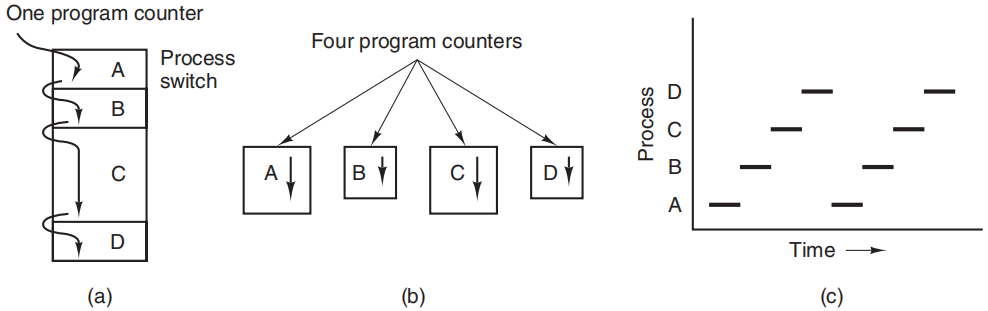
\includegraphics[width=0.85\textwidth]{FIG/2-1.png}
		\caption{a) 四个程序的多道程序 b) 四个独立的,顺序的概念模型 c) 只有一个程序在某一个时刻是活动的} \label{fig:processconcept}
	\end{figure}
	
	当程序结束的时候(时间到了),物理程序计数器保存在内存中的进程存储逻辑程序计数器中。从图 \ref{fig:processconcept} (c) 中我们可以看到,从一个足够长的时间间隔看,所有的进程都有进展,但是从一个给定的时间点来看,只有一个进程是实际运行的。在本章中,我们假设只有一个CPU。当然,逐渐这个假设就不为真了,因为新的芯片总是有多核的,有两个,四个,甚至更多的核。我们将在第8章中介绍多核芯片和多处理器。所以当我们说一个CPU一个时刻只能运行一个进程的时候,是指一个核心(一个CPU)在一个时刻只能运行一个进程。当CPU在进程之间来回切换的时候,一个进程执行其计算的速率将不一致,如果再次运行相同的进程,甚至可能无法再现以上的情形。所以,在对进程进行编程的时候,决不能对时序做任何想当然地假设。考虑一下,例如,一种播放音乐以伴随另一台设备运行的高质量视频的音频处理过程。
	因为音频一般会比视频稍微出现地晚一些,它向视频服务器发出信号开始播放,然后在回放音频之前运行一个空闲循环10000次。如果循环是一个可靠的计时器的话,一切都会变的OK,但是如果CPU决定在空闲循环的过程中切换到其他的线程,音频线程可能在相应的视频画面开始播放的时候还没有跟着播放出来,就会出现视频和音频不同步的恼人现象。当一个进程具有类似的关键性的实时需求,特定的事件必须在特定数值的毫秒内发生,则必须采取特定的措施来保障它确实能够按时发生。然而,通常情况下,大部分的进程是不受底层对CPU多道编程和不同的进程之间相对速度的影响的。进程与程序之间的区别是微不足道的,但是又是绝对关键的,一个模拟可能可以帮到你。考虑一下一个具有烹饪头脑的计算机科学家正在为他的年幼的女儿烤制生日蛋糕。他有一个生日蛋糕的菜单和具备所有输入食材的厨房:面粉,鸡蛋,糖,香草精等等。
	在这个模拟中,制作蛋糕的菜单就是程序(即用适当的形式描述的算法),计算机科学家是CPU,原材料是输入的数据。进程就是包括让烘焙机读取菜单,取原材料和烘焙蛋糕的过程。
	现在想象一下,这个时候计算机科学家的儿子捂着头哭着跑进来说他被蜜蜂给叮咬了。计算机科学家记录下当前菜单的状态(被保存的当前进程的状态),取出一本医疗救护手册,开始按照步骤处理蜜蜂蜇伤。这里我们看到,处理器从一个进程切(制作蛋糕)换到另外更高优先级的进程(进行医疗救治),每一个进程都有一个程序(菜单和急救手册)。当处理完蜜蜂蜇伤以后,计算机科学家又回来继续烘焙蛋糕,从他开始离开的时间点接着继续。关键的想法是一个进程是一种类型的活动。它有一个程序,一个输入,一个输出和一个状态。单个处理器可以被多个进程所共享,它使用某种调度算法来决定何时停止一个进程的工作并给另外一个进程提供服务。
	相反的是,程序就是存储在磁盘上的一段东西,它不做任何的事情。值得注意的是,如果一个程序被运行了两次,则它被视为是两个进程。例如,我们经常会同时启动两个文字处理软件,并在两个打印机同时可用的情况下同时打印两个文件。事实情况是,两个进程正好同时运行一个程序,这其实并不重要,因为他们是不同的进程。操作系统可以在他们之间共享代码,所以只需要在内存中存放一份代码,但是这只是一个技术细节,并不改变有两个进程运行的概念情况。
	
	\subsection{进程创建}
	
	操作系统需要一些方法来创建进程。在非常简单的系统中,或仅用于运行单个应用程序的系统(例如,微波炉中的控制器),当系统启动时,可能会出现所有需要的进程。在通用系统中,需要一些方法来创建和结束进程。我们将看一下一些可能的方法。四个原则性的事件将会导致进程被创建:
		1.) 系统初始化;
		2.) 一个正在运行的进程执行创建进程的系统调用;
		3.)	用户要求创建一个新的进程;
		4.) 批处理作业的初始化。
	当一个操作系统启动的时候,通常会创建若干个进程。其中有前台进程,这些进程和用户交互并为他们工作。剩下的一些运行在后台,不和特定的用户交互,但是有一些特定的功能。例如,一个后台进程可能会被设计用来接收新来的邮件,一天中的大部分时间在休眠,但是会在邮件到来的时候突然苏醒。另外一个后台进程可会被设计用来接收宿主机器的接收到的网页请求,在请求到来的时候苏醒并处理请求。用来处理类似邮件,网页,新闻,打印等任务的后台进程被称为守护进程(deamons)。大型的系统通常会有很多的守护进程。在UNIX\footnote{在本章中,应将UNIX理解为所有基于POSIX的操作系统,包括Linux,FreeBSD,OS X和Solaris等,甚至还包括Android和iOS等。}中,\texttt{ps}程序可以备用来列出正在运行的进程。在Windows中,可以使用任务管理器。
	
	除了在启动的时刻被创建的进程,进程还可以在后来被创建。通常一个运行的进程会调用系统调用来创建一个或者更多的进程来帮助它完成工作。创建新的进程会非常有用当所要完成的工作可以容易地被划分成几个相关的但是不互相作用的进程的时候。例如,一组大量的数据正在网络获取用来进行顺序处理,可以很方便地创建一个获取数据的进程,并把获取的数据放到一个共享缓冲区里,然后再创建一个进程来移动这些数据项并处理它们。在多处理器机中,可以允许每一个进程运行在不同的CPU上可以使工作处理地更快。
	
	在交互式系统中,用户可以通过键入一条命令或者点击(双击)一个图标来启动一个程序。这两个进程中的任何一个都会创建一个新的进程并在其中运行选择的程序。在基于命令行的UNIX系统中运行X,新的进程会从该进程接管它的窗口。在Windows中,当一个进程启动的时候它不会有一个窗口,但是它在运行的时候可以创建一个或多个窗口,而事实上它们大多也会这么做。在两个系统中,用户都可能同时打开多个窗口,并且运行一些进程。使用鼠标,用户可以选择一个窗口并进行进程交互,例如,在需要的时候提供输入。
	
	最后一种创建进程的情况是在大型机的批处理系统上。用户在这个系统中提交批处理作业。想象一下连锁店在一天结束的时候处理财务清单。这里用户可以提交批处理作业到系统(有可能是远程提交)。当操作系统觉得它有资源来运行其他的任务时,它创建一个新的进程并且从输入队列中运行下一个工作。
	
	技术上讲,在所有的这些情况下,一个新的进程通过现有的进程执行创建进程的系统调用来创建的。那个进程可以是正在运行的用户进程,一个从键盘或者鼠标触发的系统进程,或者是一个批管理进程。那个创建进程的进程所做的事情就是执行系统调用。系统调用告诉操作系统去创建一个新的进程并且直接或者间接地指定哪一个程序在其中运行。
	
	在UNIX中,只有一个系统调用可以创建一个新的进程:fork。这个调用创建一个调用进程的精确副本。在fork系统调用之后,父进程和子进程,拥有相同的内存镜像,相同的环境字符串,相同的打开文件。这就是全部的情形。通常情况下,子进程会执行execve系统调用或者一个类似的系统调用来改变其内存镜像和运行一个新的程序。例如,当用户键入一个命令:sort,给shell程序,shell产生一个子进程,子进程执行sort。此两步过程的原因是允许子进程在fork之后但在exece之前操作其文件描述符,以完成标准输入、标准输出和标准错误的重定向。
	
	在Windows中,对比之下,一个单个的Win32系统调用,CreateProcess,同时处理进程创建和将新的程序加载到进程中来。这个调用有10个参数,包括被执行的程序,喂给命令行程序的参数,不同的安全属性,控制继承是否被打开文件的位,优先信息,要为进程创建的窗口的规范(如果有),以及一个指向结构的指针,在该结构中,有关新创建的进程的信息将返回给调用者。除了\texttt{CreateProcess},Win32有差不多有100多个函数用于管理和同步进程以及其他的相关主题。
	
	在UNIX和Windows中,当一个进程被创建后,父进程和子进程有它们自己不同的地址空间。不管是哪一个地址空间改变了其地址空间的一个字节,这个变化对其他进程都是不可见的。在UNIX中,子进程的初始地址空间是父进程的一份复制,但是确实是有两个不同的地址空间,没有可写的内存是被共享的。一些UNIX实现方案在这两者之间共享程序文本,因为这两个都不能够被修改。相反地,子进程可以共享父进程的内存,但是在那种情况下内存是Copy-On-Write(写时复制)的,意味着无论是哪一个进程先修改那一部分内存,那一块的内存首先被显式地复制,并且保证修改出现在一个私有的内存区域上,这样,有没有可写的内存是共享的了。它是,然而,新创建的进程可以共享它的创建者的一些其他的资源,像打开文件。在Windows中,父进程和子进程的地址空间从一开始就是不一样的。
	
	\subsection{进程终止}
	
	在一个进程被创建后,它就开始运行并且开始工作了。但是,永恒是不存在的,即使进程也是这样。迟早一个新的进程会终止,通常是由以下情况造成的:
	1. 正常退出(自愿的)
	2. 错误退出(自愿的)
	3. 致命错误退出(非自愿的)
	4. 被其他进程杀死(非自愿的)
	多数进程是由于完成了它们的工作被终止。当一个编译器已经编译完给它的程序的时候,编译器就执行一个系统调用来告诉操作系统它完成了程序的编译。这个系统调用在UNIX中是exit,在Windows中是ExitProcess。面向屏幕的程序通常也支持志愿式退出。文件处理软件,因特网浏览器,还有一些其他相似的程序,总是有一个按钮或者菜单项,当用户点击的时候,告诉进程删除任何的它已经打开的暂时文件,并最终终止。终止的第二个原因是进程发现了一个致命的错误。例如,当一个用户键入命令:cc foo.c,来编译程序foo.c,但是这个程序又不存在,编译器简单地发现这个事实并退出了。面向画面的交互程序当给出错误参数的时候通常不会退出,相反它们会弹出一个对话框,让用户去重新试一下。停止一个进程的第三个原因是进程导致的错误,通常是由程序的错误造成的。例子包括执行了一个非法的指令,引用了不存在的内存或者进行了除零运算。在一些系统中(例如UNIX),一个进程可以告诉操作系统它想自己处理一些特定的错误,在这种情况下,当其中的一个错误出现的时候进程是被信号激活而不是终止。
	进程可能中止的第四个原因是进程执行一个系统调用来告诉操作系统杀死其他的进程。在UNIX中,这个系统调用是Kill,而Win32中相应的函数是TerminateProcess。在这两种情况下,执行杀死进程操作的进程都要获得一定的授权才可以进行操作。在一些系统中,当一个进程结束的时候,不管是非自愿地还是自愿地,所有该进程创建的其他进程也将被杀死。虽然说,UNIX和Windows都不是这样工作的。
	
	\subsection{进程层次}
	
	在一些系统中,当一个进程创建了其他的进程,父进程和子进程在很多方面还是相关联的,子进程本身也可以创建一些更多的进程,形成一个进程层次。注意到,不像动物和植物采用有性繁殖,一个进程只有一个父进程(但是可以有0个,1个,2个甚至更多个子进程)。所以,进程更像是一个多头蛇,或者说像一个母牛。在UNIX语言中,一个进程及其所有子进程和其他后代进程组成了一个进程组。当用户从键盘上发出一个信号的时候,信号被传送到当前与键盘关联的进程组的所有成员(通常是在当前窗口中创建的所有活动进程)。每一个进程都可以捕捉这个信号,或是忽略这个信号,或是采取相应的行动,即被该信号杀死。作为进程层次结构扮演着重要的角色的另一个例子,让我们看看在计算机启动之后,UNIX是如何初始化它自己的。一个称为\texttt{init}的特殊进程,出现在根镜像文件中。当它开始运行的时候,他读取一个文件告诉有多少个终端,然后为每一个终端分叉出一个新的进程。这些进程等待一些用户登录。如果一个登录成功了的话,登录进程执行一个shell来接收命令。这些命令可能会开启更多的进程。因此,所有系统的进程都被组织成了一个单个的进程树,而\texttt{init}进程是树根。相比而言,Windows就没有进程层次的概念。所有的进程都是平等的。唯一的关于进程层次的暗示是,当一个进程被创建的时候,进程被给予一个特殊的令牌(称为句柄),该令牌可以用来控制子进程。然而,它可以将句柄传递给其他进程,这样进程的层次结构就不存在了。在UNIX中,进程不能剥夺其子进程的"继承权"。
	
	\subsection{进程状态}
	
	尽管每一个进程都是一个独立的实体,有它自己的程序计数器和内部状态,进程通常还需要和其他进程进行交互。一个进程可能会产生一些其他进程用作输入的输出。在shell命令中,\texttt{cat chapter1 chapter2 chapter3 | grep tree},第一个进程运行cat,连接并输出三个文件。第二个进程,运行\texttt{grep},选择所有的包括"tree"字符的行。
	取决于这两个进程的相对速度(这取决于程序的相对复杂性和每个进程的CPU时间),可能的情况是grep已经运行了,但是这时还没有等待它的输入,则它必须暂停并等待一些输入。当一个进程在逻辑上不能继续被运行的时候,它就会阻塞,通常是因为它所等待的输入现在还不能得到。一个在概念上已经准备好并且能够运行的进程也有可能被停止,因为操作系统已经决定在一段时间内将CPU分配给另一个进程。
	这两种情况是完全不同的。在第一种情况下,暂停的问题是固有的问题(你不能处理用户键入的命令,知道他被键入完整)。在第二种情况下,是一个技术问题,没有足够的CPU来给每一个线程一个专用的处理器。在图 \ref{fig:processstatus} 中,我们看到了一个进程可能会有的三种状态。
	1. 运行态(实际上正在使用CPU)
	2. 就绪态(可运行,但是暂时让另外一个进程运行)
	3. 阻塞态(不能运行直到一些外部时间发生)
	
	逻辑上看,前两种状态是类似的。在这两种情况下,进程都是可以运行的,只是在第二种状态下没有合适的CPU分配给它。第三种状态和前两种状态有很大的不同,是因为在这种状态下进程无法运行,即使CPU是空闲的并且没有其他事情可以做。
	
	\begin{figure}[ht]\small
		\centering
		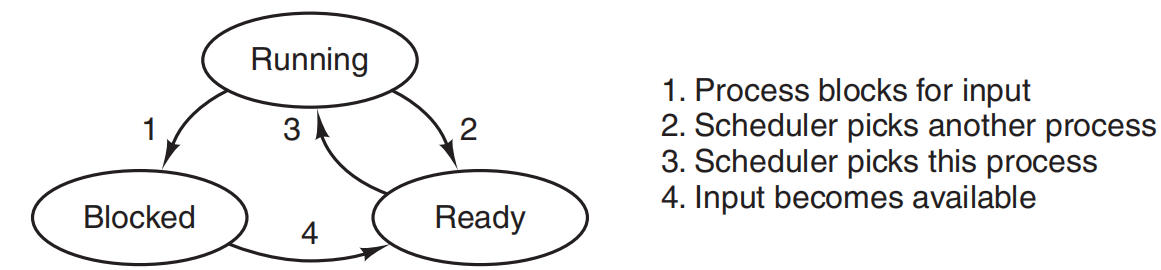
\includegraphics[width=0.85\textwidth]{FIG/2-2.png}
		\caption{一个进程有运行,就绪和阻塞三种状态,该图展示了进程如何在这三种状态下转换} \label{fig:processstatus}
	\end{figure}

	在这三种状态中,有四种转换方式。当操作系统发现一个进程不能立即继续的时候发生转换1。进程有时候可以执行一个系统调用如Pause,来进入阻塞状态。在其他的系统中,包括UNIX,当一个进程从一个管道或特殊文件中读取数据的时候,而且那时还没有可用的输入,则该线程自动进入阻塞状态。迁移3发生在所有其他进程都有了公平的份额,并且是第一个进程让CPU再次运行的时候了。调度的主题,即决定哪个进程应该运行什么时候、多长时间,是一个重要的问题;我们将在本章后面讨论它。许多算法被设计用来平衡系统的整体完全需求,以及保证对每一个进程的公平性。我们将在本书的稍后谈论到这些。迁移4发生在一个进程等待外部事件发生的时候。如果没有其他的线程在那时运行,则过程3将被触发,进程将开始运行。否则,它将需要在就绪状态进行一会等待,直到CPU可以用了才轮到它。
	使用这个进程模型,思考系统内部发生的事情变得容易得多。一些进程执行用户键入的命令程序,还有一些进程是系统的一部分,它们处理像文件服务的请求,管理运行一个磁盘或者一个磁带的具体细节。当一个磁盘中断出现的时候,系统决定停止运行现有的进程并运行磁盘进程,该进程因为之前等待中断而处于阻塞状态。因此,就可以不再考虑中断,而只是考虑用户进程,磁盘进程和终端进程等等,当他们在等待一些事情发生的时候。当磁盘被读取或者字符被键入的时候,等待它的进程已经解除阻塞,可以再次运行了。
	
	这个视图产生了图 \ref{fig:scheduler} 所示的模型。这里操作系统中最底层级的是调度器,它的上面是一系列的进程。所有的中断处理和实际运行和停止进程的细节都隐藏在调度器的里面了,调度器的实际上代码不多。操作系统的其余部分在流程形式上结构良好,然而,很少有真正的系统像这样结构良好。 

	\begin{figure}[ht]\small
		\centering
		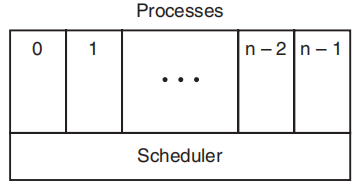
\includegraphics[width=0.85\textwidth]{FIG/2-3.png}
		\caption{最底层基于进程的操作系统处理中断和调度,在此层之上是顺序进程} \label{fig:scheduler}
	\end{figure}

	\subsection{进程实现}
	
	为了实现进程模型,操作系统维护一个表,称为进程表(一个数组结构),每一个进程有一个进程表项,一些作者称这些表项为进程控制块(PCB)。这个表项包含进程状态的重要信息,包括它的程序计数器,栈指针,内存分配地址,所打开文件的状态,它的计数与调度信息,以及进程当进程从运行态切换到就绪态和阻塞态时,必须保存的其他内容,这样它可以在稍后重新启动,就好像从未被停止过一样。
	
	图 \ref{fig:processentry} 给出了一个典型系统的关键字段,第一列中的字段关于进程管理,另外两个分别是关于内存管理和文件管理的。值得注意的是进程包含的字段是和具体的系统强关联的,各个系统可能会有很大的不同,但是该图给出了所需要信息类别的基本情况。

	\begin{figure}[ht]\small
		\centering
		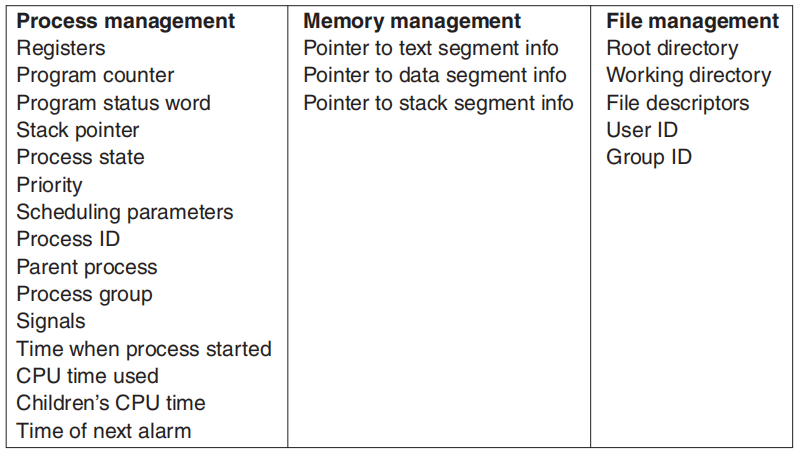
\includegraphics[width=0.85\textwidth]{FIG/2-4.png}
		\caption{一个典型的进程表项的字段} \label{fig:processentry}
	\end{figure}

	现在我们来看一下进程表,现在可以稍微多解释一些多个顺序进程是如何在一个CPU上进行管理的。和每一个I/O类别相关的是一个叫做中断向量(interrupt vector)的位置(通常位于内存底部空间的一个固定位置),它包含了中断服务过程的地址。想象一下,在用户进程3运行的时候一个磁盘中断发生了。用户进程3的程序计数器,程序状态字,有时候还有一个或多个寄存器被中断控制硬件压入到当前栈中。计算机接着就跳入到中断向量的特定地址上了,这些都是硬件所做的。从现在开始,主要就依赖软件了,特别是中断服务过程。
	所有的中断通过保存寄存器开始的,通常在当前进程的进程表条目中。接着被中断压入栈的信息被移除而且栈指针被设置指向一个暂时的栈
	进程处理器。
	像保存寄存器和保存栈指针等操作,甚至不能使用像C语言一样的高级语言进行表达,所以它们使用汇编语言的一个例程进行表达。通常对于所有的中断该例程都是可用的,因为保存寄存器的功能是可用的,不管引起中断的原因是什么。
	当这个例程结束的时候,它调用一个C过程来处理某个中断类型剩下的工作(我们假定操作系统是用C语言编写的,通常实际的操作系统都是用C语言编写的)。当完成这些工作后,一些进程可能就处于就绪状态了,调度器被调用来决定哪一个进程接下来被运行。
	中断处理和调度如图 \ref{fig:interupt} 所示。值得注意的是,细节随着系统的不同有可能会有所不同。

	\begin{figure}[ht]\small
		\centering
		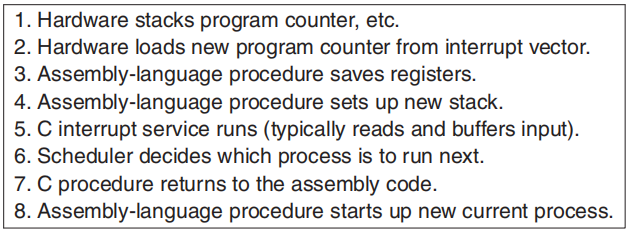
\includegraphics[width=0.85\textwidth]{FIG/2-5.png}
		\caption{中断发生后操作系统最底层的工作步骤} \label{fig:interupt}
	\end{figure}
	
	另外一个更好的模型是从概率的角度来考察CPU的利用率。假设一个进程在等待I/O完成时花费了它的一小部分时间。如果在内存中有n个进程,n个进程都在等待I/O的概率是p$^{n}$。CPU的利用率可以使用公式: \begin{center} CPU利用率 = 1 − p$^{n}$ \end{center} 表示。
	
	图 \ref{fig:multiprogrammingdegree} 给出了CPU的占用率是n的函数,我们称为多道程序设计的道数。
	
	\begin{figure}[ht]\small
		\centering
		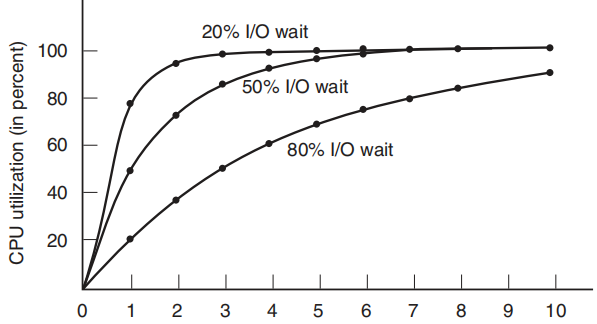
\includegraphics[width=0.85\textwidth]{FIG/2-6.png}
		\caption{CPU的利用率是内存中进程数目的函数} \label{fig:multiprogrammingdegree}
	\end{figure}

	从图中我们可以看到,进程在使用80\%的时间在等待I/O。至少有10个进程同时驻留在内存中以使得CPU的空闲率低于10\%。当您意识到等待用户在终端输入内容(或单击图标)的交互进程处于I/O等待状态时,应该很清楚,80\%或更多的I/O等待时间并不罕见。但是,即使在服务器上,执行大量磁盘I/O的进程通常也会有这个百分比或更多。
		
	为了准确起见,应该指出的是概率模型描述的只是一个估计的值。它隐式地假设所有n个进程都是独立的,这意味着内存中有五个进程的系统,其中有三个进程在运行,两个进程在等待是可以接受的。但是对于只有一个CPU,我们是不能同时运行三个进程的,因此,一个进程在CPU繁忙时准备就绪就必须等待。因此,这些过程不是独立的。可以使用队列理论建立一个更精确的模型,但是,我们所做的多道程序设计的要点是,让进程在CPU空闲时使用它,当然,仍然有效,即使的真实曲线与图中所示的曲线略有不同。尽管图 \ref{fig:multiprogrammingdegree} 所表示的模型思想简单,但是它仍然可以对CPU的性能进行特定的预测,尽管只是粗略地预测。
	假设,例如,一台计算机有8GB的内存,操作系统及其表占用2GB,每个用户程序也占用2GB。这个大小就允许有三个用户程序同时在内存中。对于平均80\%的I/O等待,我们有CPU的平均利用率(忽略操作系统的开销)为 1-0.8$^{3}$ 49\%。再增加8GB的内存可以使得系统从3道多道程序编程到7道多道程序编程,因此可以将CPU的利用率提升至79\%。换句话说,额外增加8GB内存可以使得吞吐率提升30\%。
	当然,再增加8GB内存只能使得CPU的利用率从79\%增加到91\%,仅仅只是增加了12\%的吞吐率。使用这个模型,计算机的拥有者可以判断出来,第一次增加内存的投资是划算的,而第二次增加内存的投资就不那么值得了。
	
	\section{线程}
	
	在传统的操作系统中,每一个进程都有一个地址空间和一个单个的控制线程。事实上,这几乎是进程的定义。不管怎么说,在很多的情况下,总是希望多个控制线程在同样的地址空间并以准并行化的方式处理,就好像他们是独立的进程一样(除了共享地址空间)。在接下来的章节中我们将这些情况和他们的影响。
	
	\subsection{线程的使用}
	
	为什么人们在进程内部还要有一个进程? 有若干理由说明产生这些迷你进程(线程)的重要性。现在让我们探讨一下其中的一些原因。有线程的主要原因是在许多的应用程序中,会同时发生多种活动,一些可能随着时间的推移被阻塞。通过将这些应用程序分解成多个可以准并行运行的顺序线程,可以使程序设计模型变得简单。
	
	前面已经进行了有关的讨论。准确地说,这正是之前关于进程模型的讨论。除了考虑中断,定时器和上下文切换,我们还可以考虑并行进程。
	只是现在对于线程我们增加了一个新的元素:并行的实体共享一个地址空间,并且在它们之间共享数据。这个能力对于一些应用程序而言非常地关键,而这正是多进程模型(它们具有不同的地址空间)所无法表达的。
	
	第二个需要多线程的理由是,因为线程比进程更加轻量级,它们比进程更加容易被创建和销毁。在许多系统中,创建一个线程通常比创建一个进程要快10-100倍。当线程的数量需要动态和快速地变化时,这个性质就非常地有用。
	
	使用线程的第三个原因涉及性能方面的考量。当所有线程都是CPU密集型的是时候,它们不会产生性能提升,但是如果线程既有顺序计算又有顺序I/O的时候,线程允许这些活动的重叠,从而可以提升这些应用程序的性能。
	
	做后,线程在拥有多个CPU的系统上是很有用的,因为可以实现真正的并行。我们将在第8章回过头来讨论这个问题。
	
	通过查看一些具体的示例,可以很容易地看出线程为什么有用。我们先考虑第一个例子,一个文字处理软件。文字处理程序通常在屏幕上显示正在创建的文档,因为它在屏幕上精确地显示文档。特别地,所有的换行和换页都在他们正确和最终的位置上。以便用户可以检查它们,并在需要时更改文档(比如,消除孤行,在一页上的不完整的底部行或者顶部行,因为它们看起来不够美观。)
	设想用户正在写一本书,从作者的角度看,把一本书的作为一个单独的文档,进行全书查找和全局替换的时候是最方便的。另一种方法是,每一章作为一个独立的文件。但是,把每一节和每一小节作为一个独立的文件,在进行全局替换的时候就会变得非常麻烦,因为它们可能要对上百个文件逐一进行编辑。例如,如果"某某标准草案"在书籍出版发行之前被批准了,则必须将"某某标准草案"改为"某某标准"。如果整本书只有一个文件,那么只要对一个文件进行替换处理就可以了,但是如果整本书被分成了几百个文件,则就要一个一个地对其进行修改。
	
	现在考虑,如果现在用户在一个有800页的书籍的第一页上删除一个语句,会发生什么情形。在检查了所修改的页面并确认正确以后,他想在第600页再做一次修改,并且键入一个命令告诉文字处理程序跳转到第600页(可能要查阅只是出现在那里的一个短语)。于是,字处理软件就需要对整本书的前600页进行重新排版,因为在它重新处理完前600页之前,它不知道第600页现在第一行的内容是什么。而在第600页的页面真正在屏幕上显示出来之前,计算机可能需要出现一定的延迟,这将导致用户的体验变差。
	
	多线程可以在这个时候发挥作用。想象一下文字处理软件被写成了一个两个线程的程序。一个线程用于前台和用户交互,另一个线程在后台处理重新排版。一旦第一页的一句被删除掉,交互线程立即通知排版线程立即对全书进行重新地排版。于此同时,交互线程继续监听键盘和鼠标,并响应一些简单的用户操作,如滚动页面1,而另一个线程在正后台疯狂地执行运算。幸运的是,重现排版可以在用户要求跳转到第600页之前完成,这样就可以直接显示第600页给用户了。
	
	既然做到了这个地步,那为什么不增加第三个线程呢。很多的文字处理软件都有每隔几分钟自动地保存真个文件到磁盘上的功能,防止用户在程序崩溃,系统崩溃和断电的情况下丢失掉一整天的工作。第三个线程就可以处理磁盘备份,而不对另外两个线程产生干扰。图 \ref{fig:multithreads} 给出了有三个线程的情形。

	\begin{figure}[ht]\small
		\centering
		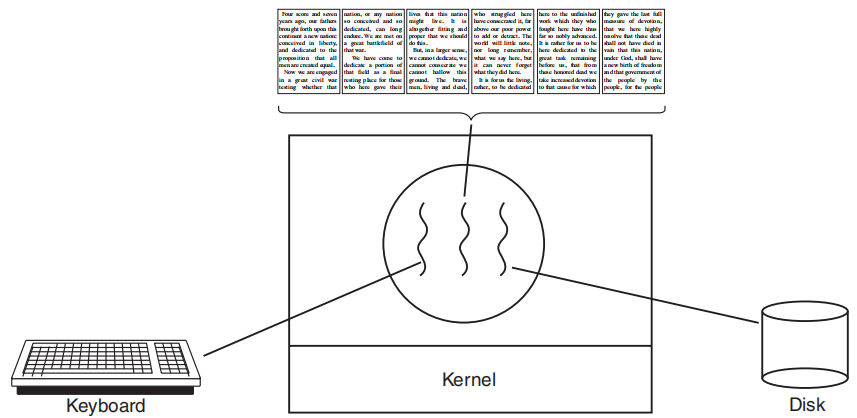
\includegraphics[width=0.85\textwidth]{FIG/2-7.png}
		\caption{一个拥有三个线程的文字处理软件} \label{fig:multithreads}
	\end{figure}
	
	如果一个程序是单线程的,那么不管什么时候开始进行磁盘备份,来自键盘和鼠标的命令在备份完成之前都将被忽视。用户当然会认为这样性能是很差的。另外,键盘和鼠标事件可以中断磁盘备份,可以实现好的性能,但是将会导致一个复杂的中断驱动编程模型。有了三个线程,编程模型就变得简单多了。第一个线程和用户进行交互,第二个线程对文档进行处理,第三个线程负责定时将RAM中的内存往磁盘备份。
	
	很清楚的是,如果有三个进程则不会这样,因为三个线程都需要操作文档。通过三个线程而不是三个进程,线程间可以共享同一块内存,因此都可以访问正在被编辑的文档,而三个进程则不可能做到这样。
	
	许多交互式程序都有类似的情形。例如,一个电子的表格允许用户维护一个矩阵,它的一些元素是用户提供的数据,另外一些元素是基于用户输入的数据采用可能比较复杂的公式计算出来的数据。当用户更改一个元素时,可能需要重新计算很多其他的元素。有一个后台线程进行这些计算,交互线程可以让用户在后台执行计算的时候进行额外的改变。类似地,第三个线程可以定期地执行磁盘备份。
	
	现在考虑线程有用的另外一个例子:一个网站的服务器。对于页面的请求进入,同时被请求的页面返回给客户端。在大多数的网站中,有一些网页的访问频率远远高于其他网页。例如,Sony主页的访问频率要远远高于深藏在页面树里的任何一款照相机的技术说明网页。网络服务器利用这个事实来将一些经常被访问的网页放到内存中,消除了需要去磁盘上取出它们的必要。像这样的集合被称为缓存,也在许多其他的场景中得到应用。我们已经在第一章中讨论了CPU的缓存。
	
	一种组织网络服务器的方式如图 \ref{fig:multithreadswebserver} 所示。这里有一个派发器线程,读取来自网络的请求。在检查完请求后,它选择一个空闲的工作线程来处理这个请求,可能是通过将一个指向消息的指针写入与每一个线程特定的字里。分派器唤醒睡眠工作线程,并将它从阻塞状态移到就绪状态。
	
	\begin{figure}[ht]\small
		\centering
		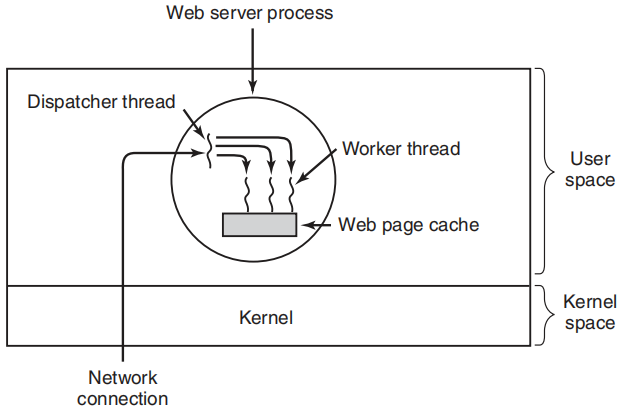
\includegraphics[width=0.85\textwidth]{FIG/2-8.png}
		\caption{一个多线程的网络服务器} \label{fig:multithreadswebserver}
	\end{figure}

	当工作进程唤醒的时候,它检查该网页请求可以从所有线程都可以访问的网页缓存中找到。如果不能找到,则开始一个\texttt{read}操作,从磁盘中读取该网页,并且阻塞该线程直到磁盘操作结束。
	
	当线程在磁盘操作上阻塞的时候,另外一个线程将被选择运行,可能是分派器,以获取更多的工作,或者是另外一个已经就绪的工作线程。
	
	这个模型使得服务器可以被写成一组顺序线程。分派器程序包括一个无限循环以获得工作请求,并把它交给工作线程。每一个工作线程的代码都有一个无限循环来接收来自分派器的请求和检查所请求的网页是否在网页缓存中。如果在,就把它返回给客户端,然后工作线程阻塞直到新的请求到来。如果不在,则从磁盘中获取该网页,并返回给客户端,接着阻塞等待一个新的请求。
	
	图 \ref{fig:coderouting} 给出了有关代码的大致框架。在这里,还有本书剩余的部分,\texttt{TRUE}被设定为常量1。同样,\texttt{buf}和\texttt{page}分别保存工作请求和网页的相应结构。
	
	\begin{figure}[ht]\small
		\centering
		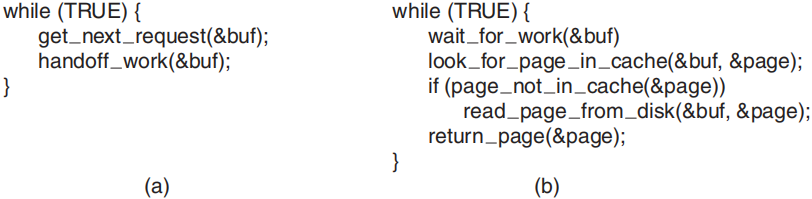
\includegraphics[width=0.85\textwidth]{FIG/2-9.png}
		\caption{图2-8的代码架构 (a)分派器线程 (b)工作线程} \label{fig:coderouting}
	\end{figure}
	
	考虑一下没有线程网页服务器该如何实现。一种可能是让他作为一种可以操作的单个线程。网页服务器使用一个主循环获得请求,检查它,并在下一个请求到来之前把它执行完毕。当等待磁盘的时候,服务器是空闲的并且不处理其他任何到来的请求。如果网页服务器运行在一个特定的机器上,而且这是通常的情况,当网页服务器在等待磁盘的时候CPU就是简单的空闲。结果就是每秒只有很少的线程被处理,所以,线程很好地改善了性能,而且每个线程通常是按照顺序编程的。
	
	目前为止,我们看到了两种可能的设计:一个多线程的网络服务器和一个单线程的网络服务器。假设一下多线程如果不可行,而系统设计者发现由于单线程带来的性能损失是不可以接受的。如果一个不阻塞的\texttt{read}系统调用是可用的,则还可以有第三种方法。当一个请求来的时候,唯一的线程就会检测到它。如果它可以从缓存中得到满足,则很好,如果不能,一个非阻塞的磁盘操作就开始了。
	
	服务器在一个表格中记录下当前请求的状态,接着去取下一个事件。下一个事件可能是一个新工作的请求也可能是前一个操作从磁盘返回的回应。如果是新的工作,则开始工作。如果是从磁盘返回的回复,将会从表格返回相关的信息,并处理回复。对于不阻塞的磁盘I/O,回复可能需要以信号或者中断的形式返回。
	
	在这个设计中,我们在头两个模型中的“顺序进程”模型消失了。计算的状态每次都必须显式地保存在表中,当服务器从一个请求切换到另外一个请求的时候。事实上,我们在以一种非常硬核的方式模拟线程和它的栈。一种像这样的设计,在其中每一个计算都有保存的状态,而且存在一些事件可以出现来改变这种状态,被称为“有限状态机”。这个概念在计算机科学中被广泛地应用着。
	
	现在对于线程应该提供什么就已经非常清楚了。它们使我们能够保留顺序进程的思想,即进行阻塞调用(例如,对于磁盘I/O),并且仍然能够实现并行性。阻塞系统调用可以使得编程变得简单,而且并行性可以改善性能。单线程的服务器保持了阻塞系统调用的简单性但是放弃了性能。第三种方法通过并行性取得了高的性能但是使用了非阻塞的调用和中断,因而很难编程。这些模型的优缺点都在图 \ref{fig:threeways} 中所示了出来。
	
	\begin{figure}[ht]\small
		\centering
		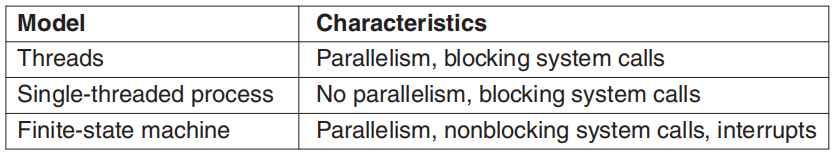
\includegraphics[width=0.85\textwidth]{FIG/2-10.png}
		\caption{构建服务器的三种方式} \label{fig:threeways}
	\end{figure}
	
	第三个关于进程作用的例子是那些必须处理极大数量数据的应用。通常的方式是读入一个数据块,处理它,并把它写出。这里的问题是如果仅仅只能用阻塞的系统调用,进程在数据输入或输出的时候就会被阻塞。在需要有大量的计算的时候,使得CPU空闲,无疑是浪费的,应该尽量避免。
	
	多线程提供了一种解决方案。进程可以被分解成一个输入线程,一个处理线程和一个输出线程。输入线程读入数据到一个缓冲区中,处理线程从缓冲区中取出数据,处理它们,并把结果放置到一个输出缓冲区中。输出缓冲区将这些结果写回到磁盘。在这种方式下,输入,输出和处理可以同时进行。当然,这个模型仅仅在系统调用只阻塞调用线程的时候才有用,而不是阻塞整个进程。
	
	\subsection{经典的线程模型}
	
	现在我们已经看到为什么线程是有用的而且它是如何被使用的,让我们更多地调查一下这个想法。进程模型基于两个基本的概念:资源分组和执行。有时候很难去区分它们,这就引入了线程的概念。首先,我们看一下经典的线程模型,接着我们将看一下Linux的进程模型,它模糊了进程与线程的分界线。
	
	理解进程的一个视角是,它是一个组织相关资源在一起的方式。一个进程有一个包含程序文本和数据的地址空间,同样也有其他的资源。这些资源可能包括打开的文件,子进程,即将发生的定时器,信号处理程序,账户信息等等。把它们以进程的形式放在一起,可以更好地进行管理。
	
	进程的另外一个概念是一个正在运行的线程,通常被简称为线程。这个线程有一个程序计数器来跟踪接下来执行哪一条指令。它有寄存器,来保存现有的工作变量。它有一个栈,来包含执行历史,每一个过程都有一帧,但是尚未返回的帧。尽管一个线程必须在一些进程中执行,线程和进程是不同的概念,可以分别给予处理。进程可以被用来组织资源,线程是在CPU上被调度的执行实体。
	
	线程给进程模型带来的丰富是允许多个执行操作在一个相同的进程环境中发生,允许彼此之间有较大独立性的多个线程执行。在一个进程有多个线程并行执行类似于在一台计算机中有多个进程并行执行。在前一个情况下,线程之间共享地址空间和其他的资源,在第二种情况下,进程共享物理内存,磁盘,打印机和其他资源。因为线程有一些进程的性质,它们有时候又被称为轻量级线程。术语"多线程"也被用来描述在一个进程中有多个线程的情况。就像我们在第一章中看到的那样,一些CPU有一些对多线程的直接硬件支持,并且允许线程在纳秒级时间内进行切换。
	
	在图 \ref{fig:processthread} (a)中我们看到三个传统的进程。每一个进程都有它的地址空间和单个控制线程。相反,在图 \ref{fig:processthread} (b)中我们看到一个进程有三个控制线程。尽管两种情况下我们都有三个线程,在图 \ref{fig:processthread} (a)每一个进程都操作在一个不同的地址空间上,而在图 \ref{fig:processthread} (b)中三个进程共享同一个地址空间。
	
	\begin{figure}[ht]\small
		\centering
		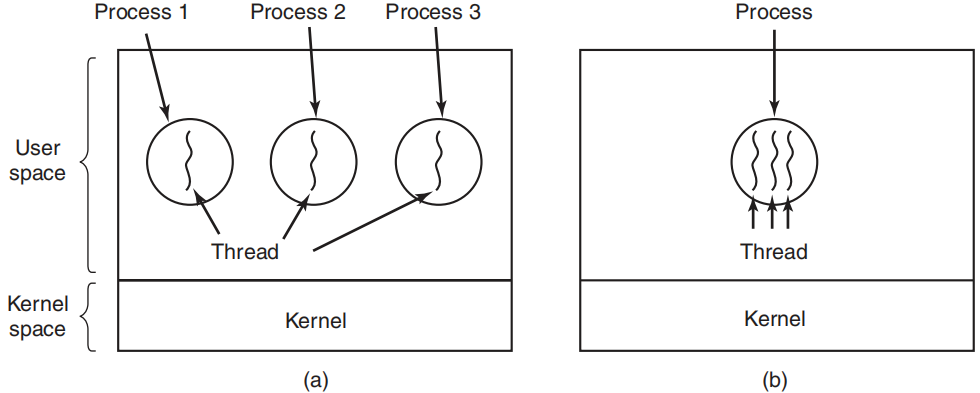
\includegraphics[width=0.85\textwidth]{FIG/2-11.png}
		\caption{a)三个进程每个含有一个线程,b)一个进程包含三个线程。} \label{fig:processthread}
	\end{figure}

	当一个多线程的进程运行在一个单CPU的系统上时,线程轮流被执行。图 \ref{fig:processconcept} 给出了一个多道编程的进程是如何工作的。通过在多个进程之间来回地切换,系统给出了多个顺序进程是并行执行的假象,多线程也是这样工作的。CPU在多个线程之间来回地切换,提供了多个线程也是并行执行的假象,好像它们运行在比实际CPU更慢一些的CPU上。在一个有三个计算密集型的线程的进程中,线程可以表现出并行的性质,每一个线程得到真实CPU速度的三分之一。
	
	一个进程中的不同线程不像不同的进程那样地相互独立性。所有的线程都有相同的地址空间,同时也意味着它们共享相同的全局变量。因为每个线程都可以访问进程地址空间的每一个内存地址,一个线程可以读,写甚至清空另一个线程的栈。线程之间没有保护,因为: 1)不可能, 2)也不必要。和不同的进程不同,可能来自不同的用户,而且彼此之间可能还有敌意,一个进程总是被单个用户所拥有,它们大概总会创建多个线程,线程之间是相互合作而不是斗争。除了共享地址空间,所有的线程还可以共享打开的文件集,子进程,时钟,信号等等。像图 \ref{fig:sharecontents} 所示的那样。

	\begin{figure}[ht]\small
		\centering
		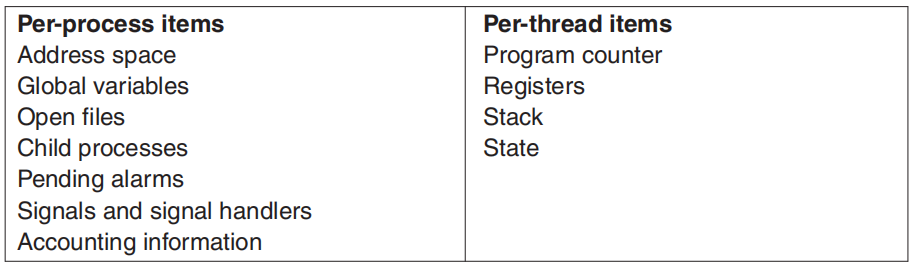
\includegraphics[width=0.85\textwidth]{FIG/2-12.png}
		\caption{a)第一列给出了线程间共享内容 b)第二列给出了线程间私有内容} \label{fig:sharecontents}
	\end{figure}
	
	第一列中的项目是进程属性,不是线程属性。例如,如果一个线程打开了文件,这个文件对于进程中的其他线程也是可见的,它们可以进行读和写。这是合理的,因为进程是进行资源管理的单元,不是线程。如果每一个线程都有它的地址空间,打开的文件,挂起的时钟等等,它将会是一个独立的进程。我们努力通过线程的概念来使得多个线程可以执行来获取一组资源这样它们就可以一起紧密地合作来完成工作任务。
	
	像一个传统的进程(一个进程仅仅只有一个线程),一个线程只能是以下几种状态的一种:运行,阻塞,就绪或终止。一个运行的线程当下拥有CPU并且是活动的。相比较而言,一个阻塞的线程等待一些将它解除阻塞的事件发生。例如,当一个线程执行一个系统调用从键盘读取数据的时候,该线程就被阻塞直到输入被键入。一个线程可以处于阻塞状态直到一些外部的事件发生,或者等待其他的线程来解阻塞它。一个就绪的线程将被安排运行,而且一到轮到他就会被运行。线程之间的状态转换和进程之间的状态转换是一样的,如图 \ref{fig:processstatus} 所示。
	
	意识到每一个进程都有自己的堆栈是非常重要的,像图 \ref{fig:threadstack} 中所示的那样。每个线程的堆栈包含一个帧,用于调用的每个过程但是尚未从返回。
	
	\begin{figure}[ht]\small
		\centering
		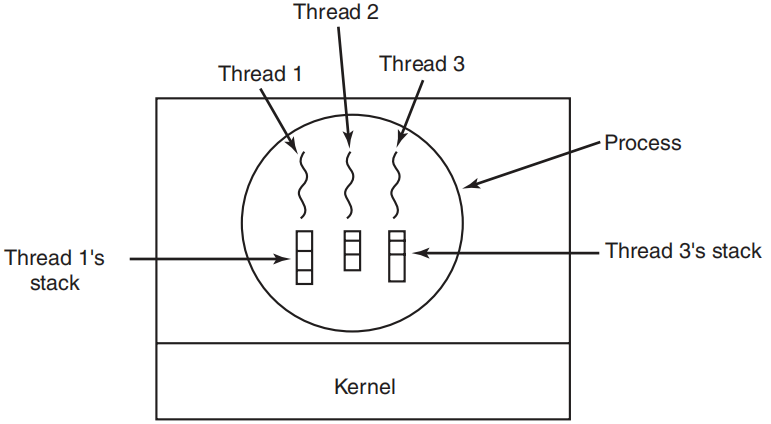
\includegraphics[width=0.85\textwidth]{FIG/2-13.png}
		\caption{每一个线程都有自己的栈} \label{fig:threadstack}
	\end{figure}

	这个帧包含过程的局部变量和过程调用结束后的返回地址。例如,如果过程X调用过程Y,过程Y调用过程Z,而过程Z正在被执行。则过程X,Y和Z的帧都将在栈上。每一个线程都会调用不同的过程并且都有一个不同的执行历史。这就是为什么每一个线程需要它自己的栈的原因。
	
	当多线程存在的时候,进程可能会从一个单线程开始。线程拥有创建新线程的能力通过调用库过程,如\texttt{thread\_create}。
	一个\texttt{thread\_create}的参数指定新线程运行过程的名字。没有必要指定新线程的地址空间,因为新线程会在创建线程的地址空间中自动运行。一些线程是有层次的,有父子关系,但是这种关系并不常见,大部分情况下线程之间是平等的。无论有没有层次关系,创建的线程都会返回一个标识符,该标识符也就是新线程的名字。
	
	当一个线程终止了它的工作,它可以通过调用一个库过程退出,称为\texttt{thread\_exit},接着它就消失了并且不会被调度了。在一些线程系统中,一个线程可以通过调用一个过程来等待另外一个线程退出,例如\texttt{thread\_join}。这个过程阻塞调用它的线程直到另一个线程退出。在这一点上,线程的创建和终止非常类似于进程的创建和终止,也有大致相同的选择。
	
	另外一个常见的线程调用是\texttt{thread\_yield},允许一个线程主动地放弃CPU并让另外一个线程运行。这样的调用很重要,因为没有时钟中断可以像进程那样实际执行多道程序设计。因此,线程非常友善地主动放弃CPU让其他线程运行是非常重要的。有的调用允许一个线程等待另一个线程完成它的工作,或让一个线程宣称它已经完成了一些工作,等等。
	
	虽然线程很有用,但是它们也同时给编程模型带来了许多其他的复杂性。一开始,考虑一下UNIX中的系统调用。如果父进程中有多个线程,那么子进程中是不是也应该有多个线程呢? 如果不是,则进程可能不能正常地工作,因为在该子进程中的线程都是绝对必要的。
	
	然而,如果一个子进程像父进程一样拥有同样多的线程,如果父线程在读调用(例如,从键盘)被阻止,会发生什么情况? 那是不是两个线程被阻塞到键盘上了,一个是父进程,一个是子进程? 当键入一行命令的时候,是不是两个线程同时获得了相应的副本? 还是仅仅是父进程,仅仅是子进程。
	
	另外一类问题是关乎线程共享许多数据结构的事实。当一个线程关闭一个文件而另一个线程还在读取它的时候会发生什么。假设一个线程发现内存太少而开始分配更多的内存。在工作一半的时候,发生了进程切换,新的线程同时也注意到了内存太少并开始分配更多的内存。内存有可能被分配两次,这个问题可以通过一些努力给解决,但是需要仔细的思考和设计才能使多线程程序能够正确地工作。
	
	\subsection{POSIX进程}
	
	为了实现可移植的线程程序,IEEE制定了一个关于线程的标准: IEEE 1003.1c。它定义的线程包被称为Pthreads。大部分UNIX的系统支持它。这个标准定义了超过60个函数调用,太多了不能一一列举。这里我们只列举几个主要的来说明它是怎么工作的。
		
	\begin{figure}[ht]\small
		\centering
		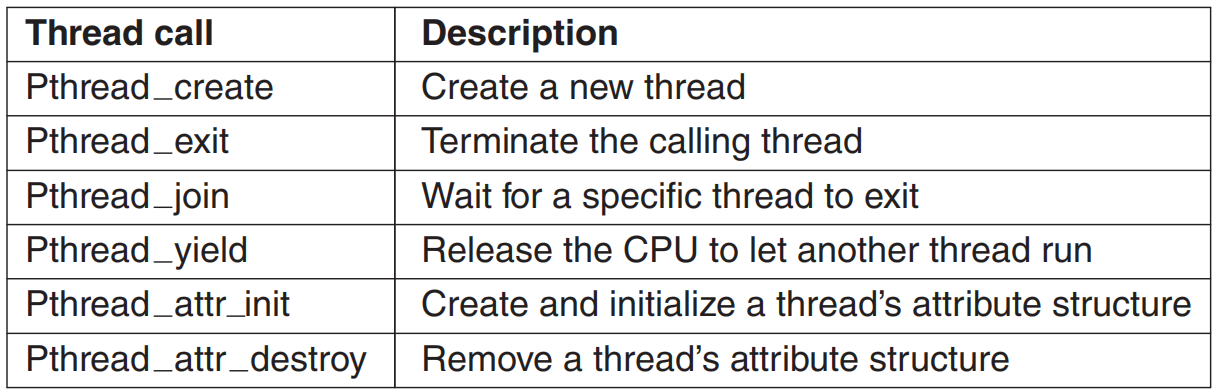
\includegraphics[width=0.85\textwidth]{FIG/2-14.png}
		\caption{一些Pthread函数调用} \label{fig:pthread}
	\end{figure}

	所有的Pthreads线程都有特定的性质。每一个都有一个标识符,一组寄存器(包括程序计数器)和一组属性,被存储在一个结构中。这些属性包括栈大小,调度参数,还有一些其他使用线程所需要的项目。
	
	一个新线程的创建使用\texttt{pthread\_create}调用。新创建线程的线程标识符作为函数返回值使用。这个调用非常类似与fork系统调用(除了参数),线程标识符扮演着PID的角色,主要用于识别其他调用中引用的线程。
	
	当一个线程已经完成了分配给它的工作,它可以调用\texttt{pthread\_exit}终止。这个调用中止线程并释放它的栈。
	
	一般一个线程在继续需要等待另外一个线程完成它的工作并退出。等待的线程调用\texttt{pthread\_join}来等待另一个特定的线程终止。被等待线程的线程标识符被当作参数传递。有些时候碰巧有些线程逻辑上没有被阻塞,但是感觉它已经运行了很长的时间,并且想给另外一个线程运行的机会。它可以通过\texttt{pthread\_yield}系统调用来实现。对于进程则没有这样的假设,因为我们假设进程之间是激烈竞争的,每一个进程都想获得所有的CPU时间。然而,因为一个进程中的所有的线程都是在一起工作的,它们的代码也大部分是一个人写的,有时候编程者希望这些线程互相能给对方一个机会。
	
	接下来的两个系统调用,处理属性。\texttt{Pthread\_attr\_init}创建和一个线程相关的属性结构,并把它们初始化为默认值。这些值(如优先级)可以通过操作属性结构中的字段来进行改变。
	
	最后,\texttt{Pthread\_attr\_destory}移除一个进程的属性结构,释放它的内存。它不会影响调用它的线程,调用它的线程会继续存在。
	
	为了更好地体验Pthreads是如何工作的,考虑一下图 \ref{fig:threadexample} 所示的简单例子。
	
	\begin{figure}[ht]\small
		\centering
		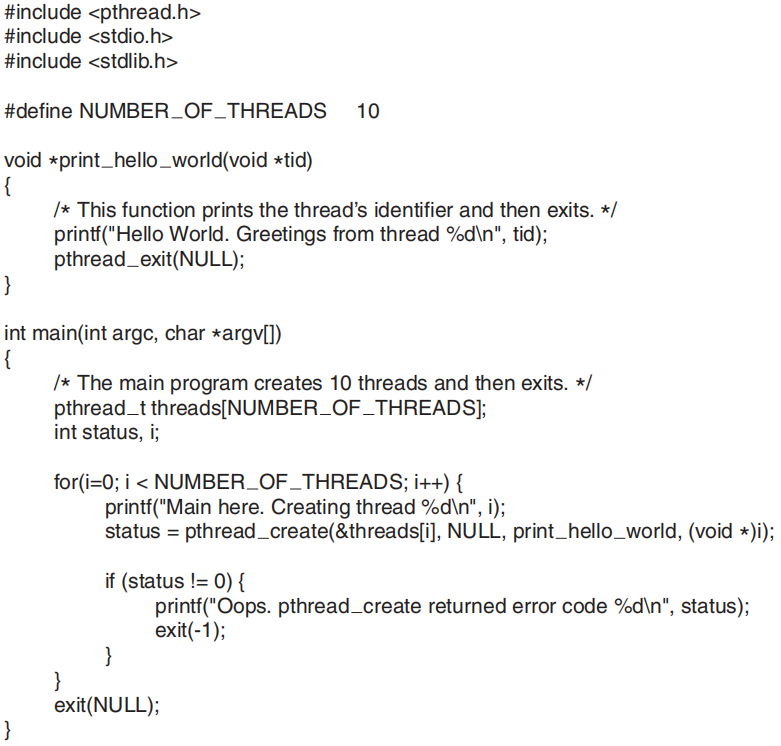
\includegraphics[width=0.85\textwidth]{FIG/2-15.png}
		\caption{一个使用线程的示例程序} \label{fig:threadexample}
	\end{figure}
	
	这里主程序循环了\texttt{NUMBER\_OF\_THREADS}次,在每一次的迭代中创建一个新的线程,在声称了它的打算之后。如果线程创建失败了,它打印一个错误信息并退出。在创建了所有的线程后,主程序退出。
	
	当一个线程被创建后,它打印一个一行的程序来声称它自己,接着就退出。各种信息交织的顺序是不确定的,在程序运行时可能会有所不同。
	以上谈论的Pthread调用不是全部的,我们将看一下其他的系统调用在讲述完进程和线程同步后。
	
	\subsection{在用户空间实现线程}
	
	有两个主要的地方用来实现线程:用户态和内核态。这两者之间的选择稍微有些争议,有时候混合的方案也是可能的。我们将描述这些方法,以及它们0的优点和缺点。
	
	第一种方法是将整个的线程包放到用户空间中。内核不知道它的任何内容。内核关心的,是管理单线程的普通进程。首先,也是最明显的,一个用户级别线程包的好处是它可以实现在一个不支持多线程的操作系统之上。所有的操作系统都曾经属于这一类,甚至直到现在还有一些操作系统是这样的。通过这种方法,操作系统被实现成一个库。
	
	所有的这类实现都有相同的通用结构,如图 \ref{fig:threadpackage} 所示。
	
	\begin{figure}[ht]\small
		\centering
		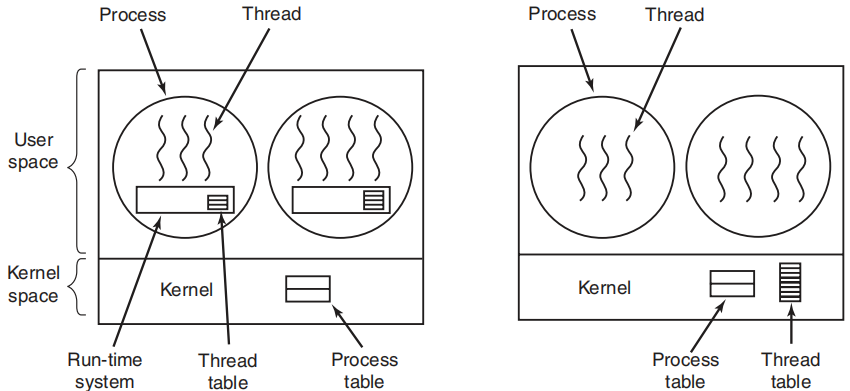
\includegraphics[width=0.85\textwidth]{FIG/2-16.png}
		\caption{(a) 一个用户级线程包 (b) 一个被内核管理的线程包} \label{fig:threadpackage}
	\end{figure}

	线程运行在运行时系统之上,运行时系统是管理线程的过程的集合。我们已经看过了四个调用: \texttt{pthread\_create}, \texttt{pthread\_exit}, \texttt{pthread\_join},和\texttt{pthread\_yield},但是通常还有更多。
	
	当线程在用户态进行管理的时候,每一个进程都需要有它私有的进程表来跟踪在进程内的线程。这个表格和内核中的进程表类似,但它只跟踪每个线程的属性,例如每个线程的程序计数器、堆栈指针、寄存器、状态等等。线程表是被运行时系统管理的。当一个线程被移至就绪态或者阻塞态,它将重启需要的信息存放到进程表格中,就像内核将进程状态存放到进程表格中是一样的。
	
	当线程做了一些可能导致它本地阻塞的操作,例如,等待线程里面的另一个线程来完成工作,它调用一个运行时过程。此过程检查线程是否必须置于阻塞状态。如果是,它存储线程的计数器(线程本身的)在线程表格中,在表中查找就绪的线程运行,并且将线程保存的值重新载入机器的寄存器中。只要线程的栈指针和程序计数器切换好,新的线程就会自动地被重新执行。如果机器正好有一个指令存储所有的寄存器以及另外一条指令把他们进行加载,则整个线程切换可以在数条指令内完成。这样进行线程切换只有比陷入内核执行切换要快一个数量级,这是使用用户级线程包一个极大的优点。
	
	但是,还有一点和进程有很大的不同。当一个线程在某一个时刻停止运行的时候,例如,它调用了\texttt{thread\_yield},\texttt{thread\_yield}的源代码可以在线程表中保存线程自身的信息。另外,它可以调用线程调度器来选择另外一个要运行的线程。保存线程状态和调度的过程都是本地过程,所以触发它们比执行一个内核系统调用要方便地多。另一方面,不需要陷入内核,不需要上下文切换,不需要刷新内存缓存等等。这些使得线程调度非常快速。
	
	用户级线程还有一些其他的优点。它们允许每一个线程都有它们自己的线程调度算法。对于一些应用程序,例如,哪些有垃圾回收器的线程,不必担心线程在一个不方便的时刻停下来是一个加分项。它们还可以扩展地更多,因为内核线程需要在内核中有一些固定的表格空间和堆栈空间,在有很多线程的时候可能会称为一个问题。
	
	尽管用户级线程包有着更好的性能,但是也有一些主要的问题。其中首要的问题是如何实现阻塞的系统调用。假设一个线程在键盘上的键被键入之前读取键盘。让这个线程真正地执行系统调用是不可接受的,因为这将阻塞其他所有的线程。使用线程的首要目标是允许每一个线程使用正在阻塞的调用,并且阻止一个阻塞线程影响到其他的线程。对于正在阻塞的系统调用,有了阻塞系统调用,这个目标不是轻易能够实现的。
	
	系统调用可以改为非阻塞的(例如,如果没有被缓冲的字符,对键盘的read操作可以只返回0字节),但是需要修改操作系统,这个方法是不具有吸引力的。除此之外,用户级线程的一个论据是它们可以执行在现有的操作系统之上。另外,修改\texttt{read}的语义需要对许多用户程序进行修改。
	
	在这个过程中,还有一种可能的替代方案,就是如果某个调用会阻塞,就提前通知。在大多数UNIX的版本中,有一个系统调用\texttt{select}可以允许调用者通知预期的\texttt{read}是否会阻塞。当出现此调用时,库过程read可以替换为一个新过程,该过程首先执行select调用,然后在安全的情况下才执行read调用(即不会阻塞)。如果\texttt{read}调用被阻塞,有关调用就不进行,代之以运行另外一个线程。到了下次有关的运行时系统获得了控制权,就再次检查运行\texttt{read}系统调用是否安全。这个过程要求重写系统调用库的一部分,效率不高也不够优雅,但是其他的选择不多。在系统调用周围从事检查的这些代码称为包装器(Jacket或者Wrapper)。
	
	与阻塞系统调用问题有点类似的是缺页中断问题。我们将在第三章中学到这个内容。此时可以认为,把计算机设置成这样的一种工作方式,如果程序调用或跳转到不在内存中的指令,则发生页错误,操作系统将从磁盘上获取丢失的指令及其相邻指令,这就称为一个缺页中断。这个进程被阻塞当必要的指令被定位和读入的时候。如果一个线程导致了一个缺页中断,则内核甚至在没有感知到线程存在的情况下,自然地阻塞整个进程直到磁盘I/O结束的时候,尽管其他的线程是可以运行的。
	
	用户级线程包的另外一个问题是,如果一个线程开始运行,其他的线程将不会被运行除非正在运行的线程主动放弃CPU。对于一个单进程而言,没有时钟中断,使得按照轮转法进行进程轮转的方法变得不可行(轮流执行)。除非某一个线程按照自己的意志进入运行时系统,否则调度器将永远不会有机会。
	
	解决线程永远运行的问题的一个可能的解决方案是运行时系统每秒请求一次时钟信号(中断)来控制它,但这对程序来说也是粗糙和混乱的。
	不可能总是发生高频率的周期性的时钟中断,即使可能,总的开销也是非常高昂的。更多的是,线程可能也需要一个时钟中断,这样就会扰乱运行时系统使用的时钟。
	
	另外,也许是对用户级线程最大的争论性意见是,程序员通常在经常发生线程阻塞的应用中才希望使用多线程。例如,在多线程Web服务器中,这些线程持续地进行系统调用,而一旦发生内核陷阱并执行系统调用,如果旧的线程被阻塞了,那么内核就不需要再做更多的工作来切换线程了,而且让内核这样做就不需要不断地进行select系统调用来检查read系统调用是否安全。对于基本上完全受CPU限制且很少阻塞的应用程序,拥有线程有什么意义? 由于这样做没有什么益处,因此没有人会用多线程来进行计算头n个素数或者下象棋之类的工作。
	
	\subsection{在内核中实现线程}
	
	现在让我们看一下内核是如何管理和实现线程的。如图 \ref{fig:threadpackage} (b)所示,此时就不再需要运行时系统了。同时,每一个进程中也没有线程表了,相反,内核中有一个追踪系统中所有线程的线程表。当一个线程想创建一个新的线程和销毁一个现有的线程,它执行一个内核系统调用,这个系统调用通过更新内核线程表来完成线程的创建和撤销工作。内核线程表持有每一个线程的寄存器,状态以及其他的信息。同时,内核还维护传统的进程表来追踪进程。所有的可以阻塞线程的调用都被实现为系统调用,一般比运行时过程有更高的代价。当一个线程阻塞的时候,内核根据其选择,可以运行该进程中的另外一个线程(如果有就绪线程)或者其他进程中的线程。对于用户级线程,运行时系统保持运行自己进程中的线程直到内核将CPU从该进程移走(或者没有就绪进程了)。
	由于内核创建和回收线程的代价相对较大,一些系统采用一种环保的方式回收其线程。当一个线程被销毁的时候,它被标记为不可以运行状态,但是它的内核中的数据结构并不受到影响。稍后,当一个线程必须被创建的时候,旧的线程重新被激活,从而节省一些开销。线程回收同样适用于用户级线程,但是由于用户级线程的管理代价要小的多,并没有很强烈的需求去这样做。
	
	内核线程并不需要任何新的,非阻塞的系统调用。另外,如果一个进程中的线程导致了一个缺页中断,内核可以很轻易地检查该进程是否还有其他可以运行的线程,如果有,则在等待从磁盘取回该页的时候运行它们其中的一个。它们的主要缺点是系统调用的代价比较大,所以如果线程的操作(创建,终止等)比较多,就会带来很大的开销。
	
	虽然内核线程可以解决一些问题,但是它不能解决所有的问题。例如,当一个多进程的线程被复制会发生什么?新的进程是不是和父进程拥有同样多的线程,还是只有一个?在大多数情况下,最好的选择取决于新的进程接下来要干什么。如果它想调用\texttt{exec}来启动一个新的程序,可能只有一个进程是正确的选择,但是如果它想继续执行,则复制所有的进程是最佳的选择。
	
	另外一个因素是信号。要记得信号是发送给进程的,而不是线程,至少在经典模式中是这样。当一个信号到来的时候,哪一个线程应该处理它?可能线程会注册它们对哪些信号感兴趣,所以当一个信号到来的时候应该交给声称对它感兴趣的线程进行处理。但是如果两个或更多的线程都注册对某一个信号感兴趣了怎么办?这仅仅是线程引发的两个问题,还有其他更多的问题。
	
	\subsection{混合实现}
	
	很多种不同的方法都被尝试用来综合用户级线程和内核级线程的优势。一种方法是使用内核级线程,然后在它们中的一些或全部复用用户级线程,像图 \ref{fig:multiplexthreads} 所示的那样。
	
	\begin{figure}[ht]\small
		\centering
		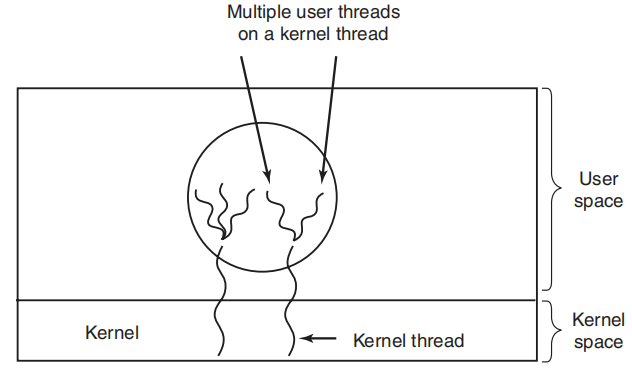
\includegraphics[width=0.85\textwidth]{FIG/2-17.png}
		\caption{将用户级线程多路复用到内核级线程} \label{fig:multiplexthreads}
	\end{figure}
	
	当采用这种方法的时候,内核可以决定使用多少内核级线程以及在每一个内核级线程上复用多少用户级线程,这种模式提供了终极的灵活性。
	在这种方法中,内核只感知内核级线程并调度它们。这些内核线程中的一些可能会在它们之上复用多个用户级线程。这些用户级线程被创建,销毁和调度,就像运行在一个不支持多线程操作系统的进程中的用户级线程一样。在这个模式中,每一个内核级线程都有轮流使用它的一组用户级线程。
	
	\subsection{调度器激活}
	
	虽然内核级线程在一些关键的方面优于用户级线程,但是它们也毫无争议地更慢。因此,研究人员一直在寻找在保留其优良特性的前提下改善其性能的方法。接下来我们将描述一个由安德森在1992年设计的一种方法,称为调度程序激活机制(scheduler activations)。其相关工作有Edler et al.(1988)和Scott et al.(1990)等。
	调度器激活的目标是模拟内核线程的功能,但是实现在用户空间中的线程包可以有更好的性能和更大的灵活性。特别地,如果用户级线程从事某种系统调用是安全的,那么它就不应该进行非阻塞的系统调用和提前进行检查。不管怎么样,当一个线程因为系统调用或缺页中断被阻塞的时候,主要在同一个进程中有任何就绪的线程,就应该有可能运行其他线程。
	
	由于避免了在用户空间和内核空间之间不必要的切换,从而提高了效率。如果一个进程阻塞等待另一个进程做一些事情的时候,例如,此时没有理由请求内核,因此节省了内核与用户空间之间的转换。用户空间的运行时系统可以阻塞同步的进程从而重新启动一个新的进程。
	
	当调度器激活机制被使用的时候,内核给每一个进程安排一定数量的虚拟处理器,并且让(用户空间)运行时系统将线程分配到处理器上。这个机制也可以被用在多处理器系统上,此时虚拟处理器可能是一个真实的CPU。分配给每一个进程的虚拟处理器的个数初始是1个,但是进程可以要求更多的虚拟处理器并在不再需要的时候将它们返回。内核还可以将已经分配出去的虚拟处理器收回以重新分配给更加需要的进程。
	
	使得这种机制工作的基本想法是当内核知道一个线程阻塞的时候(通过执行一个正在阻塞的系统调用和导致一个缺页中断),内核通知进程的运行时系统,在堆栈上作为参数传递相关线程的编号和发生的事件的描述。通知正好在内核在一个已知的地址中激活运行时系统发生了,这是对UNIX系统中一种粗略的估计,这个机制被称为上行调用(upcall)。
	
	一旦被激活,运行时系统可以重新调度它的线程,典型的是标记当前的线程为激活,并从就绪队列中取出另一个线程,设置它的寄存器,并重新启动它。稍后,当内核知道初始的进程可以再次运行(例如,它想读取的管道包含数据,引发中断的缺页已经从磁盘上取回等),内核又一次上行调用运行时系统,通知它这一事件。运行时系统可以立即重启被阻塞的线程或者将它放入就绪队列并稍后启动它。
	
	当一个用户级线程正在运行的时候出现了硬件中断,中断的CPU切换到内核态。如果中断是由于对中断不感兴趣的进程事件触发的,像另一个进程I/O的终止,当中断处理器结束的时候,它将中断线程设置回中断之前的状态。但是,如果进程对中断感兴趣,则进程的某一个线程需要的页面到达了,中断线程就没有被重启,相反,它会挂起,运行时系统会在那个虚拟CPU上启动,堆栈上中断线程的状态。接着它决定在哪一个线程调度到CPU上,是中断的那个,新就绪的那个还是第三种选择。
	
	调度激活器的另一个作用是作为上行调用的基础性依赖,这是一个违反分层次系统内在结构的概念。通常,第n层提供给第n+1层可以调用的特定服务,但是第n层不一定会调用第n+1层的过程。上行调用不遵循这个基本原则。
	
	\subsection{弹出线程}
	
	线程通常在分布式系统中被频繁地使用。一个重要的例子是如何处理传入信息,例如服务请求。传统的方法是将一个在\texttt{receive}系统调用中阻塞的进程或者线程正在等待一个到来的消息。当一个消息来临的时候,它接收这个消息,拆包它,检查它的内容并处理它。
	然而,一个完全不一样的方法也同样是可能的,其中消息的到达会导致系统创建一个新线程来处理该消息。这样的线程被称为弹出线程,如图\ref{fig:pop-upthreads} 所示。
	
	\begin{figure}[ht]\small
		\centering
		\includegraphics[width=0.85\textwidth]{FIG/2-18.png}
		\caption{当一个消息结束的时候创建新的线程。a)在消息到达之前,b)在消息到达之后。} \label{fig:pop-upthreads}
	\end{figure}

	弹出线程一个关键的好处是它们是时新的,它们没有什么历史-寄存器,栈还有它们必须存储的东西。每一个启动的线程都是新鲜的,而且每一个线程都是和其他线程类似的,这样使得快速创建一个线程称为可能,新的线程将到来的消息分配给进程。使用弹出线程的结果是使得消息到达和进程开始之间的延迟变得非常短。
	
	当使用弹出线程的时候需要做一些高级的规划。例如,在哪一个进程中运行线程?如果系统支持在内核上下文中运行线程,那么线程可能会在那里运行(这就是为什么我们没有在图 \ref{fig:pop-upthreads} 中显示内核)。在内核空间中运行线程也通常比在用户空间更加地容易和快。同样,一个内核空间中的弹出线程可以轻易地访问内核表和I/O设备,这个将有助于中断处理。另一方面,一个有错误的内核态弹出线程可以比用户态线程带来更大的危害。例如,如果它运行了太长的时间并且没有方法停止它的话,进来的数据就有可能永久地丢失了。
	
	\subsection{单线程的程序多线程化}
	
	许多现存的程序都是为单线程的进程编写的。将这些转换为多线程处理比最初看起来要复杂得多,下面我们将只讨论几个陷阱。一开始,一个线程通常包括多个过程,就像一个进程一样。它们可能会有局部变量,全局变量以及参数。局部变量和参数并不导致任何的麻烦,但是对于一个线程来说是全局的而不是整个程序的全局变量是一个问题。这些变量是全局的,意味着许多线程内的过程使用它们(只要它可能使用任何的变量),但是其他的进程在逻辑上与这些变量无关。
	
	例如,我们考虑一下UNIX维护的\texttt{errno}变量。当一个进程(或者线程)使用系统调用失败的时候,它将错误码放入\texttt{errno}中。在图 \ref{fig:globalvariableonthreads} 中,线程1执行了系统调用\texttt{access}来找出它是否有访问某一个文件的特定权限。操作系统通过\texttt{errno}错误码返回答案。
	
	\begin{figure}[ht]\small
		\centering
		\includegraphics[width=0.85\textwidth]{FIG/2-19.png}
		\caption{进程间对于使用一个全局变量发生冲突。} \label{fig:globalvariableonthreads}
	\end{figure}

	当控制权被返回给线程1的时候,但是如果有机会读取\texttt{errno},调度器任务线程1在此时有足够的CPU时间并决定转移到线程2。
	线程2执行\texttt{Open}调用失败了,导致了\texttt{errno}被重写而线程1中的访问码永久地丢失。当线程1稍后重启的时候,它将读取到错误的值并工作错误。
	
	对这个问题可以有不同的解决方案。一个方法是禁止所有的全局变量,尽管这个方法有点不太合适,因为它同许多已有的软件相冲突。另一个解决方案是给每一个线程分配它们私有的全局变量,如图 \ref{fig:privatevariables} 所示。
	
	\begin{figure}[ht]\small
		\centering
		\includegraphics[width=0.85\textwidth]{FIG/2-20.png}
		\caption{进程可以拥有私有的环境变量} \label{fig:privatevariables}
	\end{figure}

	在这种方法下,每一个线程都有私有的errno的副本和全局变量,所以避免了冲突。在效果上,这个方案创造了新的作用域层,这些变量对一个线程中的所有过程都是适用的(但是不涉及其他的过程)。而在原先的作用域层里,变量只对一个过程可见,并在程序中处处可见。
	
	访问私有的全局变量需要一些技巧,不过,多数程序设计语言都有方法表达私有变量和全局变量,但是没有中间的形式。有可能为全局变量分配一块内存,并且把它作为额外的参数传递给线程中的每一个过程。虽然它不是一个优雅的解决方案,但是它是一个可用的方案。
	
	还有一种方案,引入新的库过程,以便创建,设置和读取这些线程范围内的全局变量。首先一个调用是这样的,\texttt{create global("bufptr");}
	
	它在堆上或者在为调用线程保留的特殊区域上为\texttt{bufptr}指针分配存储空间。不管存储被分配到哪里,只有调用线程访问了全局变量。如果另外一个线程创建了一个同名的全局变量,它得到一个与现有存储位置不冲突的不同的存储位置。两个调用都需要访问全局变量,一个用来写它们,一个用来读它们。对于写,类似有set\_global("bufptr", \&buf);它把指针的值存储到之前由\texttt{create \_global}调用创建的存储位置上。为了读取一个全局变量,调用可能像:bufptr = read global("bufptr");
	
	它返回存储在全局变量中的地址,这样可以被访问到数据。试图将单一线程程序转化为多线程程序的另一个问题是,有许多库过程并不是可重入的。也就是说,它们不被设计成在前一个调用尚未完成时对任何给定过程进行第二次调用。例如,在网络上发送一条消息很可能被编程成在库中的一个固定缓冲区中组装消息,然后捕获到内核来发送它。当一个线程已经在缓冲区中组装了消息的情况下将会发生什么。然后时钟中断会强制切换到第二个线程,该线程立即用自己的消息覆盖缓冲区?
	相似地,像UNIX中的内存分配过程\texttt{malloc},维持关于内存使用的关键表格,例如,一个可用内存块的链表。当\texttt{malloc}正忙于更新这些链表,它们可能暂时处在一个不一致的状态,没有指向任何地方的指针。如果在不一致的状态下发生了线程切换,并且从另外一个新的线程产生了一个调用,可能会使用到一个失效指针,而导致程序崩溃。解决好所有的这些问题有效地意味着重写整个库。这样做是一个非常重要的动作,有可能会引入新的错误细节。
	
	另一种解决方案是为每个过程提供一个封套,该封套设置一个位,将库标记为正在使用中。在上一次调用尚未完成时,任何其他线程使用库过程的尝试都将被阻止。尽管这种方法可以工作,但它极大地消除了潜在的并行性。
	
	接下来,我们考虑一下信号。有些信号在逻辑上是线程特定的,而另一些则不是。例如,当一个线程调用\texttt{alarm}的时候,结果信号转到发出调用的线程是有意义的。然而,当线程完全在用户空间实现的时候,内核甚至不知道线程,也很难将信号指向正确的线程。如果一个进程一次只能挂起一个警报,并且多个线程独立地调用警报,则会出现额外的复杂情况。
	
	其他的信号,像键盘中断,并不是线程特定的。谁应该获取它们?是指定的某一个线程,还是所有的线程?还是一个新创建的弹出线程?更多的是,如果一个线程在不通知其他线程的情况下更改了信号处理程序,会发生什么情况?如果一个线程想要捕捉一个特定的信号(比如,用户按CTRL-C键),会发生什么情况呢?还有另一个线程想要这个信号来终止这个进程? 如果一个或多个线程运行标准库过程,而其他线程是用户编写的,则可能会出现这种情况。显然,这些愿望是不能相容的。通常情况下,信号在单线程环境下很难被管理,进入多线程环境中并不一定使得它们更容易被管理。
	
	线程引发的最后一个问题是栈的管理。在许多系统中,当一个进程的堆栈溢出时,内核只是为该进程自动地提供更多的堆栈。当一个进程有多个线程的时候,它必须也有多个堆栈。如果内核对这些堆栈不能完全感知,就不能对它们进行增长直到堆栈出错。事实上,内核有可能还没有意识到内存错误是和某个线程栈的增长有关系的。
	
	这些问题当然不是不可克服的,但他们确实表明,仅仅在现有系统中引入线程而不进行相当实质性的系统重新设计是行不通的。系统调用的语义至少需要重新定义和重写库。所有的这些都必须以这样的一种方式来完成,即对于一个只有一个线程的进程的限制情况,必须保持与现有程序的向后兼容。
	
	关于线程更多的信息,参考Hauser et al. (1993), Marsh et al. (1991), 和Rodrigues et al.
(2010)等人的工作。
	
	\section{进程间通信}
	
	进程总是经常需要和其他的进程进行频繁的通信。例如,在一个shell管道中,第一个进程的输出必须被传递给第二个进程,这就样沿着线一直传下去。这样进程间就有通信的需求,而且最好使用一种良好定义的方法而不是中断。在接下来的章节中,我们将看一下和进程间通信(IPC)相关的主题。
	
	简要地说,这里有三个主题。第一个主题和上面的描述有关,一个进程如何向另一个进程传递信息。第二个主题是确保两个进程在关键性的活动中不会互相冲突,例如,两个进程在飞机的订票系统中同时想为不同的客户抢订一架航班中的最后一张票。第三个主题关注的是当进程间有依赖性的时候其正确的顺序:如果进程A处理数据,进程B打印它们,进程B需要在进程A产生一些数据之前进行一些等待才能开始打印。我们将在开始的章节中探讨这三个问题。
	
	有必要说明的是,这三个问题中的两个问题对于线程来说也是同样重要和适用的。第一个问题-传递信息-这个问题对于线程来说比较容易,因为它们共享同一个地址空间(不同地址空间的线程之间的通信属于进程间通信的范畴)。但是,另外两个问题,需要梳理清楚并保持适当的顺序-同样适用于线程。同样的问题存在可用同样的方法解决。下面开始讨论进程间通信的问题,但是请记住同样的问题和解决方案也适用于线程。
	
	\subsection{竞争条件}
	
	在一些操作系统中,协作的进程可能共享一些彼此都能读写的公用存储区。这些共享存储可能在主内存中(可能在一个内核数据结构中),或者可能是一个共享文件。共享内存的位置并不改变通信的自然属性或者产生的问题。为了理解实际中进程间通信是如何工作的,让我们看一个简单但是常见的例子:一个假脱机打印程序。当一个进程想要打印一个文件,它将文件名放到一个特殊的假脱机目录下。另一个进程(打印机守护线程),则周期性的检查是否有一些文件需要打印,如果有,就打印它们,并把它们的文件名从假脱机目录下删除。
	
	想象一下我们的假脱机目录有很多的槽,从0,1,2...,每一个槽都可以放置一个文件名。同时假设有两个共享变量,\texttt{out}指向要打印的下一个文件,\texttt{in}指向目录中下一个空闲的槽位。这两个变量保存在所有的进程都能够访问的两字的文件中。
	
	在一定特定的时刻,槽位0和槽位3是空的(文件已经被打印了),槽位4和槽位6是满的(有排队待打印的文件名)。差不多在同一时刻,进程A和进程B决定想要排一个文件进行打印,这个情况如图 \ref{fig:sharedmemory} 所示。
	
	\begin{figure}[ht]\small
		\centering
		\includegraphics[width=0.85\textwidth]{FIG/2-21.png}
		\caption{两个进程同时想访问共享内存} \label{fig:sharedmemory}
	\end{figure}

	适用于墨菲定律\footnote{如果一件事情有可能会出错,那它就真的会出错。}的管辖区,可能发生接下来的事情。进程A读取\texttt{in}并存储值7,在一个本地变量\texttt{next free slot}。
	就在这时发生了一个时钟中断,CPU认为进程A已经运行了足够长的时间,并决定切换到进程B。进程B同样读取变量\texttt{in},也得到值7,它也把这个值存放到本地变量\texttt{next free slot}中。在这次,两个进程都认为下一个可用的槽位都是7。
	
	进程B接着运行,它把文件名存放在槽7中,并更新\texttt{in}的值为8,它接着做其他的事情。
	
	最后,进程A重新运行,从它离开的位置重新开始运行。它查看\texttt{next free slot}的值,发现其值为7,并把它要打印的文件名放置在槽位7中,擦掉了进程B刚刚放置在那里的名字。接着它计算\texttt{next free slot}+1,得到值为8,并把\texttt{in}设置为8。现在假脱机目录内部是一致的,所以打印守护程序不会察觉到有什么错误,但是进程B将不会再接收到任何的输出了。用户B将会被挂起甚至数年的时间,望眼欲穿地等待输出而它却永远不会来。
	
	类似的这种情况,当两个或更多的进程正在读或者写一些共享的数据,而最终的结果取决于进程运行的精确时序,称为竞争条件(race condition)。调试带有竞争条件的程序可一点都不好玩。大多数的测试运行结果都很好,但是有时候会发生一些意想不到,无法解释的奇怪现象。不幸的是,多核的增长而带来的并行使得竞争条件变得越来越普遍。
	
	\subsection{临界区}
	
	如何来避免竞争条件呢?在这里,以及在许多其他地方涉及共享内存,共享文件和共享所有其他内容的情况下,防止出现问题的关键是找到某种方法来禁止多个进程同时读写共享数据。换言之,我们需要的是互斥(mutual exclusion)。也就是保证当一个进程在使用一个共享变量或者文件的时候,其他的进程将会被排除在做同样的事情的一些方法。出现上面困难情况的原因是进程B在进程A完成之前就使用了共享变量。使用适当的原子操作来实现互斥是任何操作系统设计的一个主要问题,也是后面几节中需要详细讨论的主题。
	
	避免竞争条件的问题还可以通过一种抽象的方式进行描述。一部分时间,进程在做一些内部的计算和其他的一些不会导致竞争条件的事情。但是,有时候内存需要访问共享内存或者文件,或者做一些可能导致竞争条件的其他的关键事情。那部分访问共享内存的程序我们称之为临界区(critical region/critical section)。如果我们可以做一些安排,使得两个进程不会同时处于临界区,我们就可以避免竞争。
	
	尽管这样需要避免竞争的条件,但是这样还不足以保证并发的进程能够正确地协作并有效地利用共享数据。我们需要坚持四个条件来形成一个好的解决方法:
	
	1. 没有两个进程可以同时在它们的临界区。 
	2. 不应对CPU速度和个数做任何的假设。
	3. 正在运行在其临界区之外的进程不能阻塞其他任何进程。
	4. 不得使进程无限期地等待进入其临界区。
	
	从一个抽象的角度看,我们想要的行为方式在图 \ref{fig:mutualexclusion} 中展示了出来。
	
	\begin{figure}[ht]\small
		\centering
		\includegraphics[width=0.90\textwidth]{FIG/2-22.png}
		\caption{使用临界区的互斥} \label{fig:mutualexclusion}
	\end{figure}

	在这张图中,进程A在时间T1进入临界区,稍候,在时间T2进程B尝试进入临界区但是失败了,因为已经有一个进程在临界区,我们在某一个时刻只允许有一个进程在临界区。结果,进程B被暂时挂起,直到时刻T3,进程A离开了临界区,并立即允许进程B进入临界区。最终,进程B在T4时刻也离开了临界区,我们也回到了最初没有进程在其临界区的状态。
	
	\subsection{带忙等待的互斥}
	
	在本节中,我们将研究互斥的各种方案,这样,当一个临界区正忙于更新在其临界区中的共享内存,没有其他的进程将进入临界区并导致麻烦。
	
	\textbf{1. 屏蔽中断}
	
	在一个单处理器系统中,最简单的方法是对每一个进程在它进入临界区后就立即禁用中断,并在它离开临界区的时候再启用中断。屏蔽中断后,时钟中断也被屏蔽。毕竟,CPU只在时钟中断或其他中断的情况下才会从一个进程切换到另一个进程,在中断关闭的情况下CPU不会从一个进程切换到另外一个进程。
	
	所以,一旦CPU屏蔽了中断,它可以大胆地检查和更新共享内存,而不用担心别的进程会干扰。这种方法通常是没有吸引力的,因为给用户进程关闭中断是不明智的。如果它们中的一个进程关闭了中断而再也没有打开它们怎么办?整个系统可能会因此终止。此外,如果系统是一个多处理器(有两个或多个CPU)的系统,禁用中断只会影响执行禁用指令的CPU,其他的CPU可以继续运行并访问共享内存区域。
	
	另一方面,内核本身在更新变量或特别是列表时,常常可以方便地为一些指令禁用中断。例如,如果在就绪进程列表处在不一致的状态下发生了中断,则就有可能发生竞争条件(race condition)。结论是:禁用中断通常是操作系统本身一项有用的技术,但是并不适合作为用户进程的一种合适的通用互斥机制。即使是在内核中,通过禁用中断来实现互斥的可能性也越来越小,因为多核芯片的数量在低端的PC机器上也越来越多了。两个核心的已经很普遍了,四个核心的在很多机器上也有了,8个,16个甚至32个核心的也不远了。在一个多处理器的系统中,禁用一个CPU的中断并不能防止其他的CPU干预第一个CPU所做的操作,结果是人们需要更复杂的方案。
	
	\textbf{2. 锁变量}
	
	作为第二个尝试,让我们来看一个软件的解决方法。考虑使用一个共享变量,初始值为0。当一个进程尝试进入它的临界区的时候,它首先测试这个锁。如果这个锁为0,则进程将它设置为1并进入临界区。如果锁已经是1了,则进程仅仅只是等待它变为0。所以,值为0意味着没有进程在其临界区,值为1意味着有一些进程在其临界区。
	
	但是,这个想法有一个类似于假脱机目录一样的致命错误。假设一个进程读取了锁并发现它为0,在它被设为1之前,另外一个进程调度,运行并把它设置为1了。当第一个进程再次运行的时候,它同样把它设置为1,这样两个进程都会同时在临界区上。
	
	现在您可能认为我们可以通过先读取锁值,然后在存储到它之前再次检查它来解决这个问题,但这确实没有帮助。现在,如果第二个进程在第一个进程完成第二次检查之后修改了锁,则会发生竞争条件。
	
	\textbf{3. 严格轮换法}
	
	第三种互斥的方法如图 \ref{fig:strictalternation} 所示。几乎和本书的所有的其他程序段一样,这个程序段也是用C语言编写的。我们在这里选用C语言是因为实际的操作系统都是用C语言(或者是C++)编写的,但是很少有用Java,Python或者是Haskell编写的。C语言强大,有效,可预见而且有特性。对于Java,则不可预见,它有能在关键时刻使用完了内存,从而需要一个不合适的时间启动垃圾回收器。这在C语言中是不会发生的,因为C语言中没有垃圾回收。 Prechelt(2000)给出了一个关于C,C++,Java以及其他四种语言的定性比较。
	
	\begin{figure}[ht]\small
		\centering
		\includegraphics[width=0.90\textwidth]{FIG/2-23.png}
		\caption{一种临界区问题的解决方案。请注意,在两种情况下分号都中止了while循环。a) 进程0,b) 进程1。} \label{fig:strictalternation}
	\end{figure}
	
	在图 \ref{fig:strictalternation} 中,整数变量turn(最初为0)跟踪轮到谁进入临界区并检查或更新共享内存。一开始,进程A检测\texttt{turn},发现它为0,并进入它的临界区。进程1也同样发现它是0,于是在一个等待循环中不停地测试\texttt{turn},看它何时会变为1。不断地测试一个值知道某一个值的出现,称之为忙等待(busy waiting)。
	
	它通常是应该被避免的,因为它浪费CPU的时间。只有在有一个合理的预期说明这个等待是短暂的才会使用忙等待。一个使用忙等待的锁称之为自旋锁(spin lock)。
	
	当进程0离开了临界区,它将\texttt{turn}设置为1,并允许进程1进入其临界区。假设进程1很快地结束了其临界区,这样两个进程都不再它们的临界区中了,\texttt{turn}被设置为0。现在进程0很快地执行整个循环,退出临界区并设置\texttt{turn}为1。在这个时间点,\texttt{turn}的值为1,并且两个进程都执行在它们的非临界区上。
	
	突然,进程0结束了非临界区的操作并且返回到循环的开始。但是,它此时不被允许进入临界区,因为\texttt{turn}此时为1,进程1正在它的非临界区运行。进程0只有继续循环,直到进程1将\texttt{turn}设置为0。换言之,当一个进程比另一个进程慢地多的时候,轮流并不是一个好主意。这种情况违反了上面列出的条件3:进程0被一个不在其临界区内的进程阻塞。回到上面讨论的假脱机目录,如果我们将临界区和读写假脱机目录关联起来,进程0将不被允许打印另外一个文件因为进程1正在做其他的事情。
	
	事实上,这个方法需要两个进程严格交替地进入它们的临界区,如假脱机文件等。任何一个进程都不能在一轮中打印两个文件。尽管这个算法避免了竞争,但是它并不是一个严格意义上的解决方案因为其违反了规则3。
	
	\textbf{4. Peterson解法}
	
	通过综合锁变量和警告变量的想法,荷兰数学家T. Dekker第一个提出了不需要严格轮换的的互斥问题的软件解法。关于T. Dekker的算法,请参照Dijkstra(1965)。
	
	1981年,Peterson发现了一种简单得多的互斥算法,这使得Dekker的算法变得过时了。Peterson的算法在图 \ref{fig:peterson} 中展示了出来。
	
	\begin{figure}[ht]\small
		\centering
		\includegraphics[width=0.90\textwidth]{FIG/2-24.png}
		\caption{Peterson算法} \label{fig:peterson}
	\end{figure}

	这个算法由两个由C语言写的过程组成。这意味着应该为定义和使用的所有函数提供函数原型。但是,为了节省空间,我们不会在这里或以后展示原型。
	
	在使用共享变量之前(在进入其临界区之前),每一个进程使用他们的进程号0或1作参数调用\texttt{enter\_region}。这个调用将会导致它的等待,如果需要的话,直到可以安全地进入临界区。当它完成了对共享变量的操作,进程调用\texttt{leave\_region}以表示它已经离开了临界区并可以允许其他进程进入了,如果有其他进程想进入的话。
	
	让我们看看这个解决方案是如何工作的,一开始没有一个进程是在其临界区之内的。现在进程0调用了\texttt{enter\_region},它通过设置其数组元素和将\texttt{turn}设置为0来表明它想进入临界区。因为进程1并不想进入临界区,所以\texttt{enter\_region}立即返回。如果进程1现在想执行一个\texttt{enter\_region}调用,它将被挂起直到interested[0]变为FALSE,这个情形只有在进程0调用\texttt{leave\_region}退出临界区的时候才会发生。
	
	现在考虑一下进程几乎同时调用\texttt{enter\_region}进入临界区的情形。它们都将进程号存储在变量\texttt{turn}中。但是只有后被保存的进程号才有效,前一个会被重写并丢失。假设进程1是后存入的,则turn为1。当两个进程都来到\texttt{while}语句,进程0执行\texttt{while}0次并进入临界区。进程1循环不进入临界区直到进程0退出临界区。
	
	\textbf{5. TSL指令}
	
	现在我们来看一下需要硬件支持的一种方案。一些计算机,特别是那些设计为多处理器的计算机,都有下面一条指令:TSL RX,LOCK(Test and Set Lock),该指令是这样工作的。它将内存字\texttt{lock}的值读出并放到寄存器\texttt{RX}中,接着在内存地址\texttt{lock}处存储一个非零的值。读字和存储字的操作是不可分割的,没有其他的处理器可以访问该内存字直到这条指令被执行完成。执行TSL指令的CPU锁定内存总线,以禁止其他CPU访问内存,直到它完成。
	
	值得注意的是,锁定内存总线和屏蔽中断有很大的不同。屏蔽中断将对一个内存字先执行一个读操作,再执行一个写操作,但是这并能防止第二个CPU对总线上的内存字执行读和写的操作。事实上,在处理器1上屏蔽中断对处理器2没有任何的影响。放置处理器2访问内存的唯一方法是知道处理器1结束访问总线。需要一个特殊的硬件设施(基本上,如果一个总线声称总线被锁定了,则这个总线除了对锁定它的处理器之外,对其他处理器是不可见的)。
	
	为了使用TSL指令,我们将使用一个共享变量,\texttt{lock},当lock为0时,任何进程都可以使用TSL指令将其设置为1,然后读或写共享内存。完成后,进程使用普通的move指令将lock设置为0。
	
	为什么这条指令可以防止两个进程可以同时进入它们的临界区?方法在图 \ref{fig:tsl} 中给出了。这里展示了一个虚拟(但典型的)汇编语言中的四指令子程序。第一条指令将旧的lock值复制到寄存器,然后将lock设置为1,接着将旧的值和0进行比较。如果它不是零,那么锁已经设置好了,所以程序只会回到开始处并再次测试它。
	
	\begin{figure}[ht]\small
		\centering
		\includegraphics[width=0.90\textwidth]{FIG/2-25.png}
		\caption{使用TSL指令进入和离开临界区} \label{fig:tsl}
	\end{figure}
	
	它迟早会变为0,当前处于其临界区的进程已使用其临界区完成,并且子程序返回时设置了锁。很明显,锁是非常简单的。程序只是在lock中存储了一个0,不需要特殊的同步指令。
	
	应对临界区问题的解决方案现在也非常简单了。在进入它的临界区之前,一个进程调用了\texttt{call\_region},在锁释放之前进行忙等待,接着它需要锁并返回。在退出临界区之前,进程调用\texttt{leave\_region}并在lock中存储0。和其他的基于临界区的解决方案一样,为了使得该方法工作,进程必须调用\texttt{enter\_region}和\texttt{leave\_region}正确的次数。
	
	如果有一个进程欺骗,则互斥将会失败。换句话说,临界区问题的正确解决只有在进程之间相互合作的时候才可以完成。
	
	TSL指令的一个替换指令是XCHG,它原子性地交换两个位置的内容,例如,一个寄存器和一个内存字。代码如图 \ref{fig:xchg} 所示。
	
	\begin{figure}[ht]\small
		\centering
		\includegraphics[width=0.90\textwidth]{FIG/2-26.png}
		\caption{使用XCHG指令进入和离开临界区} \label{fig:xchg}
	\end{figure}

	可见,本质上与TSL的解决方案相同,所有Intel x86 CPU都使用XCHG指令进行低级同步。

	\subsection{睡眠与觉醒}
	
	不管是Peterson算法还是使用\texttt{TSL}和\texttt{XCHG}指令的方法都是正确的,但是它们都有需要忙等待的方法。本质上,这些解决方法所做的是:当一个进程进入其临界区,它检查是否允许输入。如果不是,则进程进入一个密集的循环等待,直到它是。
	这种方法不仅浪费CPU的时间,而且还有可能有意想不到的影响。考虑一个有两个进程的计算机,一个进程的优先级高,另一个进程的优先级低。调度的规则是,只要H处在就绪状态就立即运行它。在一个特定的时刻,L在临界区中,H变为就绪准备运行(一个I/O操作完成)。H现在开始忙等待,但是由于H在运行的时候L不会被调度,L永远得不到离开其临界区的机会,所以H就进入了无限循环。这种情况有时候被称为优先级反转问题。
	
	现在让我们看看一些进程间通信原语,它们在不允许进入关键区域时阻塞而不是浪费CPU时间。有一个最简单的组合是\texttt{sleep}和\texttt{wakeup}。\texttt{sleep}是一个导致调用者阻塞的系统调用,会挂起直到另外一个进程将其唤醒。\texttt{wakeup}有一个参数,需要唤醒的进程。另外,\texttt{sleep}和\texttt{wakeup}都有一个参数,一个用于匹配\texttt{sleep}和\texttt{wakeup}的内存地址。
	
	\textbf{生产者-消费者问题}
	
	作为这些原语如何被使用的例子,让我们来考虑一下生产者和消费者问题(也被称为有界缓冲区问题)。两个进程共享一个共同的,固定大小的缓冲区。其中生产者进程,向缓冲区中放入信息,另一个消费者进程,则从缓冲区中取出信息(当然还可以把这个问题一般化为m个生产者和n个消费者,但是我们只考虑一个生产者和一个消费者的情形,因为这样会简化问题)。
	
	当生产者想在缓冲区中放入一个新的项目,但它已经满了,就会出现问题。解决的方法是让生产者去休眠,并且当消费者移除一个或多个项目的时候唤醒它。类似的,如果消费者想从缓冲区中移除一个项目,并且看到缓冲区是空的,它则转入休眠状态,直到生产者将一些项目放入缓冲区并唤醒它。
	
	这个方法显得足够简单,但是它会导致类似之前的假脱机目录类似的竞争条件问题。为了跟踪缓存区中的项目数,我们需要一个变量,\texttt{count}。如果在缓冲区中可以放置的最大项目数目是N,生产者的代码首先检测\texttt{count}的值是否为n,如果是,生产者进程将休眠,如果不是,生产者将增加一个项目并将\texttt{count}的量加1。
	
	消费者的代码是类似的:首先检测一下\texttt{count}的值是否为0,如果是,则休眠,如果不是,则移走一个项目并把\texttt{count}的值减1。每个进程也会测试是否应该唤醒另一个进程,如果应该,则将其唤醒。消费者和生产者进程的代码如图 \ref{fig:producerconsumer} 所示。
	
	\begin{figure}[ht]\small
		\centering
		\includegraphics[width=0.90\textwidth]{FIG/2-27.png}
		\caption{生产者消费者问题带有一个致命的竞争条件问题}\label{fig:producerconsumer}
	\end{figure}
	
	为了用C语言来写像\texttt{sleep}和\texttt{wakeup}的系统调用,我们将把它们显示为对库例程的调用。它们不是标准C语言的库,但是可以推测可以在任何有这些系统调用的系统上使用。\texttt{insert item}和\texttt{remove item}过程,未显示的,处理入库和出库的记账。
	
	现在让我们回到竞争条件。它是可以出现的,因为对\texttt{count}的访问是不受限制的。结果,可以出现接下来的情况。缓冲区是空的,消费者进程刚刚读取了\texttt{count}的值并看它是否为0。就在这个时刻,调度器决定暂时停止运行消费者进程并开始运行生产者进程。生产者进程向缓冲区中插入了一个项目,并增加变量\texttt{count}的值,并发现现在它的值是1了。因为\texttt{count}的值为0,因此消费者进程必须处于休眠状态,生产者调用\texttt{wakeup}并唤醒消费者。
	
	但是,消费者此时在逻辑上并没有睡眠,因此\texttt{wakeup}信号消失。当消费者下次运行的时候,它将检测它之前读取的\texttt{count}的值,发现其为0,则继续睡眠。迟早生产者会填满缓冲区也走向睡眠。这样生产者和消费者都永久地休眠了。
	
	问题的症结在于发给一个未睡眠进程的唤醒信号丢失了。如果它没有丢失,则一切都将正常。一个快速的解放方法是修改规则,在上面的场景中添加一个唤醒等待位。当一个唤醒信号被发送给一个清醒的进程的时候,这个位将被设置。稍后,当这个进程想要休眠的时候,如果唤醒等待位是ON,则将其关闭,但是这个进程仍然保持清醒。唤醒等待位是一个存储唤醒信号的银行。消费者在循环的每次迭代中清除唤醒等待位。
	
	尽管在这个简单的例子中唤醒等待位方法解决了问题,但是当有两个或者两个以上的进程共用一个唤醒等待位的时候,将出现唤醒等待位不足的情况。我们可以再做一个补丁,再增加一个唤醒等待位,甚至8个或者32个,但是从原则上讲,并没有根本地解决问题。
	
	\subsection{信号量}
	
	这是在1965年,当E. W. Dijkstra(1965)建议使用一个整型变量来计数唤醒线程的数量并保存用于后来使用。在他的方法中,一个新的变量类型,他称为semaphore,被介绍了。信号量的值可以为0,标志着没有唤醒的进程,如果一个或多个唤醒挂起,则为正值。
	
	Dijkstra提出了对信号量的两个操作,通常被称为\texttt{down}操作和\texttt{up}操作(分别是一般化后的sleep和wakeup操作)。对于一个信号量的\texttt{down}操作检查信号量的值是否大于0。如果是,它减少信号量的值(唤醒)并继续。如果该值为0,则进程将进入休眠状态,暂时不完成关闭。检查信号量的值,改变它,并有可能休眠,都是在一个单个的,不可分割的原子操作(atomic action)中完成的。它就保证了当一个进程对信号量进行操作的时候,则没有其他的进程可以访问信号量直到该操作被完成为止。这种原子性对于解决同步问题和避免竞争条件是完全必要的。原子操作,其中一组相关的操作要么全部不中断地执行,要么根本不执行,在计算机科学的许多其他领域也是极其重要的。
	
	\texttt{up}操作增加所寻址信号量的值。如果有一个或者更多的进程在那个信号量上休眠,则不能结束一个更早的\texttt{down}操作,其中有一个是被系统选择(随机的),并允许结束它的\texttt{down}。因而,在有进程休眠的信号量上执行\texttt{up}操作后,信号量将变为0,但是这样会减少一个睡眠的进程。增加信号量和唤醒一个进程的操作同样是不可分割的。没有进程阻塞\texttt{up}操作,就像早期的模型中没有进程阻塞\texttt{wakeup}一样。
	
	作为一个补充,在Dijkstra早期的论文中,它使用了P和V的名称分别代替了\texttt{down}和\texttt{up}。因为这些对不说荷兰语的人们没有感知,并且对只做Proberen操作(尝试)和Verhogen操作(升高)-我们将使用术语\texttt{down}和\texttt{up}代替。它们在程序设计语言Algol86中首次被引入。
	
	\textbf{使用信号量解决生产者-消费者问题}
	
	信号量解决\texttt{wakeup}丢失问题,如图 \ref{fig:semaphores} 所示。
	
	\begin{figure}[ht]\small
		\centering
		\includegraphics[width=0.90\textwidth]{FIG/2-28.png}
		\caption{使用信号量的生产者和消费者问题}\label{fig:semaphores}
	\end{figure}
	
	要使得它们正常地工作,必须将它们以不可分割的方式实现。通常的方式是将\texttt{up}和\texttt{down}操作实现为系统调用,而且操作系统在执行以下操作的时候暂时禁用所有的中断:测试信号量,更新信号量,将线程睡眠等。所有的这些操作只需要几条指令,并且禁用中断也不会造成什么伤害。如果使用了多个CPU,每一个信号量应该被一个锁变量保护,通过TSL和XCHG操作确保在一个时刻只有一个CPU对信号量进行操作。
	
	请确保你懂得使用TSL或者XCHG指令来防止多个CPU同时访问信号量,和生产者和消费者的忙等待另一方填充或者清空缓冲区是大不相同的。信号量操作可能只会占用几毫秒的时间,而生产者和消费者可能要占用更长的时间。
	
	这个方案使用了三个信号量: 一个调用\texttt{full}来计算满的槽位的个数,一个调用\texttt{empty}来计算空的槽位的个数,另一个调用\texttt{mutex}来保证生产者和消费者不同时访问buffer。Full的初始值是0,empty的初始值等于缓冲区中槽的个数,mutex的初始值为1。初始化值为1,由2个或更多的进程使用,并且保证在同一时刻只有一个进程进入其临界区的信号量,称为二进制信号量。
	
	如果每一个线程在进入临界区之前执行一个\texttt{down}操作,在离开临界区之后执行一个\texttt{up}操作,则就可以保证互斥。
	
	现在我们有了一个好的中断原语,让我们回到图 \ref{fig:interupt} 所示的中断序列中来。如果一个系统使用信号量,则隐藏中断的一个自然的方法是有一个信号量,初始值设置为0,和每一个I/O设备关联。在开启了一个I/O设备之后,管理进程在与之相关联的信号量上做一个\texttt{down}操作,接着就立即阻塞。当中断进来的时候,中断处理器在相应的信号量上做\texttt{up}操作,使得相关的进程重新进入就绪态。在这个模型中,图 \ref{fig:interupt} 中的步骤5包含了在设备的信号量上做一个\texttt{up}操作,这样在步骤6中调度器就可以运行设备管理器了。当然,如果几个进程现在都就绪了,调度器接下来可能会选择一个更加重要的进程。我们将在本章接下来的看几个用于调度的算法。
	
	在图 \ref{fig:semaphores} 的例子中,我们实际上使用两种不同的方式来使用信号量。弄清楚两者之间的区别是非常重要的。\texttt{mutex}信号量用于互斥,它被设计为一个只有一个进程读写缓冲区和相关的变量。这个互斥被要求用来防止混乱。我们在接下来的章节中将研究互斥。
	
	信号量的另一个用途是同步,需要完整和空的信号量来保证特定的事件序列发生或者不发生。在这种情况下,它保证当缓冲区满的时候生产者进程停止运行,当缓冲区空的时候消费者进程停止运行。这个使用方法不同于互斥。
	
	\subsection{互斥量}
	
	当不需要信号量的计数能力的时候,有时候会使用信号量的简化版本,称为互斥量。互斥量只管理一些共享资源和代码段的互斥。
	
	互斥量是一个可以有两种状态的共享变量:锁定或者非锁定。因此,只需要1位就可以表示,但是实际上通常使用整数,用0表示非锁定,其他值表示锁定。
	
	两个过程用于互斥量。当一个线程(或者进程)需要访问临界区的时候,它调用\texttt{mutex\_lock}。如果互斥量当前是非锁定的(意味着临界区是可用的),则调用成功,调用线程可以自由地出入临界区。
	
	另一方面,如果互斥量已经被锁定了(意味着临界区是可用的),则调用线程被阻塞直到临界区中的线程结束并调用\texttt{mutex\_unlock}。如果多个线程在互斥锁上被阻塞,则随机选择其中一个线程并允许获取锁。 
	
	因为互斥量是如此地简单,它们可以在用户空间轻易地使用TSL或者XCHG指令来实现。\texttt{mutex\_lock}和\texttt{mutex\_unlock}和带有一个用户级线程包的代码如图 \ref{fig:mutex} 所示。带有XCHG的实现方案是完全相同的。
	
	\begin{figure}[ht]\small
		\centering
		\includegraphics[width=0.90\textwidth]{FIG/2-29.png}
		\caption{mutex\_lock和mutex\_unlock的实现} \label{fig:mutex}
	\end{figure}
	
	\texttt{mutex\_lock}的代码和图 \ref{fig:tsl} 中\texttt{enter\_region}的代码非常类似。当\texttt{enter\_region}进入缓冲区失败,它将保持重复地测试锁(忙等待)。
	最终,时钟用完了,其他进程将被安排运行。持有锁的进程迟早会运行并释放它。对于(用户)线程,情况有所不同,因为没有时钟可以阻止线程运行这么长的时间。
	
	这就是\texttt{enter\_region}和\texttt{mutex\_lock}的区别。当稍后请求一个锁失败,它调用\texttt{thread\_yield}来放弃CPU给另外一个线程。因此,没有忙等待。当线程下次运行时,它将再次测试锁。
	
	因为\texttt{thread\_yield}仅仅是在用户空间中进程调度器的一个调用,它的速度非常快。这样,\texttt{mutex\_lock}和\texttt{mutex\_unlock}都不需要任何的内核调用。使用它们,用户级线程完全可以实现在用户空间中的同步,这些过程仅仅需要少量的指令。
	
	我们上面描述的mutex系统仅仅是一套调用。对于所有的软件,总是需要更多的特性,同步原语也不例外。有时线程包提供一个调用互斥锁trylock,它要么获取锁,要么返回失败代码,但不阻塞。这个调用使线程能够灵活地决定下一步要做什么,如果除了等待之外还有其他选择。
	
	到目前为止,我们隐藏了一个问题,不过现在还是有必要把这个问题提出来。对于用户空间线程包,多个线程访问同一个互斥体没有问题,因为所有线程都在一个公共地址空间中运行。对于早期的解决方案,如Peterson算法和工作量,有一个不言而喻的假设,即多个进程至少可以访问一些共享内存,也许只有一个字,但有些东西。如果进程有不相交的地址空间,就像我们一直说的那样,它们如何共享Peterson算法中的turn变量、信号量或公共缓冲区? 
	
	这里有两个答案。第一,是一些共享的数据结构,像信号量,可以存储在内核中,只能通过系统调用访问,这个方法消除这个问题。其次,大多数现代操作系统(包括UNIX和Windows)都提供了一种方法,让进程与其他进程共享部分地址空间。在这种方法,缓冲区和其他数据结构可以共享。在最坏的情况下,一个文件是不能被共享的。
	
	如果两个或者更多的线程共享了它们的地址空间,进程和线程之间的区别将会变得比较模糊但是仍旧会存在。共享同一地址空间的两个进程仍具有不同的打开文件、警报计时器和其他每个进程属性,而单个进程中的线程共享这些属性。共享一个公共地址空间的多个进程从来没有像用户级线程那样高效,因为内核与它们的管理密切相关。
	
	\textbf{快速用户区互斥量}
	
	随着并行度的提高,高效的同步和锁定对性能是非常重要的。如果等待比较短自旋锁是快速的,但是如果不是,则就会浪费CPU的时间。因此,如果存在大量争用,那么阻塞进程并让内核在锁空闲时解除阻塞会更有效。不幸的是,这里有一个相反的问题:在重度争用的情况下工作地非常好,但是持续地切换至内核是非常昂贵的,如果只有很少的争用的话。令事情更加糟糕的是,预测锁争用的量可能就不容易了。
	
	一个试图综合这两个世界最好的方法是"futex",或者称为"快速用户空间互斥"。futex是Linux实现了基本锁机制(更像是互斥)的一个特性,但是避免陷入内核除非它必须陷入。因为切换回内核是非常昂贵的,所以这样做可以很好地改善性能。一个用户空间互斥包含两部分内容:一个内核服务和一个用户库。内核服务提供一个"等待队列",允许多个线程在一个锁上进行等待。它们不会运行,除非内核显式地解锁它们。将进程放入等待队列需要(昂贵的)系统调用,应该避免。在没有争用的情况下,所以,用户空间互斥完全工作在用户空间。
	
	特别地,这些进程共享一个通用的锁变量—一个用作锁的32位对齐的整数的别名。假设,锁的初始值为1,这意味着锁是自由的。一个线程通过执行一个原子性的"减量和测试"(Linux中的原子函数由封装在C函数中的内联程序集组成,并在头文件中定义)。 接下来,线程检查结果以查看锁是否空闲。如果它不在锁定状态,则一切正常,线程已经成功地捕获了锁。然而,如果该锁被另外一个线程所持有,则我们的线程则必须等待。在这种情况下,用户空间互斥库并没有自旋,但是使用系统调用将线程放到内核中的等待队列中。更有希望的是,现在切换到内核的代价是合理的,因为线程无论如何都被阻塞了。当线程完成了锁操作以后,它使用一个"增量并测试"释放了锁,并检查结果以查看内核等待队列上是否仍有任何进程被阻塞。如果是这样的话,它会让内核知道它可能会解除对这些进程中的一个或多个的阻塞。如果没有争用,则根本不涉及内核。
	
	\textbf{Pthreads中的互斥量}
	
	Pthreads提供了一组可以用来同步线程的函数。基本机制使用互斥变量(可以锁定或解锁)来保护每个关键区域。一个想进入临界区的进程首先尝试锁定与其相关联的互斥量。如果互斥量是非锁定的,进程可以理解进入并且锁被自动设置,从而防止其他的进程进入。
	如果互斥量已经锁定了,则调用线程阻塞直到它失去锁定。如果多个线程在等待同一个互斥量,当它被解锁的时候,只有一个线程允许继续运行并对其重启锁定,这些锁并不是必须的。由程序员来确保线程正确地使用它们。
	
	\begin{figure}[ht]\small
		\centering
		\includegraphics[width=0.90\textwidth]{FIG/2-30.png}
		\caption{和互斥量相关的Pthreads进程} \label{fig:pthreadsmutex}
	\end{figure}
	
	关于互斥量的主要调用如图 \ref{fig:pthreadsmutex} 中所示。和预期的一样,互斥量可以被创建和销毁。进行创建和销毁操作的线程分别是\texttt{pthread\_mutex\_init}和\texttt{pthread\_mutex\_destory}。它们同样可以被\texttt{pthread\_mutex\_lock}锁定,该调用尝试获得锁并在已经获得锁的情况下进行阻塞。
	Pthreads提供了许多可以用来同步线程的函数。基本机制使用互斥变量(可以锁定或解锁)来保护每个关键区域。还有一个选项,用于尝试锁定互斥锁,但如果互斥锁已被阻止,则返回错误代码而不是阻塞。这个调用是\texttt{pthread\_mutex\_trylock}。此调用允许线程在需要时有效地执行忙等待。
	最后,\texttt{pthread\_mutex\_unlock}解锁一个互斥锁,如果一个或多个线程正在等待它,则只释放一个线程。互斥锁也可以有属性,但是这些属性只用于特殊目的。
	
	除了互斥量,Pthreads还提供了第二种同步机制:条件变量。互斥锁有助于允许或阻止对临界区的访问。条件变量运行线程由于某些条件不满足而阻塞。几乎两个方法都是同时使用的。让我们更加仔细地看一下线程,互斥量和条件变量的相互关联。
	
	最为一个简单的例子,重新考虑一下生产者和消费者的情形:一个线程放置物品到缓冲区,另一个线程将它们取出。如果生产商认为缓冲区没有可用的空闲插槽,则它将阻塞直到有一个空闲插槽为止。互斥锁可以在不受其他线程干扰的情况下以原子方式进行检查,如果发现缓冲区已经满了,则生产者需要阻塞并且在稍后唤醒,这就是条件变量所允许的。
	
	和条件变量最相关的调用如图 \ref{fig:conditionvariables} 所示。
	
	\begin{figure}[ht]\small
		\centering
		\includegraphics[width=0.90\textwidth]{FIG/2-31.png}
		\caption{一些和条件变量相关的Pthreads调用} \label{fig:conditionvariables}
	\end{figure}
	
	可能和你期待的一样,这里有创建和销毁条件变量的调用。它们可以有属性,而且有各种不同的调用来管理它们(没有列出)。对条件变量的主要操作是\texttt{pthread\_cond\_wait}和\texttt{pthread\_cond\_singal}。
	前者阻塞调用线程,直到其他线程向它发出信号(使用后一个调用)。当然,阻塞和等待的原因不是等待和发信号协议的一部分。阻塞线程通常等待发信号线程做一些工作,释放资源或者执行一些其他的活动。只有完成后被阻塞的线程才可以继续进行,条件变量允许这个等待和阻塞原子性地完成。当多个线程被阻塞并等待同一个信号时,可以使用\texttt{pthread\_cond\_broadcast}调用。
	条件变量和互斥总是在一起被使用的。模式是一个线程锁定一个互斥量,等待一个条件变量但是用不能得到它想要的。最后另外一个线程将发出信号,它可以继续。
	\texttt{pthread\_cond\_wait}可以原子性地解锁它所持有的互斥量。因为这个原因,mutex是其中的一个参数。同样值得注意的是条件变量(不同于信号量)没有内存。如果一个信号被发送给一个没有线程等待的条件变量,信号将会丢失。编程者必须小心地不弄丢信号。
	
	作为互斥量和条件变量如果被使用的例子,图 \ref{fig:thread-producer-consumer} 给出了一个简单的带有一个单缓冲区的生产者和消费者问题。当生产者已经填充满缓冲区,它必须等待消费者将其清空后才能够填充新的条目。类似地,当消费者移除一个条目的时候,它必须等待生产者产生另外一个条目。尽管非常简单,这个例子阐述了基本的机制。使线程进入睡眠状态的语句应始终检查条件,以确保在继续运行之前满足该条件,因为该线程可能由于UNIX信号或其他原因而被唤醒。
	
	\begin{figure}[ht]\small
		\centering
		\includegraphics[width=0.90\textwidth]{FIG/2-32.png}
		\caption{一个使用线程来解决生产者和消费者问题的例子} \label{fig:thread-producer-consumer}
	\end{figure}
	
	\subsection{管程}
	
	有了信号量和互斥量之后,进程间的通信好像很简单了,事实上是这样的吗?你想多了。请仔细地考察向缓冲区放入数据项以及从缓冲区中删除数据项之前的down操作。假设在生产者的代码中两个\texttt{down}操作的顺序反了,所以\texttt{mutex}在变\texttt{empty}之前减少了而不是在它之后减少的。如果缓冲区是完全满的,生产者将会阻塞,\texttt{mutex}被设置为0。结果,当下次消费者想要访问缓冲区,它将对\texttt{mutex}执行减操作,现在已经是0了,因此也被阻塞。两个进程将会拥有地阻塞,并且不能再做其他任何的工作了,这种不幸的情形称为死锁,我们将在第6章中详细介绍死锁。
	
	指出这个问题是因为在使用信号量的时候必须多加小心,稍有不慎,一切都会戛然而止。这就像使用汇编语言编程,甚至更糟,因为这里出现的情况都是条件竞争,死锁等不可预见和不可重现的错误。
	
	为了使得编写正确的程序容易一些,Brinch Hansen(1973)和Hoare(1974)提出了一个称为管程(monitor)的高级同步原语。在下面的介绍中,他们两人提出的方案略有不同。一个管程是在一类特殊的模块或包中组合在一起的一个过程,变量和数据结构的集合。进程可以在它们想要的任何时候调用管程中的过程,但是它们不能通过声明在管程之外的过程来访问管程内部的数据结构。图 \ref{fig:monitor} 展示了一种抽象的,类Pascal语言编写的管程。C语言不能在这里使用,因为管程是一个语言概念,而C语言并不支持它。
	 
	\begin{figure}[ht]\small
		\centering
		\includegraphics[width=0.90\textwidth]{FIG/2-33.png}
		\caption{一个管程}\label{fig:monitor}
	\end{figure}

	管程有一个重要的特征,这使得它们有利于实现互斥:在任意时刻,管程中只有一个进程是活跃的。管程是一种编程语言结构,因为编译器知道它是特殊的,可以处理不同于其他过程调用的管程过程的调用。典型地,当一个进程调用了管程过程,该过程的前几条指令将检查监视器中当前是否有其他进程处于活动状态。如果是,调用线程将挂起直到其他的线程离开管程为止。如果没有其他的进程使用管程,调用进程将可以进入。
	由编译器在管程条目上实现互斥,但一种常见的方法是使用互斥或二进制信号量。因为是编译器,而不是编程语言,在处理互斥,因此出错误的概率要小得多。在任何时刻,编写管程的人都不需要知道编译器是如何安排互斥量的。只要知道将所有关键区域转换为管程,就不会有两个过程同时执行它们的临界区。
	尽管管程提供了一个实现互斥的简单方式,就像我们看到的那样,这还是不够的。我们还需要一个当进程不能继续的时候可以阻塞的方法。在生产者和消费者问题中,很容易将针对缓冲区满和缓冲区空的测试放置到管程中,但是在生产者发现缓冲区满的时候该如何阻塞呢?
	
	解决方案在于引入条件变量,以及对它们的两个操作wait和signal。当一个管程发现它不能继续的时候(生产者发现缓冲区满了),它对一些条件变量(如full)执行一个\texttt{wait}操作。这个动作导致调用进程阻塞。它还允许以前禁止进入监视器的进程现在进入。在前面介绍Pthread时候我们已经看到条件变量及其操作了。
	
	另一个进程(例如,消费者)可以通过对其伙伴正在等待的条件变量执行一个信号来唤醒其睡眠伙伴。为了避免管程中同时活动的两个进程,我们需要一个规则来告诉在一个信号后将会发生什么。Hoare提出的方法是让新唤醒的进程运行,挂起另外一个进程。Brinch-Hansen提出了如果一个进程发送了一个发送信号的请求,则它必须立即退出管程的方法来解决这个问题。
	
	换句话说,一个\texttt{signal}语句可能是在管程中的最后一个语句。这里将采纳Brinch-Hansen的方案,因为它在概念上更加地简单,并且更容易实现。如果一个信号是在一个条件变量上完成的,其中有几个进程正在等待,则只有其中一个进程由系统调度器确定。
	
	顺便提一下,还有一个不是由Hoare或者Brinch Hansen提出的第三种方案。这是为了让signaler继续运行,并允许等待进程仅在信号器退出管程后才开始运行。
	
	条件变量不是计数器,它们不会像信号量那样为以后的使用积累信号。所以,如果像一个条件变量发送信号,但是该条件变量上并没有等待线程,则该信号就会永远地丢失。换句话说,\texttt{wait}操作必须在\texttt{signal}之前,这条规则使得实现简单了很多。
	实际上,这不是一个问题,因为在需要的时候,很容易使用变量来跟踪每一个进程的状态。一个可能会发出一个信号的进程可以通过查看变量来发现这个操作是不必要的。
	
	一个使用类Pascal语言编写的带有管程的生产者消费者问题的框架在图 \ref{fig:monitor-producer-consumer} 中给出。
	
	\begin{figure}[ht]\small
		\centering
		\includegraphics[width=0.90\textwidth]{FIG/2-34.png}
		\caption{一个使用管程的生产者和消费者问题。在一个时刻只有一个管程过程是活动的。缓冲区有N个槽位。}\label{fig:monitor-producer-consumer}
	\end{figure}

	生产者和消费者线程的功能和之前所有例子中的部分都是类似的。生产者有一个无限循环生成数据并把它放置到公共缓冲区,消费者同样有一个无限循环将数据取出缓冲区并做一些有趣的事情。
	
	
	
	
	
	
	
	
	
	
	
	
		
	
	
	
	
	
	
	
		
	
	
	
	
	
	
	
	
	
	
	
	
	
	
	
	
	
	
	
	
	
	
	
	
	
	
	
	
	
	
	
	
	
	
	
	
	
	
	
	
	

	
	
	
	
	
	
	
	
	
	
	
	
	
	
	
	
	
	
	
	
	

%\setlength{\fboxrule}{0pt}\setlength{\fboxsep}{0cm}
%\noindent\shadowbox{
%\begin{tcolorbox}[arc=0mm,colback=lightblue,colframe=darkblue,title=学习目标与要求]
%\kai\textcolor{darkblue}{1.~~了解科学计算的一般过程.}\\
%\kai\textcolor{darkblue}{2.~~了解数值计算方法的研究内容和特点.}\\
%\kai\textcolor{darkblue}{3.~~理解数值计算误差的有关概念.}\\
%\kai\textcolor{darkblue}{4.~~掌握数值计算误差的控制方法.}
%\end{tcolorbox}}
%\setlength{\fboxrule}{1pt}\setlength{\fboxsep}{4pt}
%
%
%\section{Colored boxes}
%
%\begin{tcolorbox}[colback=red!5,colframe=red!75!black]
%  My box.
%\end{tcolorbox}
%
%\begin{tcolorbox}[colback=blue!5,colframe=blue!75!black,title=My title]
%  My box with my title.
%\end{tcolorbox}
%
%\begin{tcolorbox}[colback=green!5,colframe=green!75!black]
%  Upper part of my box.
%  \tcblower
%  Lower part of my box.
%\end{tcolorbox}
%
%\begin{tcolorbox}[colback=yellow!5,colframe=yellow!75!black,title=My title]
%  I can do this also with a title.
%  \tcblower
%  Lower part of my box.
%\end{tcolorbox}
%
%\begin{tcolorbox}[colback=yellow!10,colframe=red!75!black,lowerbox=invisible,
%  savelowerto=\jobname_ex.tex]
%  Now, we play hide and seek. Where is the lower part?
%  \tcblower
%  I'm invisible until you find me.
%\end{tcolorbox}
%
%\begin{tcolorbox}[colback=yellow!10,colframe=red!75!black,title=Here I am]
%  \input{\jobname_ex.tex}
%\end{tcolorbox}
%
%
%\begin{tcolorbox}[colback=blue!50,colframe=blue!25!black,coltext=yellow,
%    fontupper=\Large\bfseries,arc=6mm,boxrule=2mm,boxsep=5mm]
%  ofFunny settings.
%\end{tcolorbox}
%
%\subsection{\LaTeX-Table}
%
%\begin{table}[h]\begin{center}\color{darkblue}\caption{计算结果}\color{black}\label{tab1-2}
%{\footnotesize
%\begin{tabular}{r|r||r|r||r|r||r|r}\arrayrulecolor{darkblue}\hline\rowcolor{lightblue}
%  $n$&$I_n$&$n$&$I_n$&$n$&$I_n$&$n$&$I_n$\\\hline
%  19&0.008\ 3&14&0.011\ 2&9&0.016\ 9&4&0.034\ 3\\
%  18&0.008\ 9&13&0.012\ 0&8&0.018\ 8&3&0.043\ 1\\
%  17&0.009\ 3&12&0.013\ 0&7&0.021\ 2&2&0.058\ 0\\
%  16&0.009\ 9&11&0.014\ 1&6&0.024\ 3&1&0.088\ 4\\
%  15&0.010\ 5&10&0.015\ 4&5&0.028\ 5&0&0.182\ 3\\\hline
% \end{tabular}}\end{center}\end{table}
%
%
%\section{\LaTeX-Examples}
%
%\begin{tcblisting}{colback=red!5,colframe=red!75!black}
%This is a \LaTeX\ example:
%$\displaystyle\sum\limits_{i=1}^n i = \frac{n(n+1)}{2}$.
%\end{tcblisting}
%
%
%\section{Theorems}
%
%\begin{defi}{Summation of Numbers}{defi1.1}
%  For all natural number $n$ it holds:\\[2mm]
%  $\displaystyle\sum\limits_{i=1}^n i = \frac{n(n+1)}{2}$.
%\end{defi}
%
%\begin{theo}{Summation of Numbers}{theo1.1}
%  For all natural number $n$ it holds:\\[2mm]
%  $\displaystyle\sum\limits_{i=1}^n i = \frac{n(n+1)}{2}$.
%\end{theo}
%
%\begin{coro}{Summation of Numbers}{coro1.1}
%  For all natural number $n$ it holds:\\[2mm]
%  $\displaystyle\sum\limits_{i=1}^n i = \frac{n(n+1)}{2}$.
%\end{coro}
%We have given Theorem \ref{Theorem:theo1.1} on page \pageref{Theorem:theo1.1}.
%
%
%
%\begin{table}[h]\begin{center}\color{darkblue}\caption{计算结果}\color{black}\label{tab1-1}
%{\footnotesize
%\begin{tabular}{r|r||r|r||r|r||r|r}\arrayrulecolor{darkblue}\hline\rowcolor{lightblue}
%  $n$&$I_n$&$n$&$I_n$&$n$&$I_n$&$n$&$I_n$\\\hline
%  1&0.088\ 4&6&0.034\ 4&11&-31.392\ 5&16&9.814\ 5e+4\\
%  2&0.581\ 0&7&-0.029\ 0&12&157.045\ 7&17&-4.907\ 3e+5\\
%  3&0.043\ 1&8&0.270\ 1&13&-785.151\ 6&18&2.453\ 6e+6\\
%  4&0.347\ 0&9&-1.239\ 3&14&3.925\ 8e+3&19&-1.226\ 8e+7\\
%  5&0.026\ 5&10&0.296\ 7&15&-1.962\ 9e+4&20&6.134\ 1e+7\\\hline
%\end{tabular}}\end{center}\end{table}
%
%\section{graphicx}
%
%\begin{figure}[h]
%\begin{minipage}[t]{0.5\linewidth}
%\centering
%%\includegraphics[totalheight=1.2in]{fig/tu2-2}
%\caption{不动点迭代法收敛} \label{fig:tu2-2}
%\end{minipage}
%\begin{minipage}[t]{0.5\linewidth}
%\centering
%%\includegraphics[totalheight=1.3in]{fig/tu2-3}
%\caption{不动点迭代法发散} \label{fig:tu2-3}
%\end{minipage}
%\end{figure}
%
%
%
%\vspace{0.5cm}
%\addcontentsline{toc}{section}{\protect\numberline{}{习题一}}
%\markboth{习题一}{习题一} \centerline{\textcolor{darkblue}{\hei\zihao{4}
% 习题一}}\vspace{0.5cm}
%
%
       %第二章
%\include{book/chap3}       %第三章
%\include{book/chap4}       %第四章
%\include{book/chap5}       %第五章
%\include{book/chap6}       %第六章
%\include{book/chap7}       %第七章
%\include{book/chap8}       %第八章
%\include{book/chap9}       %第九章
%\addtocounter{chapter}{7}
%-----------------------------------------正文结束------------------------------
%\include{book/answer}      %习题答案
%\addtocontents{toc}{\protect\end{multicols}}   %目录分两栏结束
%\begin{thebibliography}{99}
\addcontentsline{toc}{chapter}{\protect\numberline{}{\hspace{-1.5em}参考文献}}
\markboth{参考文献}{参考文献}
\bibitem{a}魏毅强,张建国,张洪斌等.数值计算方法.北京:科学出版社,2004,8
\bibitem{b}黄铎,陈兰平,王风.数值分析.北京:科学出版社,2004,3
\bibitem{c}华中理工大学数学系.计算方法.北京:高等教育出版社,1999,9
\bibitem{d}姜健飞,胡良剑,唐俭.数值分析及其MATLAB实验.北京:科学出版社,2004,6
\bibitem{e}薛毅.数值分析与实验.北京:北京工业大学出版社,2005,3
\bibitem{f}张可村,赵英良.数值计算的算法与分析.北京:科学出版社,2004,6
\bibitem{g}石瑞民,许志刚,孙靖.数值计算.北京:高等教育出版社,2004,6
\bibitem{h}黄明游,刘播,徐涛.数值计算方法.北京:科学出版社,2005,8
\bibitem{i}李庆杨,王能超,易大义.数值分析.北京:清华大学出版社,2001,8
\bibitem{j}沈剑华.数值计算基础.上海:同济大学出版社,1999,5
\bibitem{k}李庆扬,关治,白峰山.数值计算原理.北京:清华大学出版社,2000,9
\bibitem{l}吴勃英,王德明,丁效华,李道华.数值分析原理.北京:科学出版社,2004,2
\bibitem{m}林成森.数值计算方法.北京:科学出版社,2005,1
\bibitem{n}蔺小林,蒋耀林.现代数值分析.北京:国防工业出版社,2004,9
\bibitem{o}崔国华.计算方法.武汉:华中理工大学出版社,2001,3
\bibitem{p}合肥工业大学数学与信息科学系.数值计算方法.合肥:合肥工业大学出版社,2004,3
\bibitem{q}张铮,杨文平,石博强等.MATLAB程序设计与实际应用.北京:中国铁道出版社,2003,11
\bibitem{r}张志涌等.精通MATLAB.北京:北京航空航天大学出版社,2003,8
\bibitem{s}清源计算机工作室.MATLAB高级应用.北京:机械工业出版社,2000,6
\bibitem{t}马富明等.数值分析(上).北京:高等教育出版社,2007,5
\bibitem{u}马富明等.数值分析(下).北京:高等教育出版社,2008,2
\bibitem{v}张平文,陈铁军.数值分析.北京:北京大学出版社,2007,1
\bibitem{w}易大义,陈道琦.数值分析引论.杭州:浙江大学出版社,1998,9
\end{thebibliography}
                               %参考文献部分
\clearpage
\end{document}

